\documentclass{article}\usepackage[]{graphicx}\usepackage[]{color}
%% maxwidth is the original width if it is less than linewidth
%% otherwise use linewidth (to make sure the graphics do not exceed the margin)
\makeatletter
\def\maxwidth{ %
  \ifdim\Gin@nat@width>\linewidth
    \linewidth
  \else
    \Gin@nat@width
  \fi
}
\makeatother

\definecolor{fgcolor}{rgb}{0.345, 0.345, 0.345}
\newcommand{\hlnum}[1]{\textcolor[rgb]{0.686,0.059,0.569}{#1}}%
\newcommand{\hlstr}[1]{\textcolor[rgb]{0.192,0.494,0.8}{#1}}%
\newcommand{\hlcom}[1]{\textcolor[rgb]{0.678,0.584,0.686}{\textit{#1}}}%
\newcommand{\hlopt}[1]{\textcolor[rgb]{0,0,0}{#1}}%
\newcommand{\hlstd}[1]{\textcolor[rgb]{0.345,0.345,0.345}{#1}}%
\newcommand{\hlkwa}[1]{\textcolor[rgb]{0.161,0.373,0.58}{\textbf{#1}}}%
\newcommand{\hlkwb}[1]{\textcolor[rgb]{0.69,0.353,0.396}{#1}}%
\newcommand{\hlkwc}[1]{\textcolor[rgb]{0.333,0.667,0.333}{#1}}%
\newcommand{\hlkwd}[1]{\textcolor[rgb]{0.737,0.353,0.396}{\textbf{#1}}}%
\let\hlipl\hlkwb

\usepackage{framed}
\makeatletter
\newenvironment{kframe}{%
 \def\at@end@of@kframe{}%
 \ifinner\ifhmode%
  \def\at@end@of@kframe{\end{minipage}}%
  \begin{minipage}{\columnwidth}%
 \fi\fi%
 \def\FrameCommand##1{\hskip\@totalleftmargin \hskip-\fboxsep
 \colorbox{shadecolor}{##1}\hskip-\fboxsep
     % There is no \\@totalrightmargin, so:
     \hskip-\linewidth \hskip-\@totalleftmargin \hskip\columnwidth}%
 \MakeFramed {\advance\hsize-\width
   \@totalleftmargin\z@ \linewidth\hsize
   \@setminipage}}%
 {\par\unskip\endMakeFramed%
 \at@end@of@kframe}
\makeatother

\definecolor{shadecolor}{rgb}{.97, .97, .97}
\definecolor{messagecolor}{rgb}{0, 0, 0}
\definecolor{warningcolor}{rgb}{1, 0, 1}
\definecolor{errorcolor}{rgb}{1, 0, 0}
\newenvironment{knitrout}{}{} % an empty environment to be redefined in TeX

\usepackage{alltt}
\usepackage{authblk}
\usepackage{float}
\usepackage{multirow}
\usepackage[utf8]{inputenc}
\IfFileExists{upquote.sty}{\usepackage{upquote}}{}
\begin{document}
\title{Constraint Normalization and Parameterized Caching for Quantitative Program Analysis}
\author{}
\maketitle




\section{Description}
Constraint Normalization and Parameterized Caching for Quantitative Program Analysis



\section{Overview}


\begin{knitrout}
\definecolor{shadecolor}{rgb}{0.969, 0.969, 0.969}\color{fgcolor}
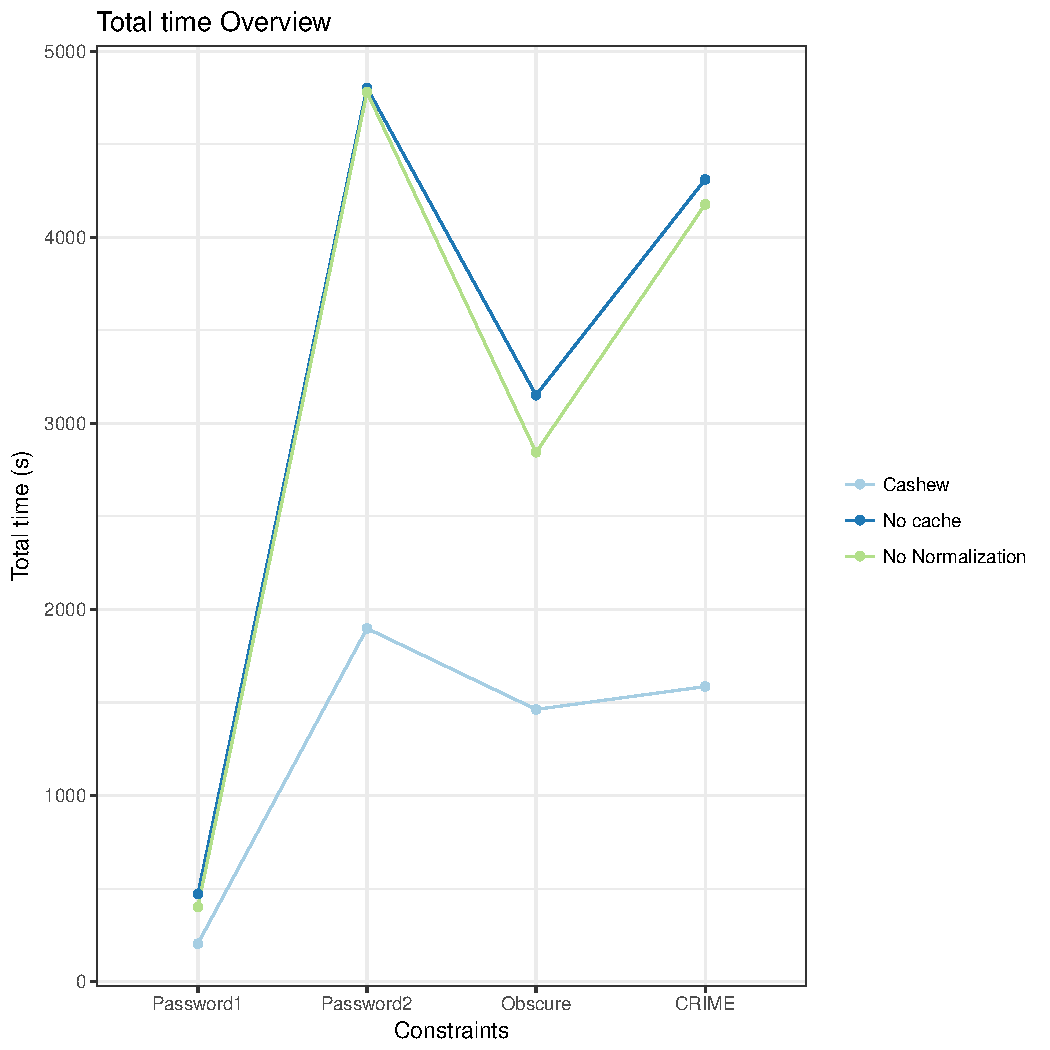
\includegraphics[width=\maxwidth]{figure/overview_sumTime-1} 

\end{knitrout}
\begin{knitrout}
\definecolor{shadecolor}{rgb}{0.969, 0.969, 0.969}\color{fgcolor}
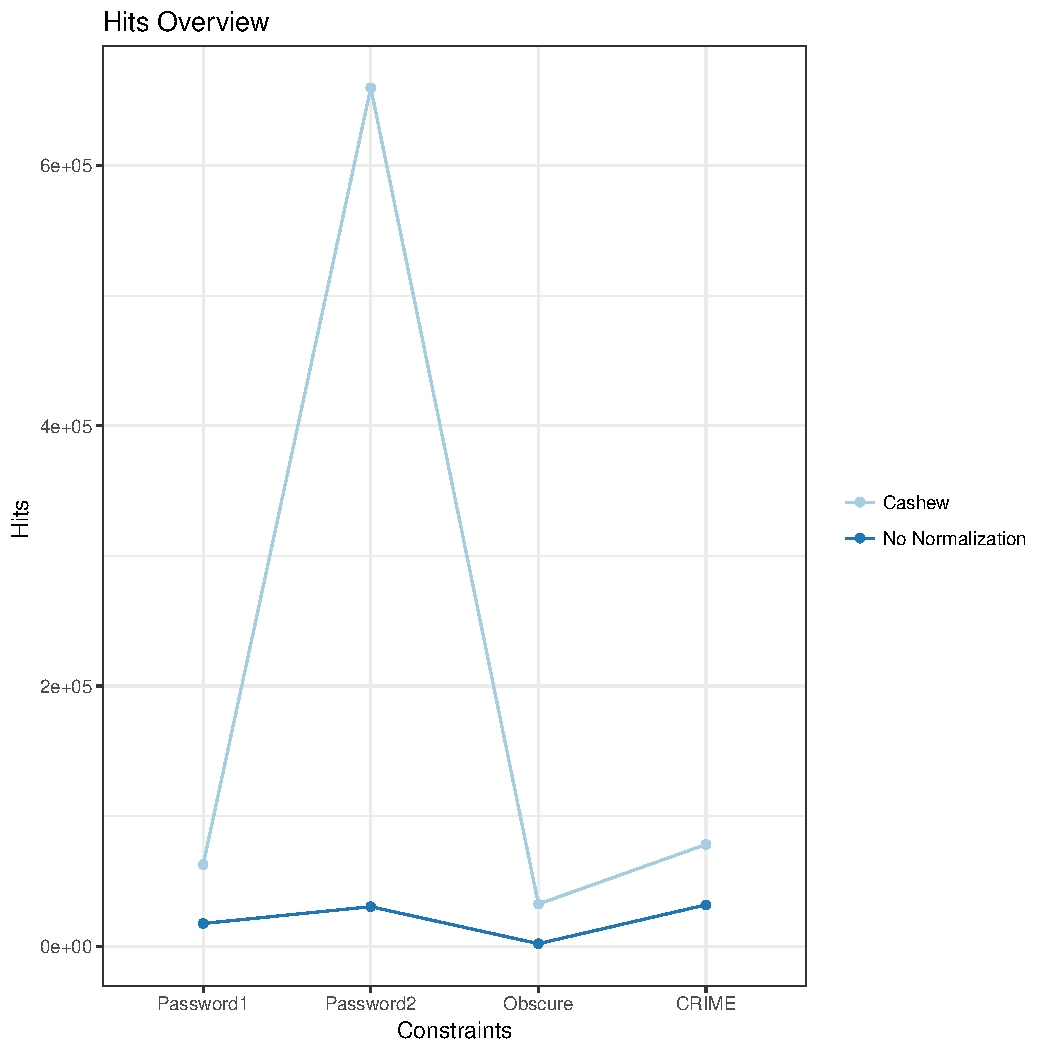
\includegraphics[width=\maxwidth]{figure/overview_hits-1} 

\end{knitrout}
\begin{knitrout}
\definecolor{shadecolor}{rgb}{0.969, 0.969, 0.969}\color{fgcolor}
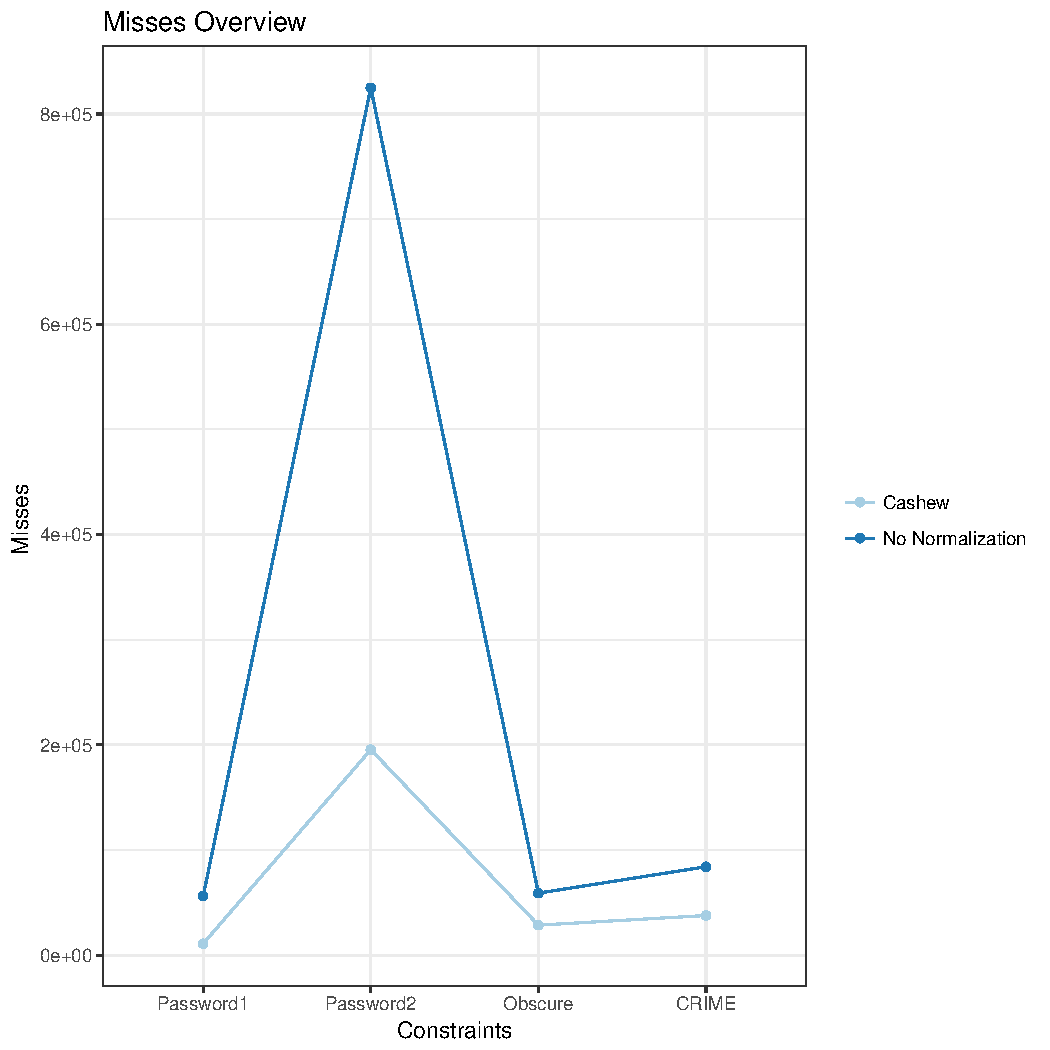
\includegraphics[width=\maxwidth]{figure/overview_misses-1} 

\end{knitrout}
\begin{knitrout}
\definecolor{shadecolor}{rgb}{0.969, 0.969, 0.969}\color{fgcolor}
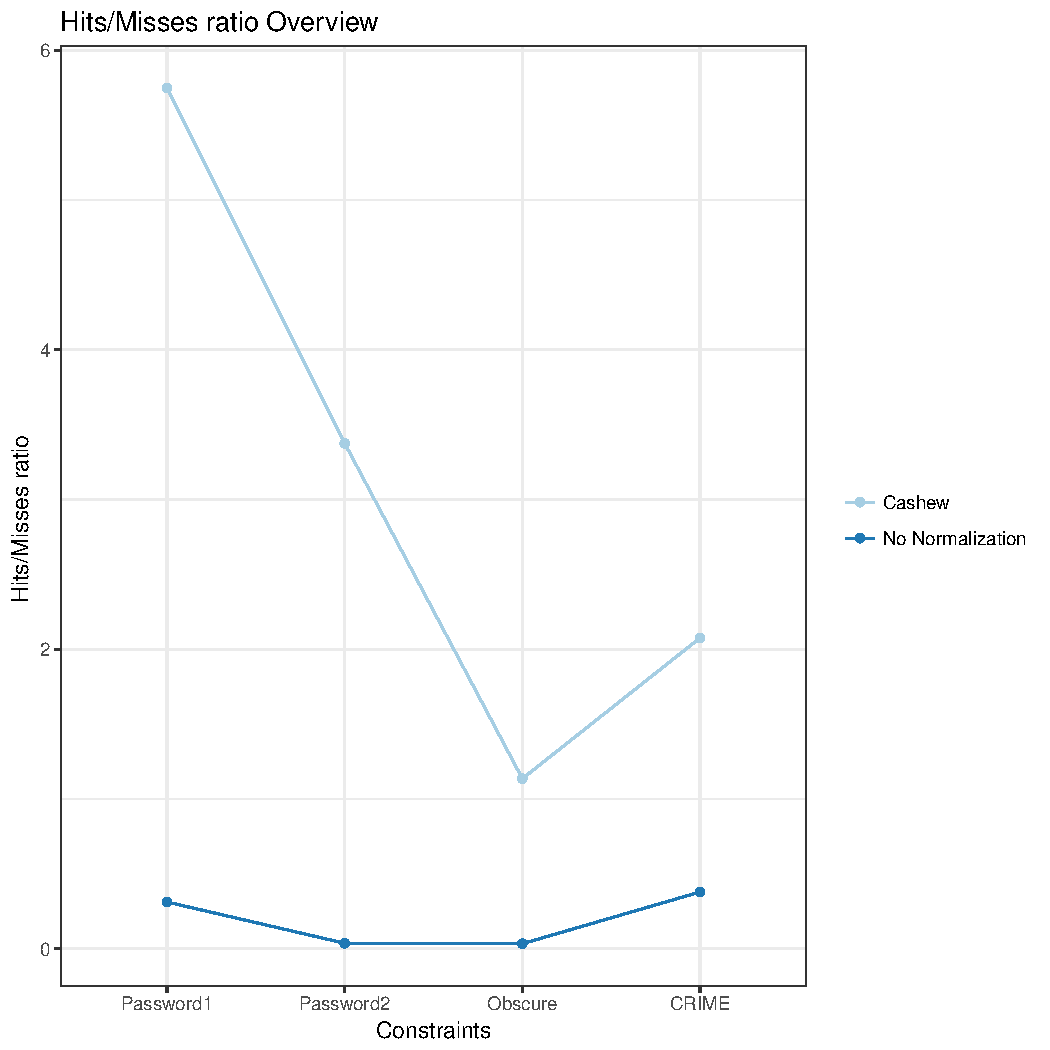
\includegraphics[width=\maxwidth]{figure/overview_hitsMissesRatio-1} 

\end{knitrout}



\subsection{Objects Overview}
\subsubsection{Overview for Password1}
\begin{knitrout}
\definecolor{shadecolor}{rgb}{0.969, 0.969, 0.969}\color{fgcolor}
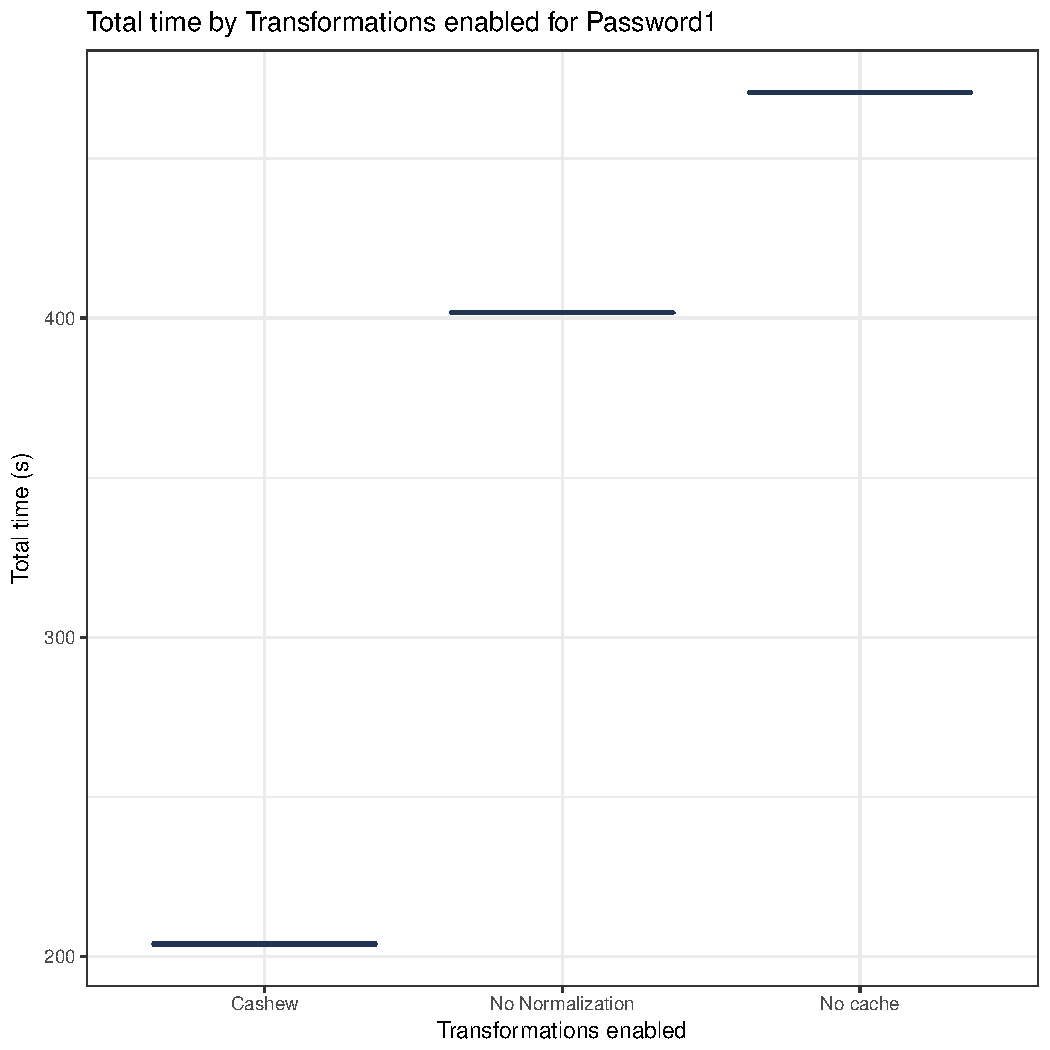
\includegraphics[width=\maxwidth]{figure/password-1} 

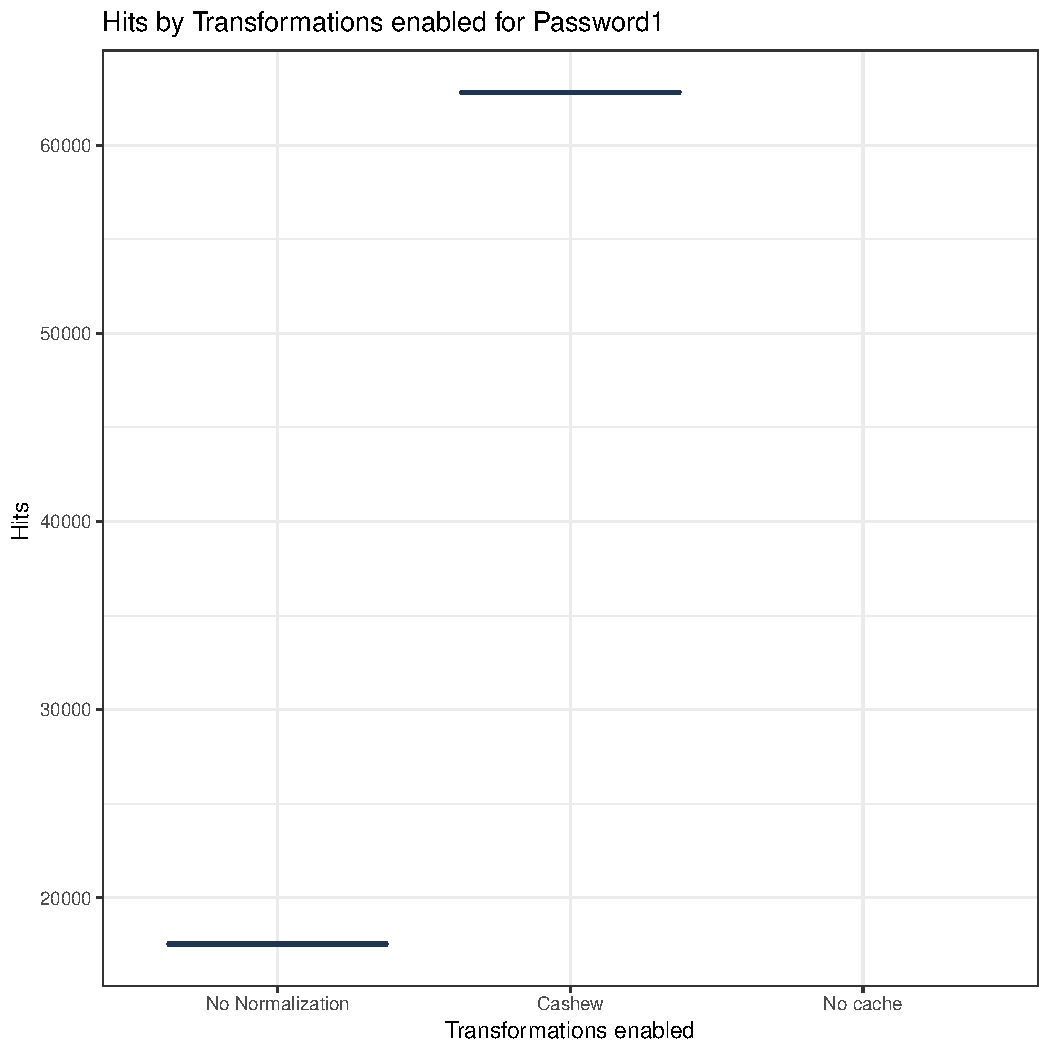
\includegraphics[width=\maxwidth]{figure/password-2} 

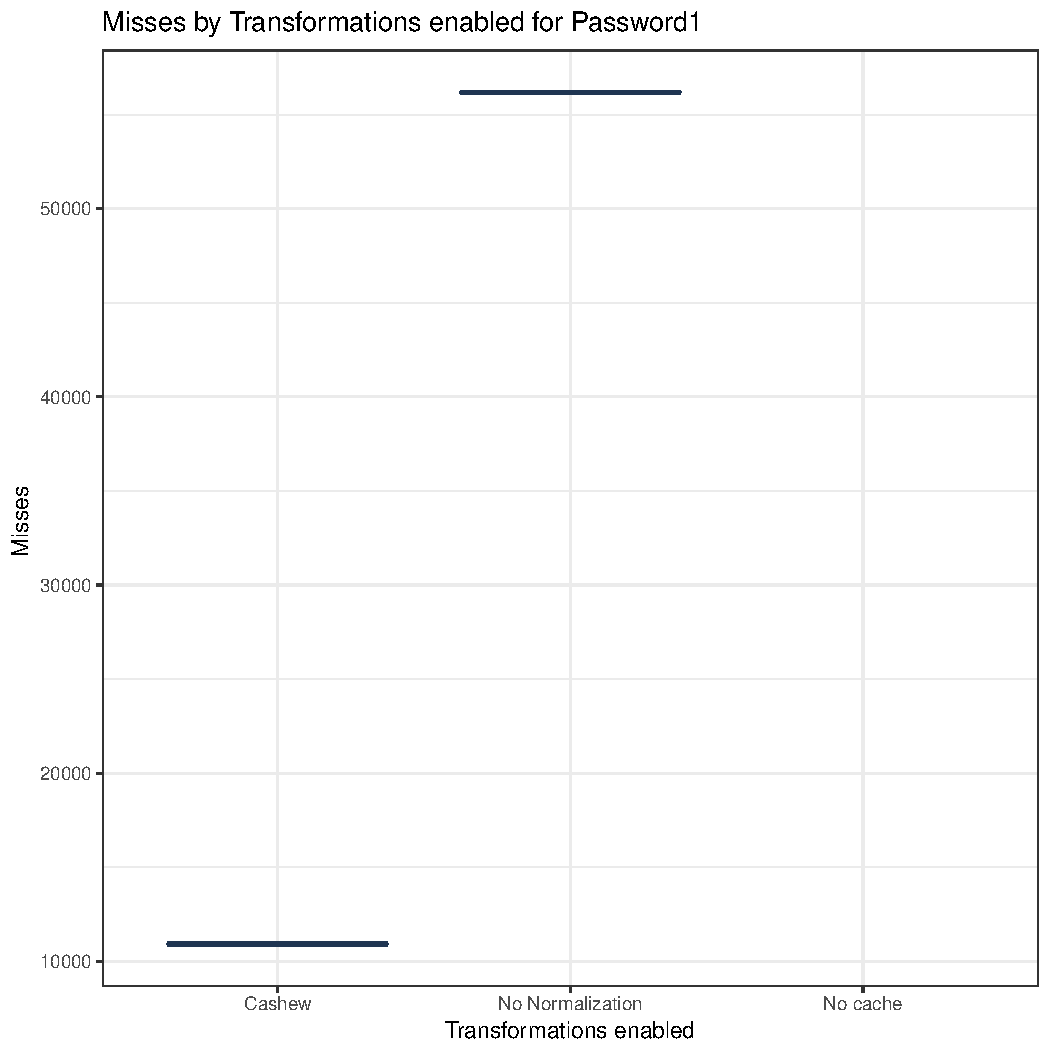
\includegraphics[width=\maxwidth]{figure/password-3} 

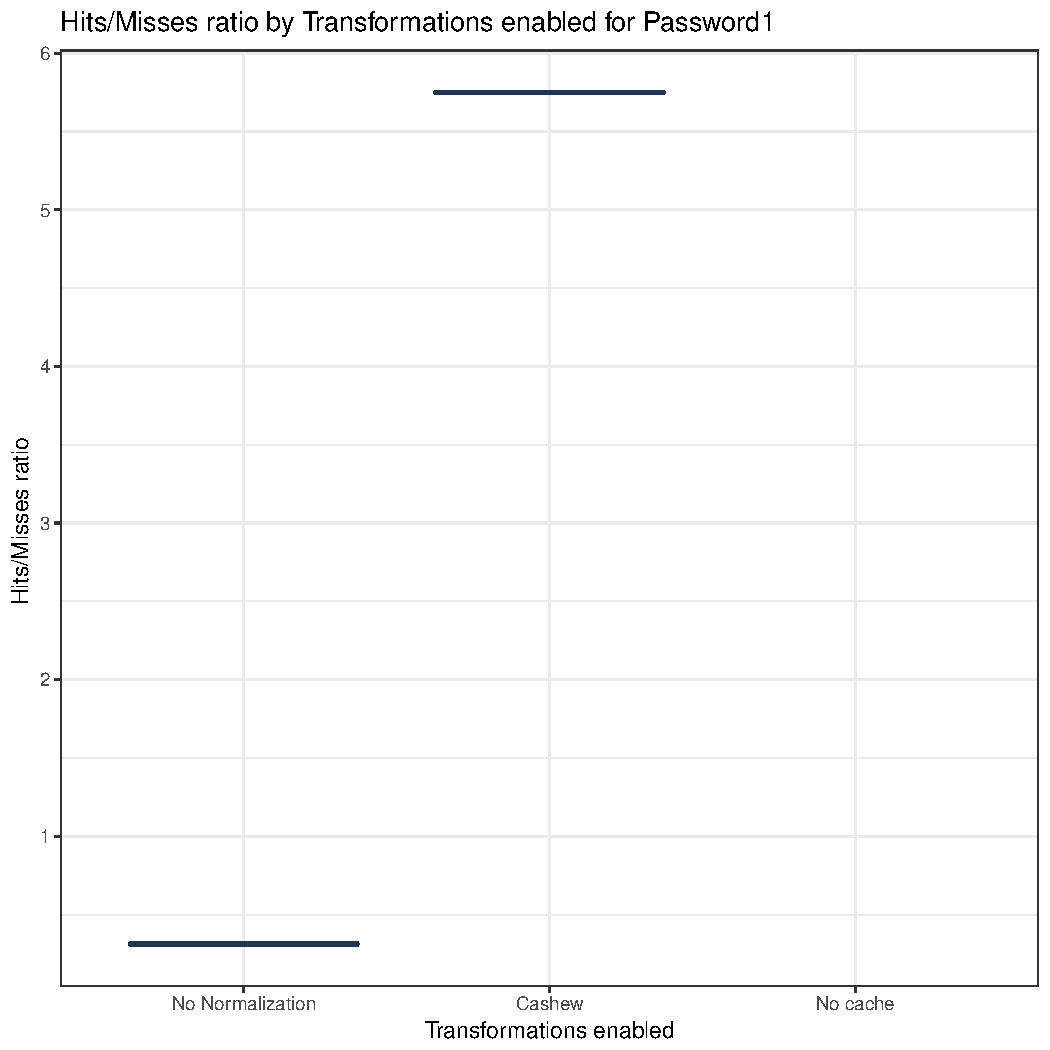
\includegraphics[width=\maxwidth]{figure/password-4} 

\end{knitrout}
\subsubsection{Overview for Password2}
\begin{knitrout}
\definecolor{shadecolor}{rgb}{0.969, 0.969, 0.969}\color{fgcolor}
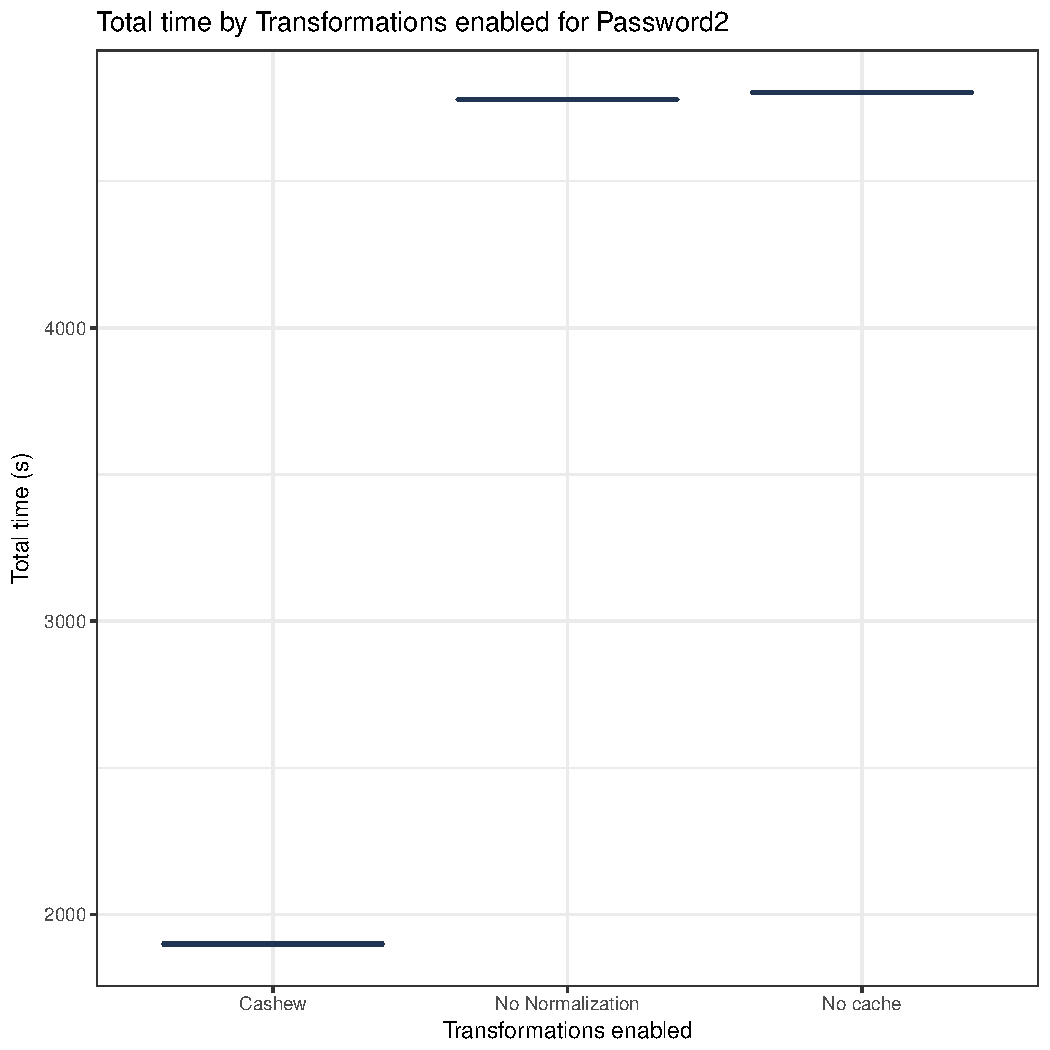
\includegraphics[width=\maxwidth]{figure/password2-1} 

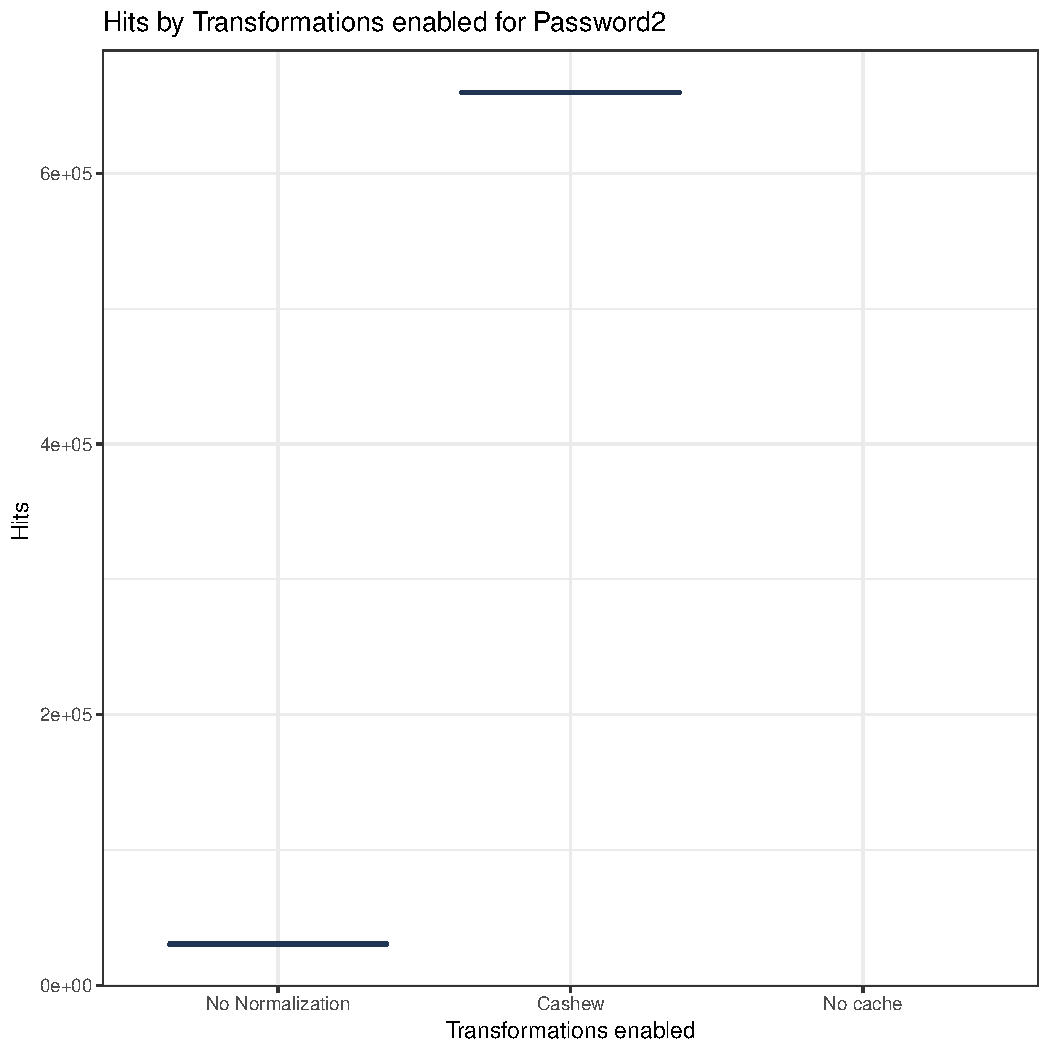
\includegraphics[width=\maxwidth]{figure/password2-2} 

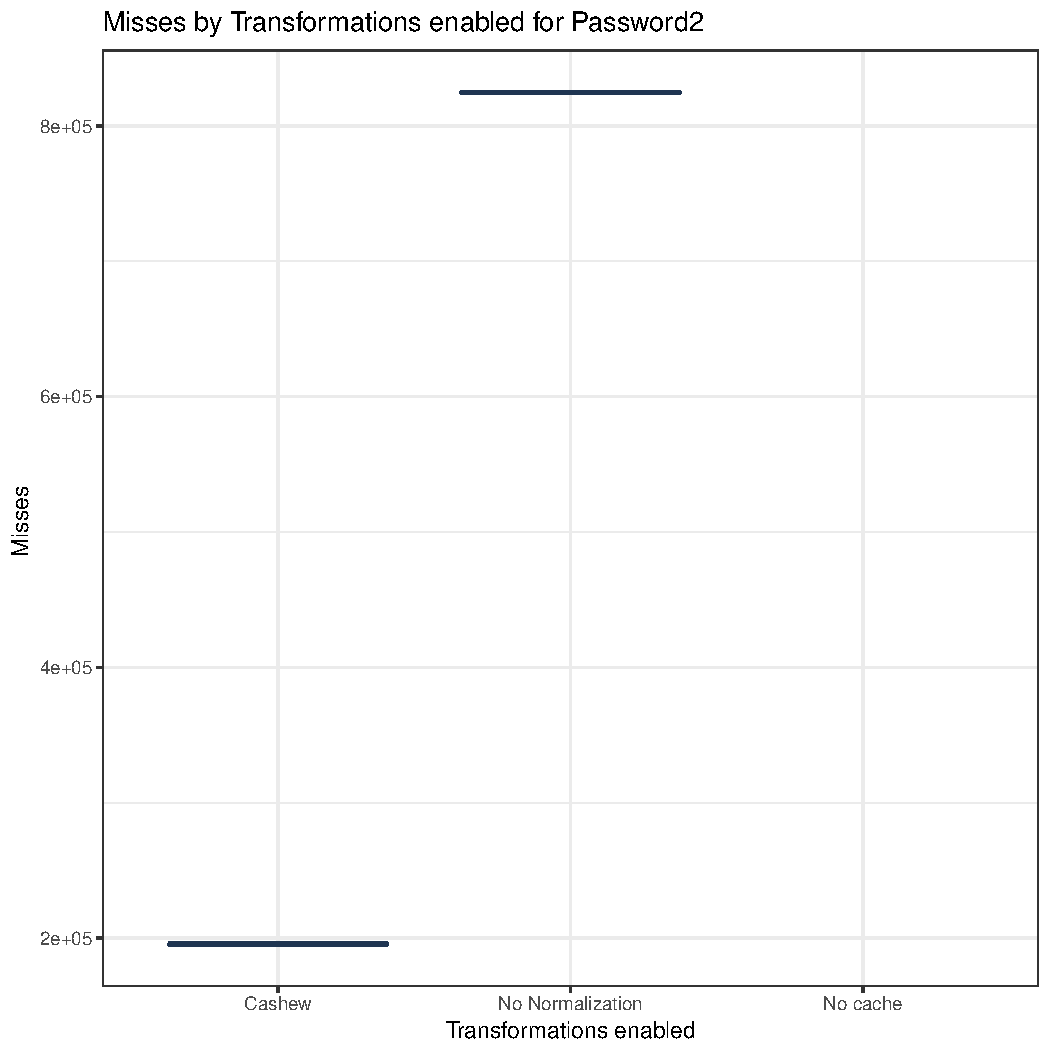
\includegraphics[width=\maxwidth]{figure/password2-3} 

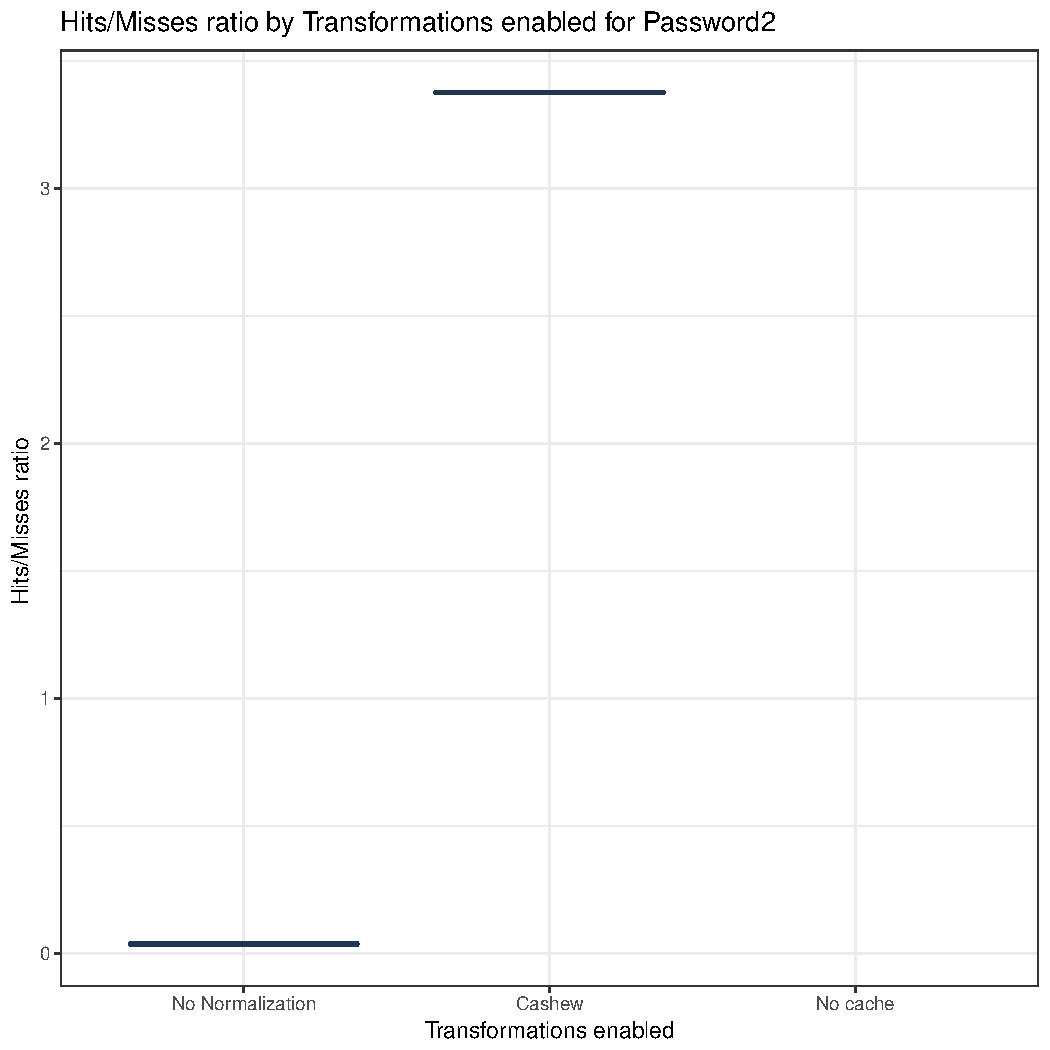
\includegraphics[width=\maxwidth]{figure/password2-4} 

\end{knitrout}
\subsubsection{Overview for Obscure}
\begin{knitrout}
\definecolor{shadecolor}{rgb}{0.969, 0.969, 0.969}\color{fgcolor}
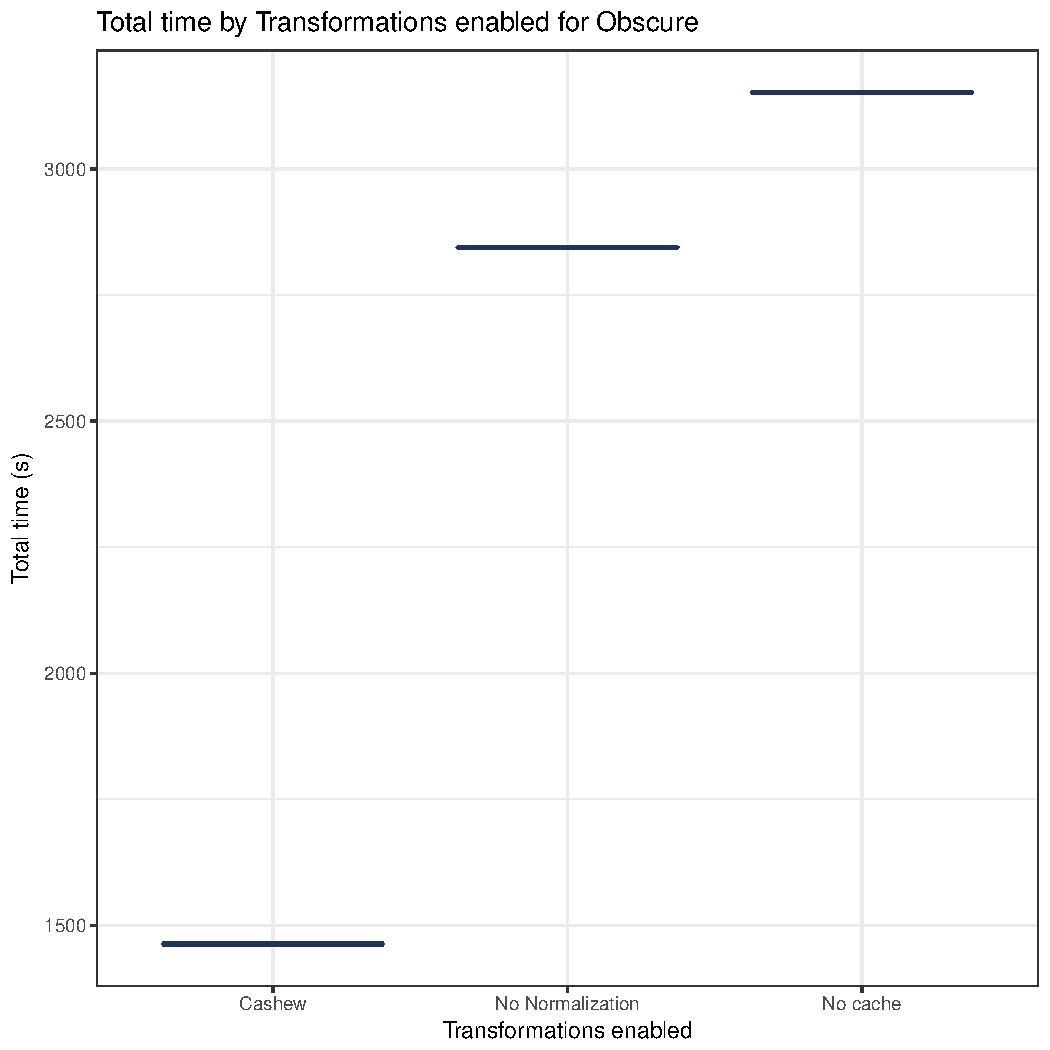
\includegraphics[width=\maxwidth]{figure/obscure-1} 

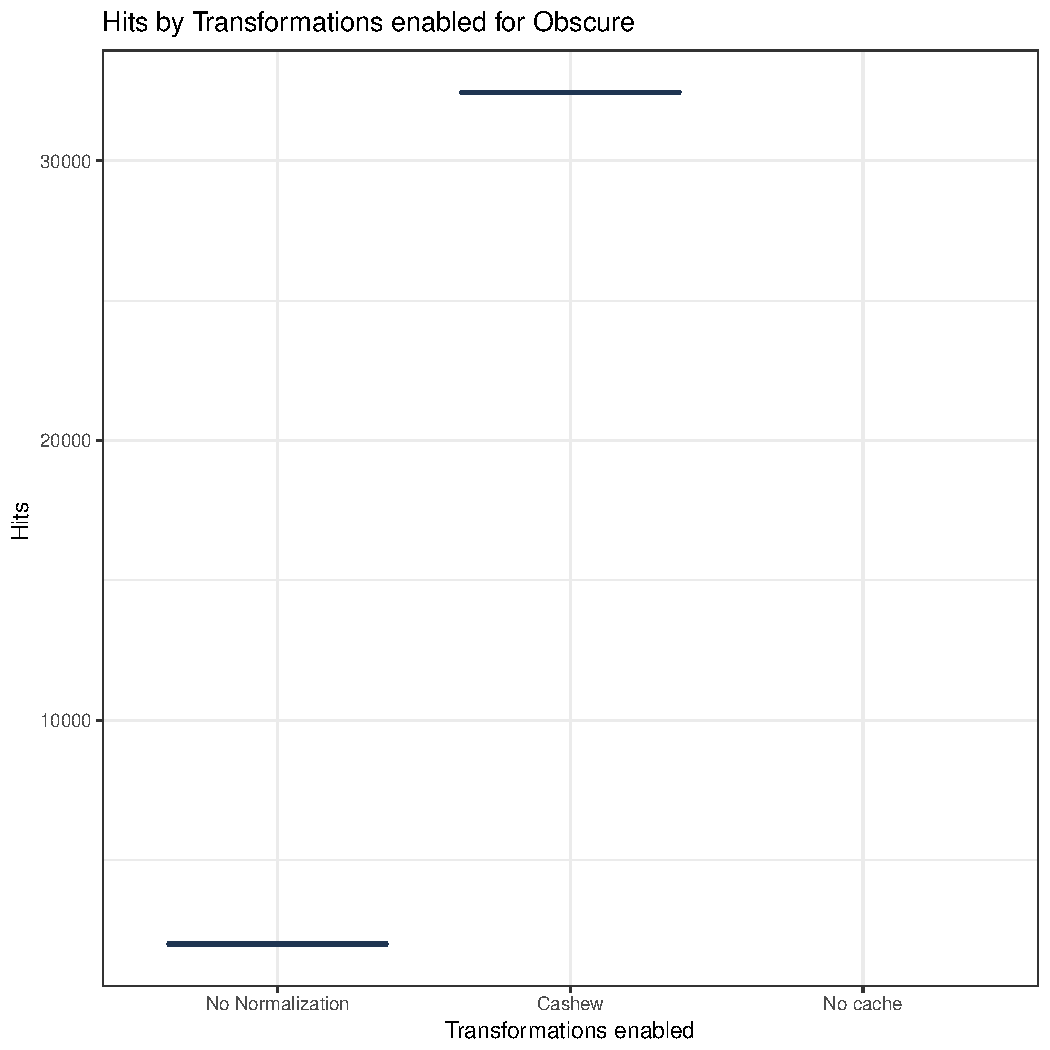
\includegraphics[width=\maxwidth]{figure/obscure-2} 

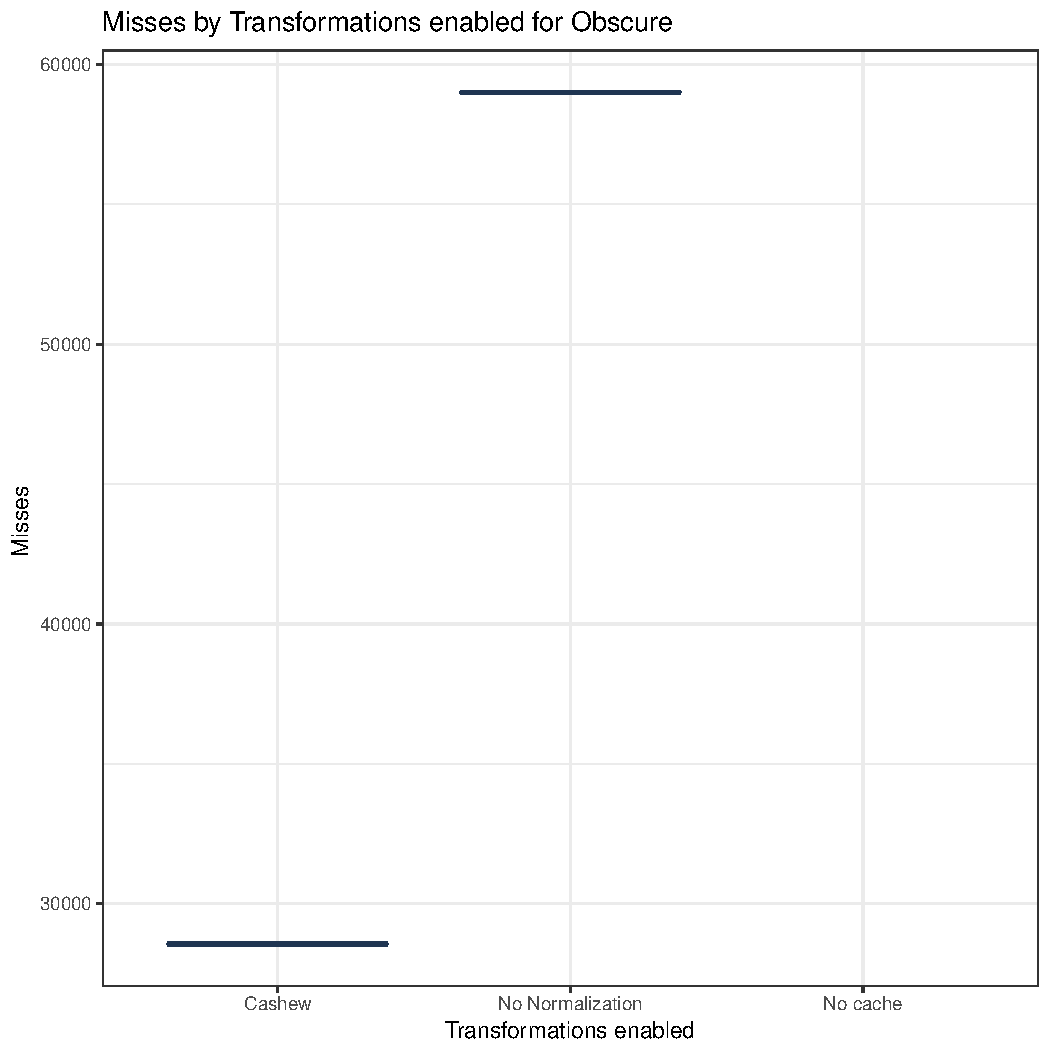
\includegraphics[width=\maxwidth]{figure/obscure-3} 

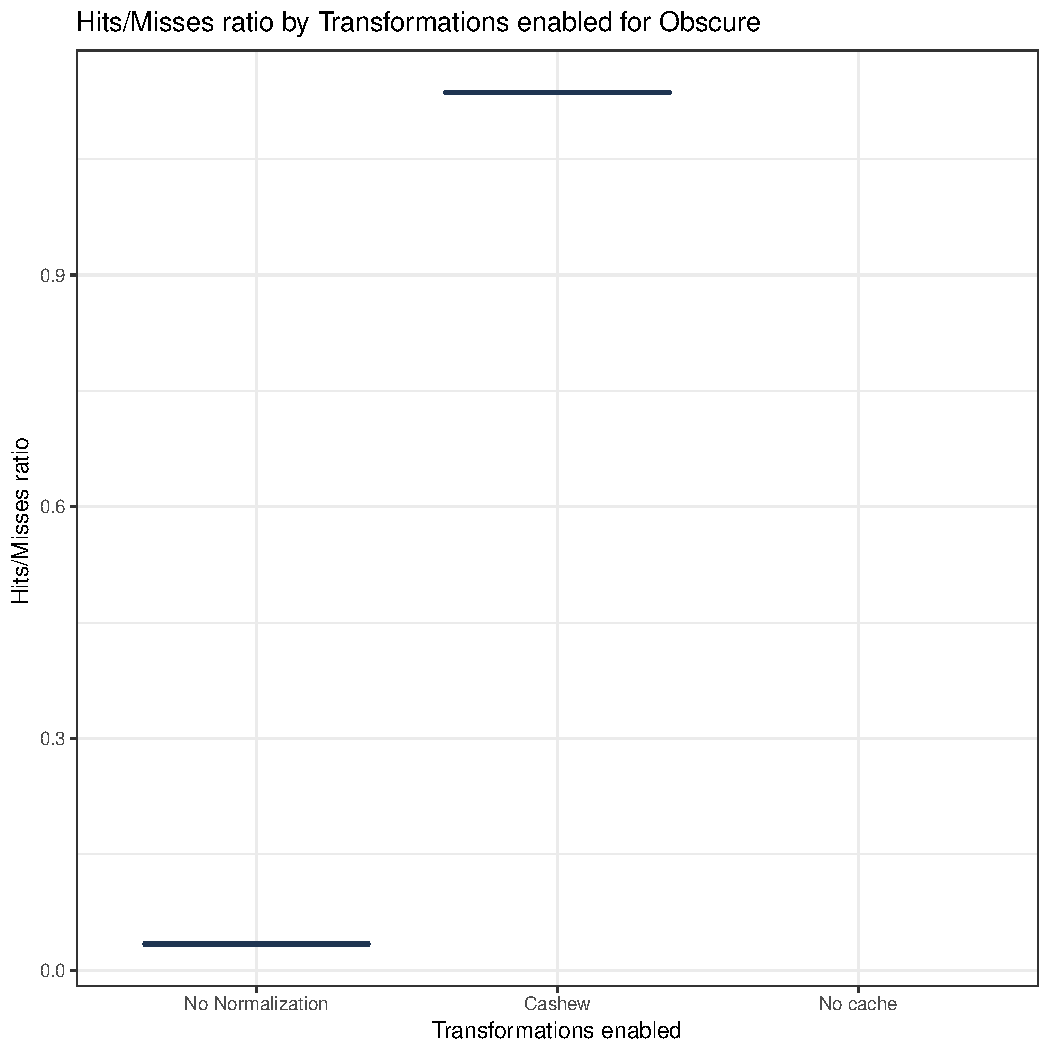
\includegraphics[width=\maxwidth]{figure/obscure-4} 

\end{knitrout}
\subsubsection{Overview for CRIME}
\begin{knitrout}
\definecolor{shadecolor}{rgb}{0.969, 0.969, 0.969}\color{fgcolor}
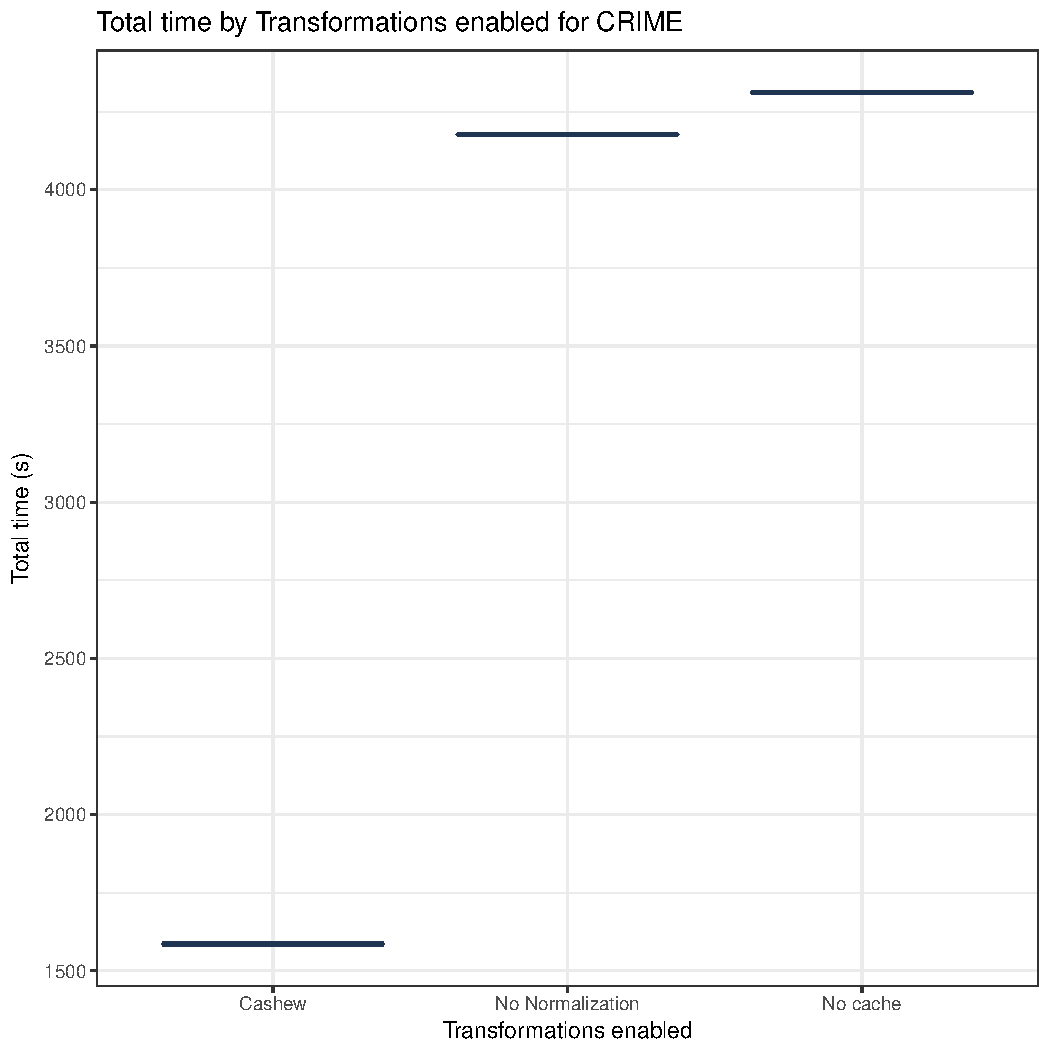
\includegraphics[width=\maxwidth]{figure/crime-1} 

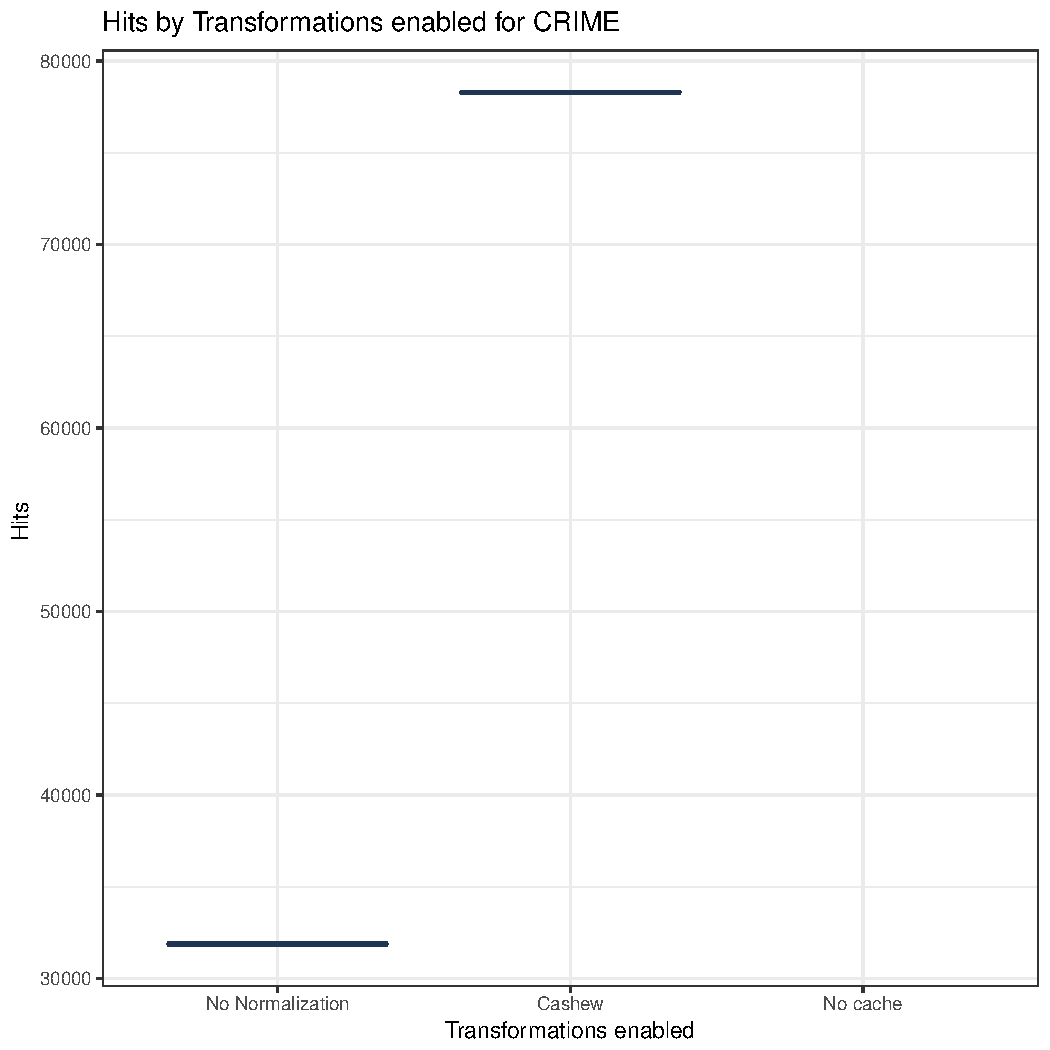
\includegraphics[width=\maxwidth]{figure/crime-2} 

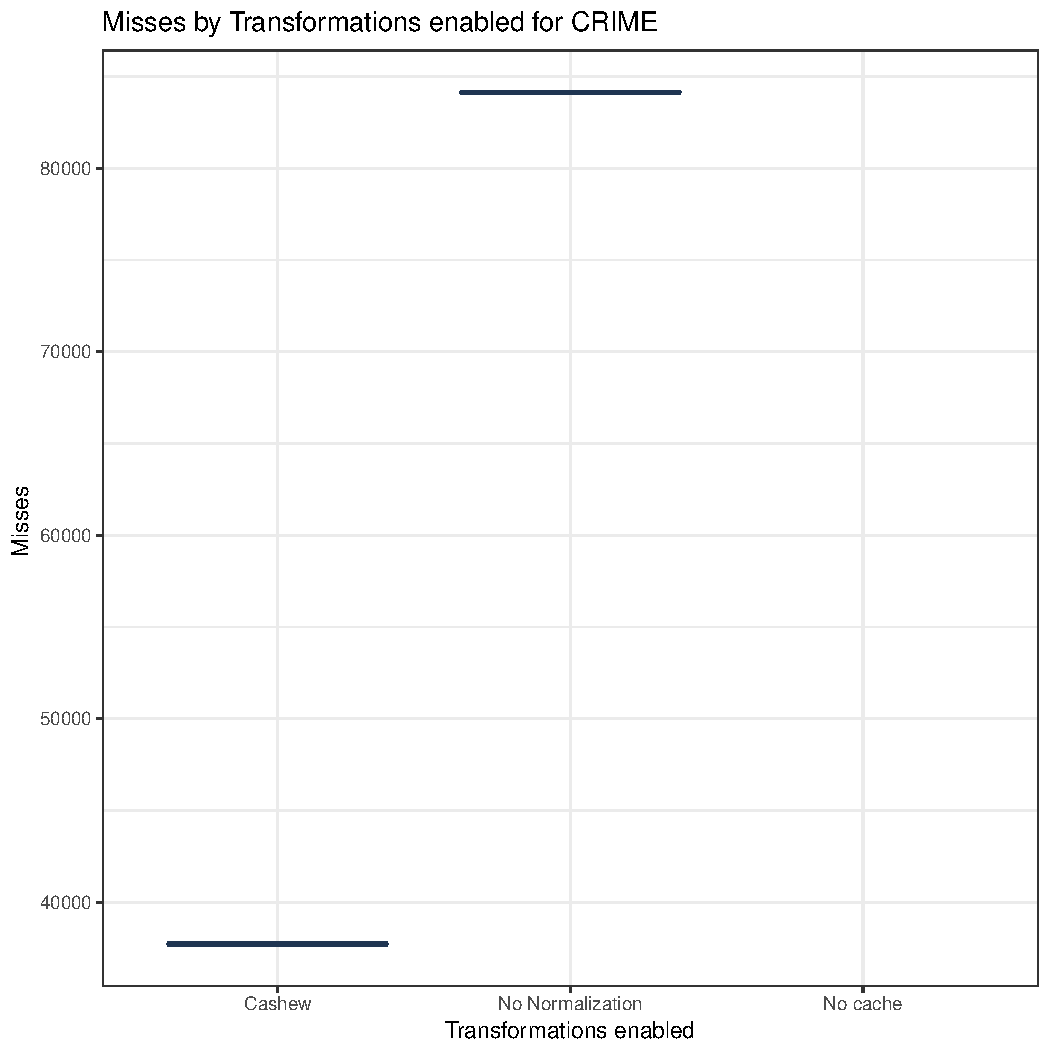
\includegraphics[width=\maxwidth]{figure/crime-3} 

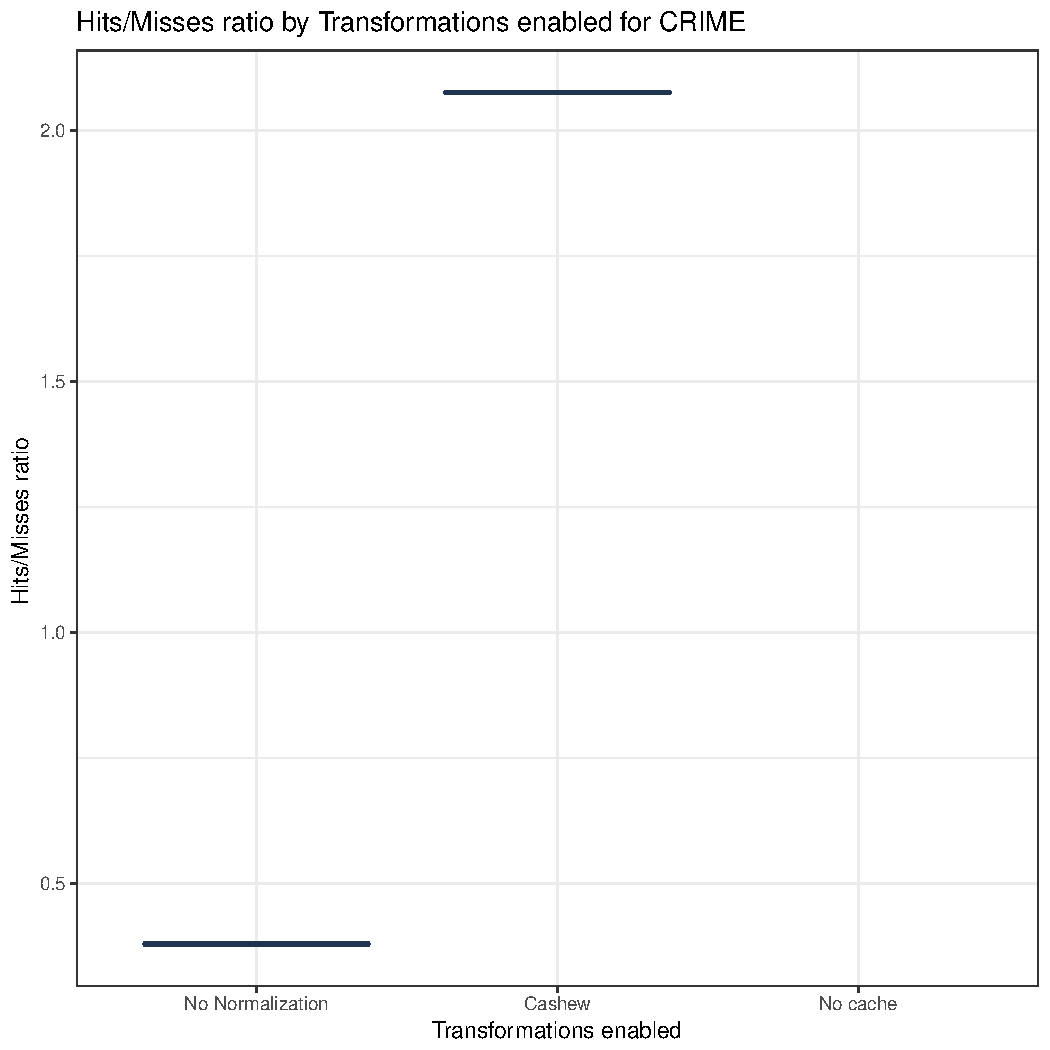
\includegraphics[width=\maxwidth]{figure/crime-4} 

\end{knitrout}

\section{Research Hypotheses}

\subsection{RH1: Total time for Cashew is equals than Total time for No Cache}


 
\begin{knitrout}
\definecolor{shadecolor}{rgb}{0.969, 0.969, 0.969}\color{fgcolor}
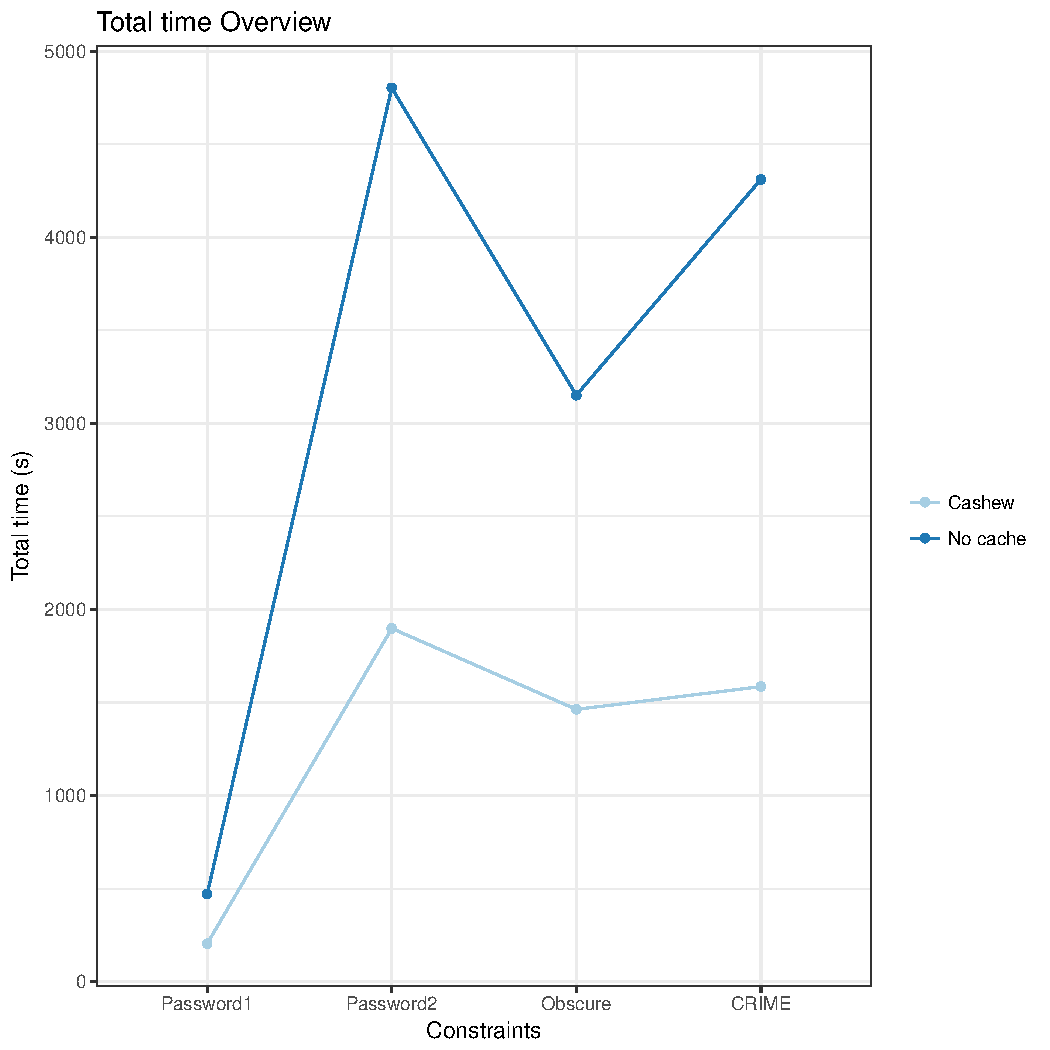
\includegraphics[width=\maxwidth]{figure/overview_RH1-1} 

\end{knitrout}
 	

\subsubsection{RH1.1: Object Password1}

 \textbf{Total time for Cashew}
\begin{knitrout}
\definecolor{shadecolor}{rgb}{0.969, 0.969, 0.969}\color{fgcolor}\begin{kframe}
\begin{verbatim}
## [1] "Sample size:  1"
##    Min. 1st Qu.  Median    Mean 3rd Qu.    Max. 
##   203.9   203.9   203.9   203.9   203.9   203.9
\end{verbatim}


{\ttfamily\noindent\bfseries\color{errorcolor}{\#\# Error in shapiro.test(subset(json\_data, treatment == "{}cashew"{} \& object == : sample size must be between 3 and 5000}}\end{kframe}
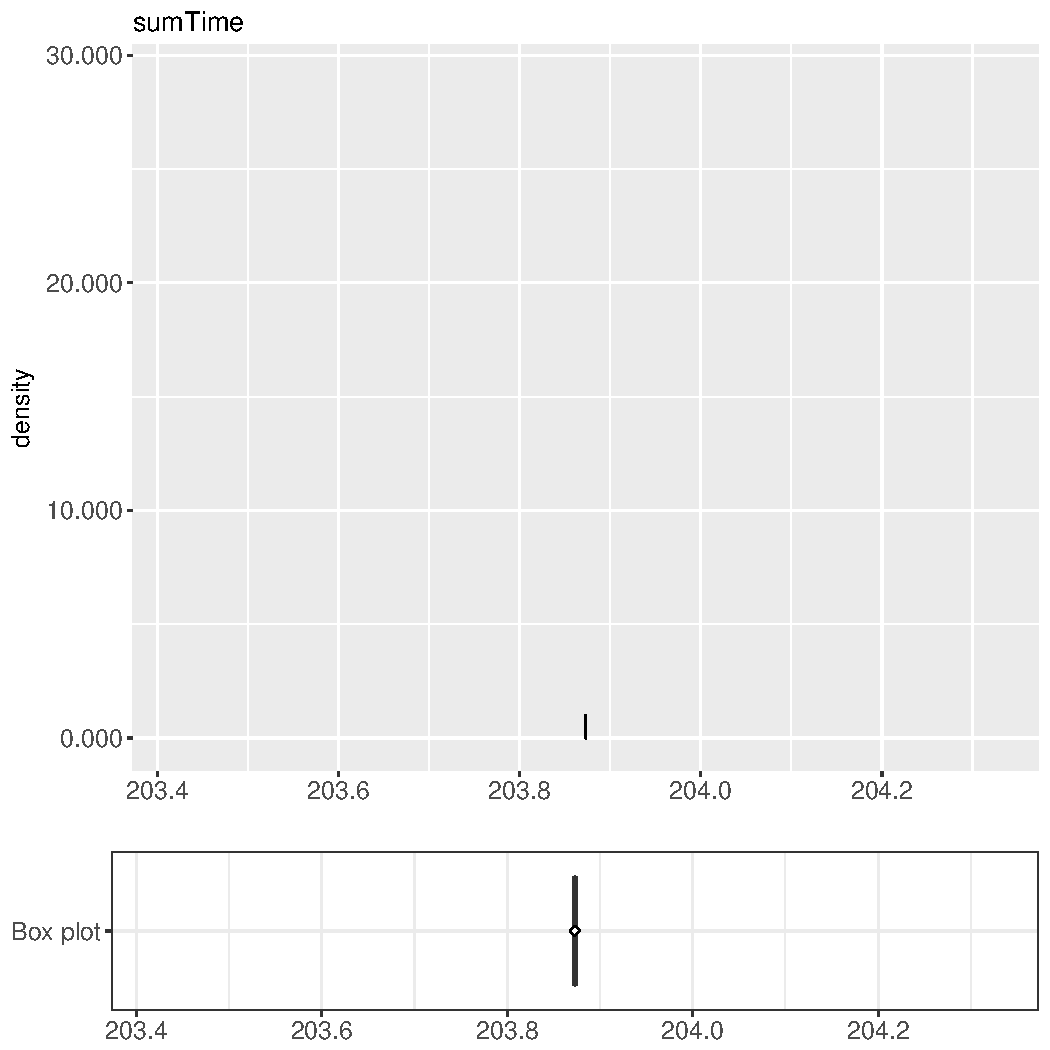
\includegraphics[width=\maxwidth]{figure/RH1_cashew_password-1} 

\end{knitrout}
 \textbf{Total time for No cache}
\begin{knitrout}
\definecolor{shadecolor}{rgb}{0.969, 0.969, 0.969}\color{fgcolor}\begin{kframe}
\begin{verbatim}
## [1] "Sample size:  1"
##    Min. 1st Qu.  Median    Mean 3rd Qu.    Max. 
##   470.7   470.7   470.7   470.7   470.7   470.7
\end{verbatim}


{\ttfamily\noindent\bfseries\color{errorcolor}{\#\# Error in shapiro.test(subset(json\_data, treatment == "{}nocache"{} \& object == : sample size must be between 3 and 5000}}\end{kframe}
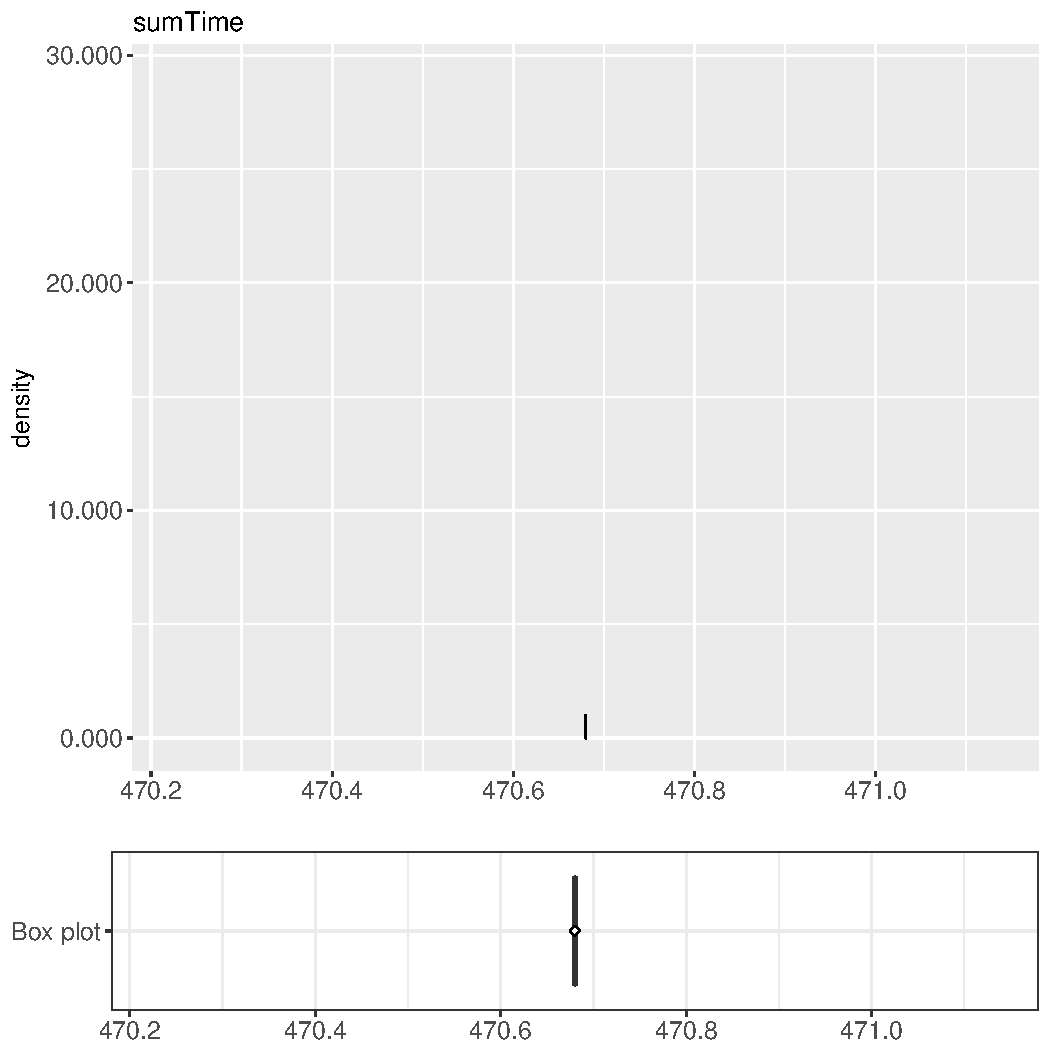
\includegraphics[width=\maxwidth]{figure/RH1_nocache_password-1} 

\end{knitrout}
  
 \textbf{Comparison}
  
\begin{knitrout}
\definecolor{shadecolor}{rgb}{0.969, 0.969, 0.969}\color{fgcolor}
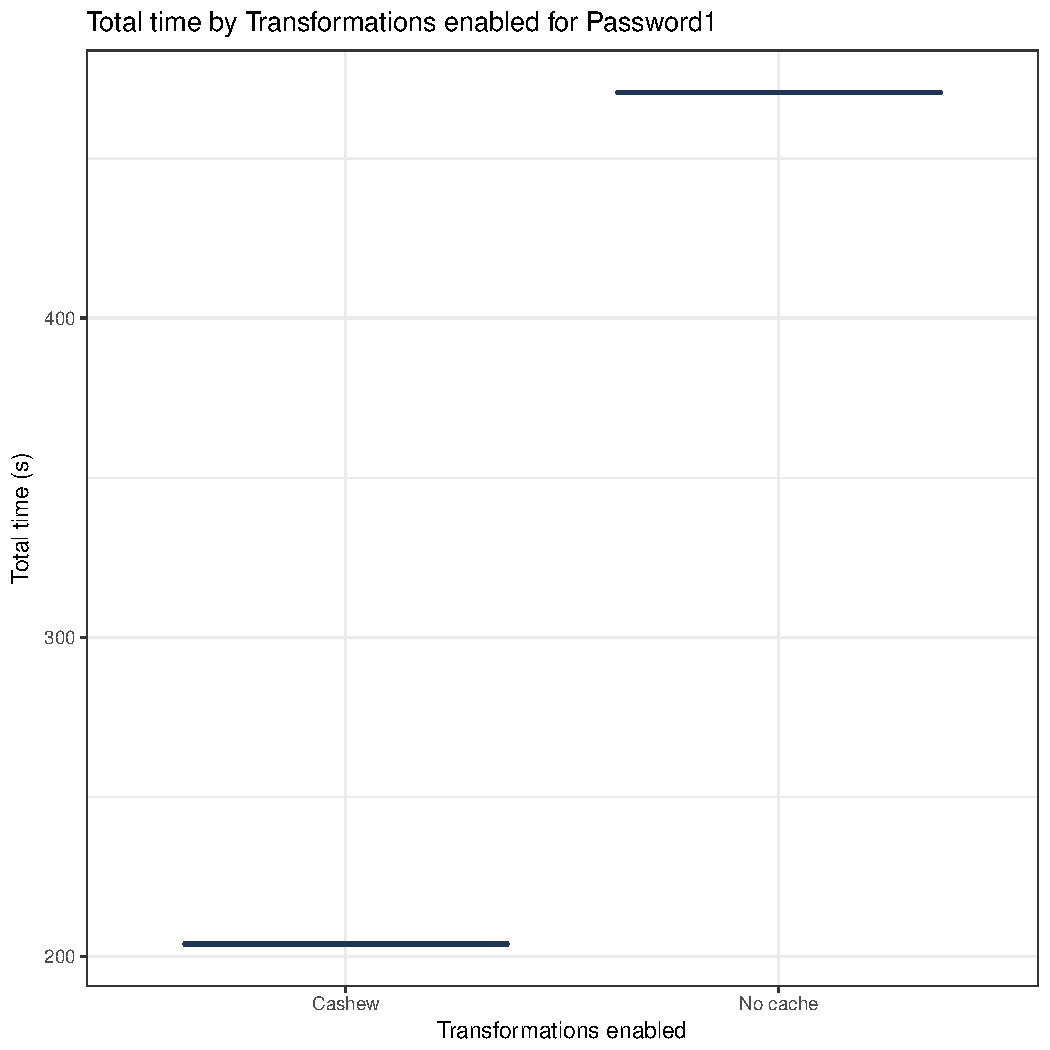
\includegraphics[width=\maxwidth]{figure/RH1_password-1} 
\begin{kframe}

{\ttfamily\noindent\bfseries\color{errorcolor}{\#\# Error in eval(expr, envir, enclos): object 'shap\_cashew\_password' not found}}\begin{verbatim}
## [1] ""
## [1] "Means comparison"
## [1] "Mean Total time for Cashew:  203.873"
## [1] "Mean Total time for No cache:  470.68"
## [1] "Absolute difference:  266.807"
## Total time for No cache is  130.869217601154 % greater than 
## Total time for Cashew
\end{verbatim}
\end{kframe}
\end{knitrout}


\subsubsection{RH1.2: Object Password2}

 \textbf{Total time for Cashew}
\begin{knitrout}
\definecolor{shadecolor}{rgb}{0.969, 0.969, 0.969}\color{fgcolor}\begin{kframe}
\begin{verbatim}
## [1] "Sample size:  1"
##    Min. 1st Qu.  Median    Mean 3rd Qu.    Max. 
##    1898    1898    1898    1898    1898    1898
\end{verbatim}


{\ttfamily\noindent\bfseries\color{errorcolor}{\#\# Error in shapiro.test(subset(json\_data, treatment == "{}cashew"{} \& object == : sample size must be between 3 and 5000}}\end{kframe}
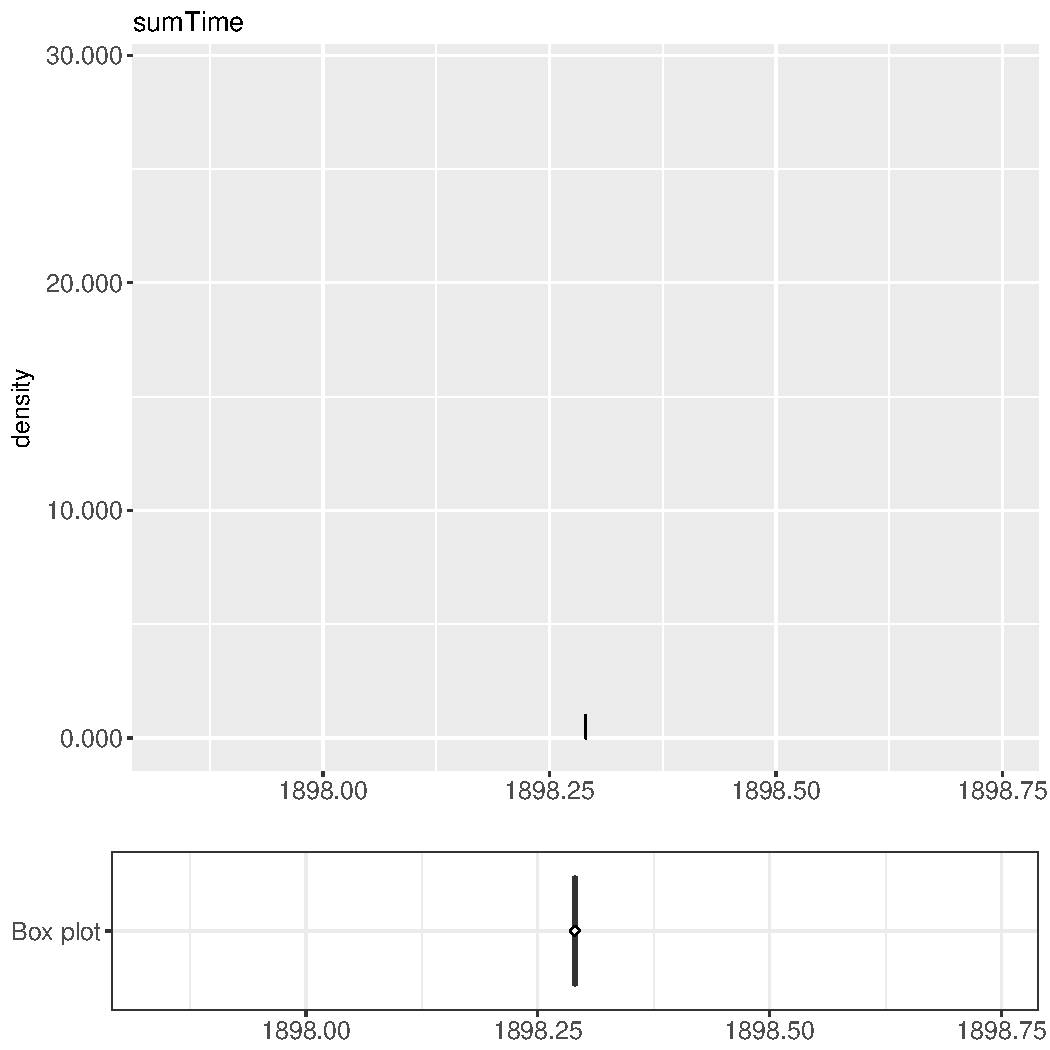
\includegraphics[width=\maxwidth]{figure/RH1_cashew_password2-1} 

\end{knitrout}
 \textbf{Total time for No cache}
\begin{knitrout}
\definecolor{shadecolor}{rgb}{0.969, 0.969, 0.969}\color{fgcolor}\begin{kframe}
\begin{verbatim}
## [1] "Sample size:  1"
##    Min. 1st Qu.  Median    Mean 3rd Qu.    Max. 
##    4803    4803    4803    4803    4803    4803
\end{verbatim}


{\ttfamily\noindent\bfseries\color{errorcolor}{\#\# Error in shapiro.test(subset(json\_data, treatment == "{}nocache"{} \& object == : sample size must be between 3 and 5000}}\end{kframe}
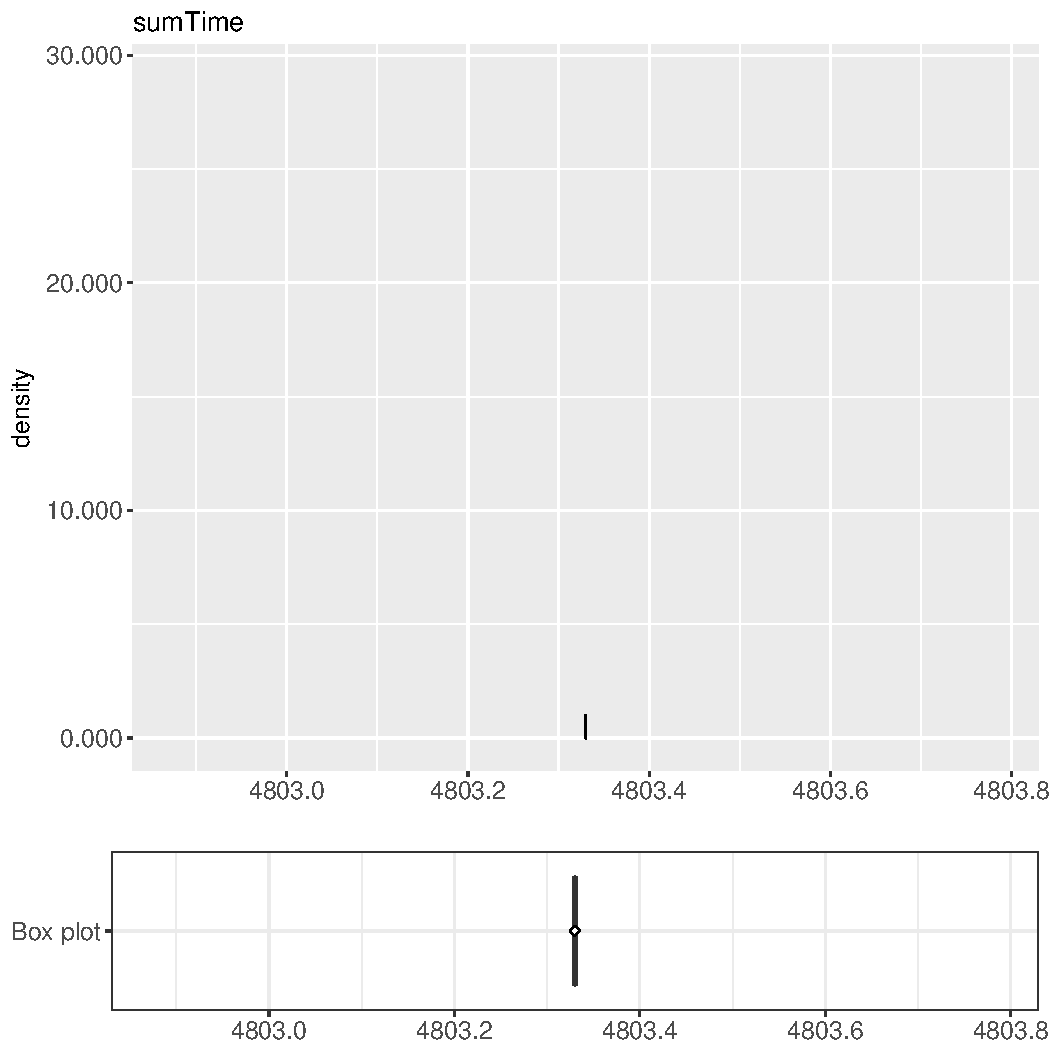
\includegraphics[width=\maxwidth]{figure/RH1_nocache_password2-1} 

\end{knitrout}
  
 \textbf{Comparison}
  
\begin{knitrout}
\definecolor{shadecolor}{rgb}{0.969, 0.969, 0.969}\color{fgcolor}
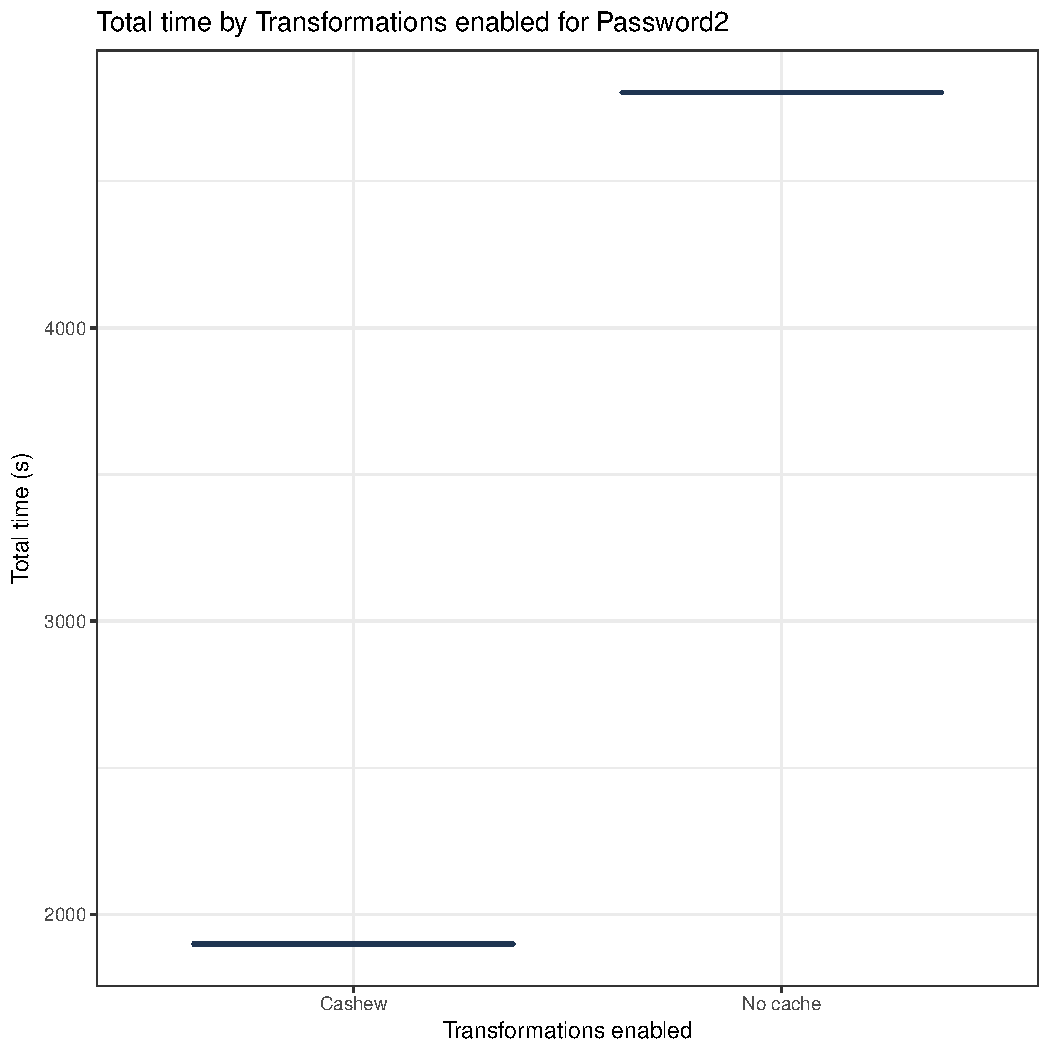
\includegraphics[width=\maxwidth]{figure/RH1_password2-1} 
\begin{kframe}

{\ttfamily\noindent\bfseries\color{errorcolor}{\#\# Error in eval(expr, envir, enclos): object 'shap\_cashew\_password2' not found}}\begin{verbatim}
## [1] ""
## [1] "Means comparison"
## [1] "Mean Total time for Cashew:  1898.29"
## [1] "Mean Total time for No cache:  4803.33"
## [1] "Absolute difference:  2905.04"
## Total time for No cache is  153.034573221162 % greater than 
## Total time for Cashew
\end{verbatim}
\end{kframe}
\end{knitrout}


\subsubsection{RH1.3: Object Obscure}

 \textbf{Total time for Cashew}
\begin{knitrout}
\definecolor{shadecolor}{rgb}{0.969, 0.969, 0.969}\color{fgcolor}\begin{kframe}
\begin{verbatim}
## [1] "Sample size:  1"
##    Min. 1st Qu.  Median    Mean 3rd Qu.    Max. 
##    1463    1463    1463    1463    1463    1463
\end{verbatim}


{\ttfamily\noindent\bfseries\color{errorcolor}{\#\# Error in shapiro.test(subset(json\_data, treatment == "{}cashew"{} \& object == : sample size must be between 3 and 5000}}\end{kframe}
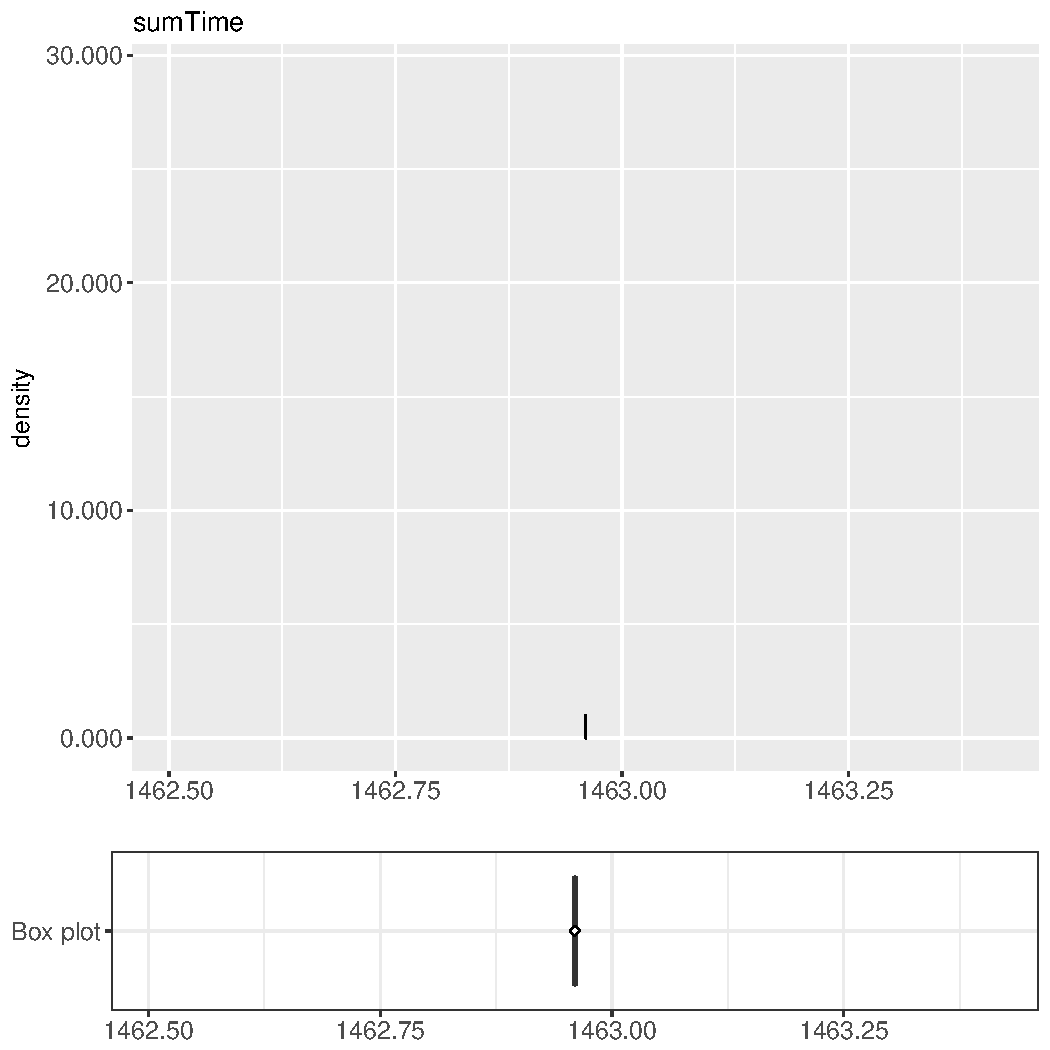
\includegraphics[width=\maxwidth]{figure/RH1_cashew_obscure-1} 

\end{knitrout}
 \textbf{Total time for No cache}
\begin{knitrout}
\definecolor{shadecolor}{rgb}{0.969, 0.969, 0.969}\color{fgcolor}\begin{kframe}
\begin{verbatim}
## [1] "Sample size:  1"
##    Min. 1st Qu.  Median    Mean 3rd Qu.    Max. 
##    3152    3152    3152    3152    3152    3152
\end{verbatim}


{\ttfamily\noindent\bfseries\color{errorcolor}{\#\# Error in shapiro.test(subset(json\_data, treatment == "{}nocache"{} \& object == : sample size must be between 3 and 5000}}\end{kframe}
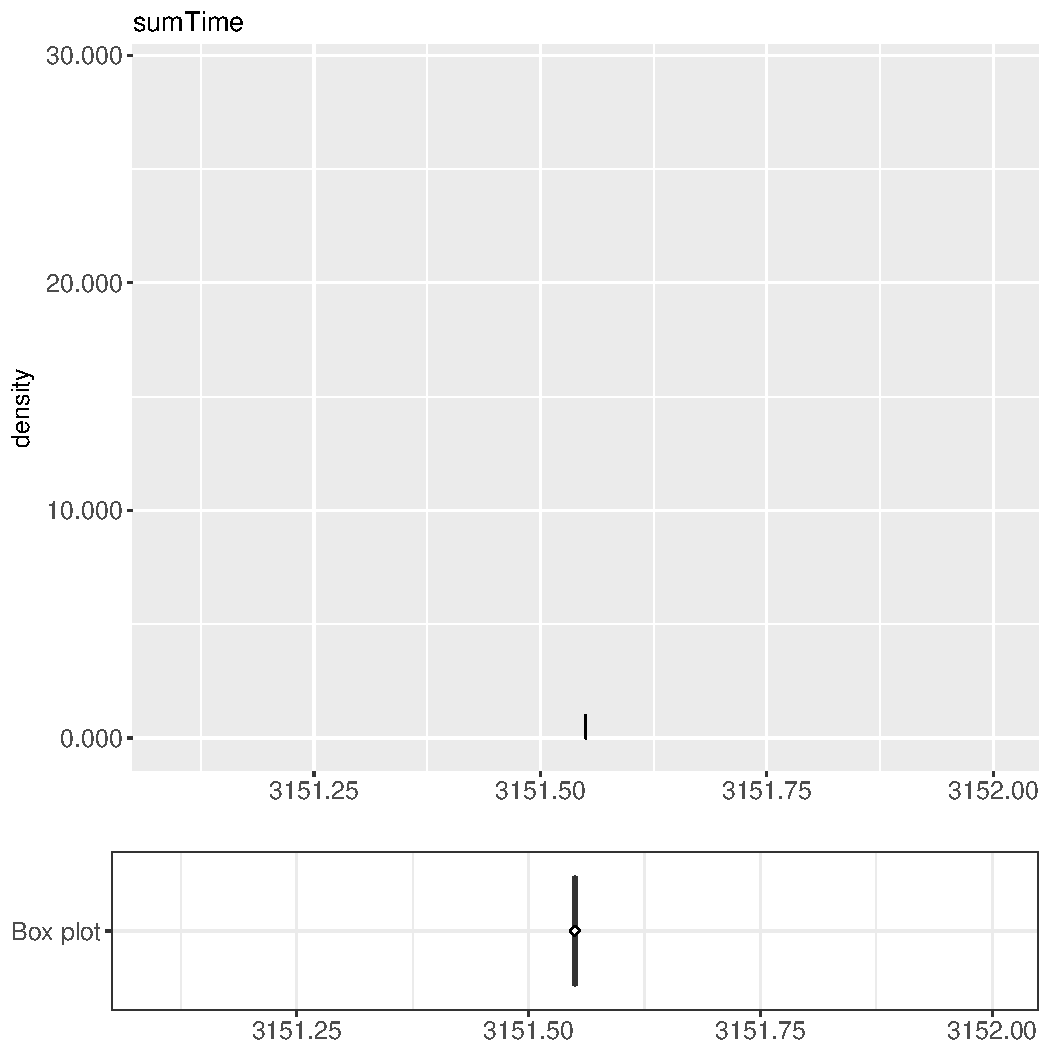
\includegraphics[width=\maxwidth]{figure/RH1_nocache_obscure-1} 

\end{knitrout}
  
 \textbf{Comparison}
  
\begin{knitrout}
\definecolor{shadecolor}{rgb}{0.969, 0.969, 0.969}\color{fgcolor}
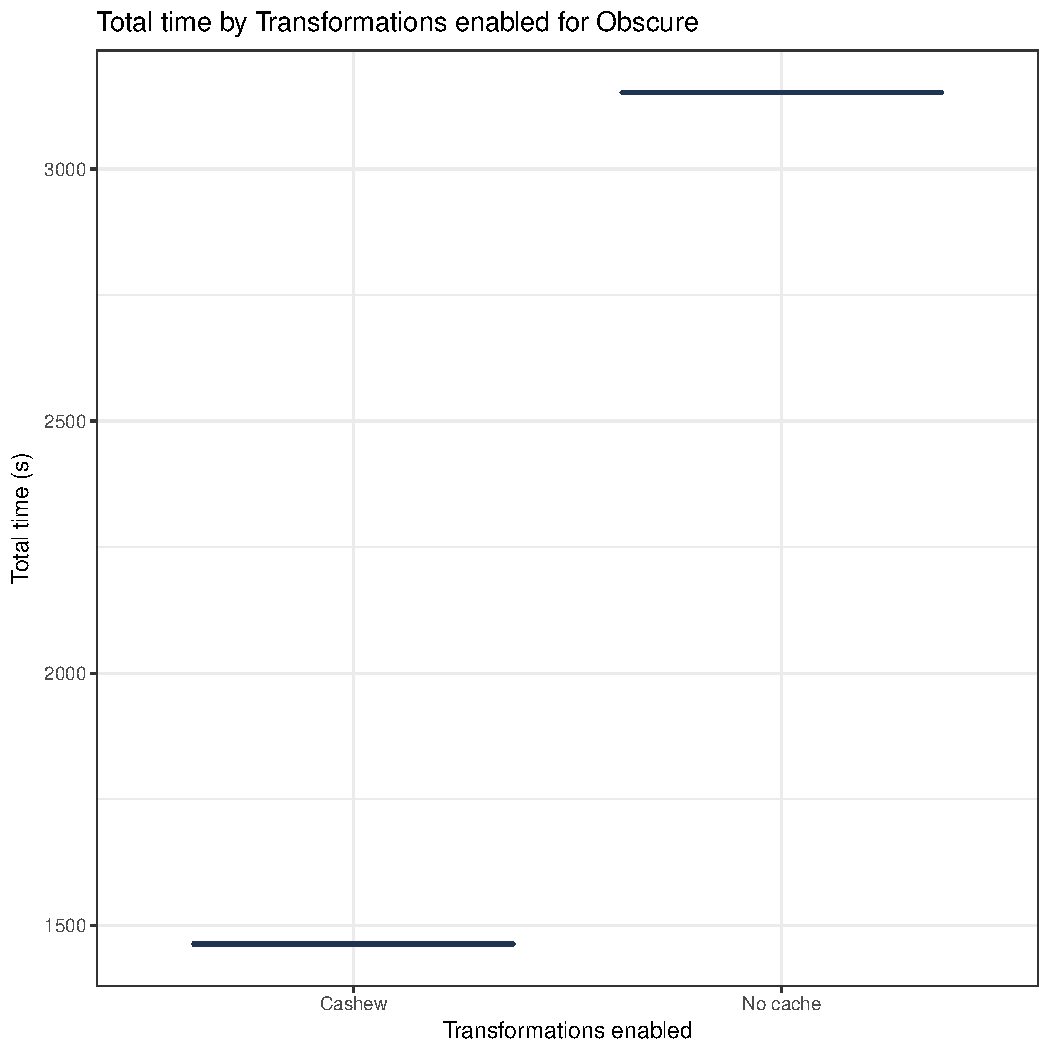
\includegraphics[width=\maxwidth]{figure/RH1_obscure-1} 
\begin{kframe}

{\ttfamily\noindent\bfseries\color{errorcolor}{\#\# Error in eval(expr, envir, enclos): object 'shap\_cashew\_obscure' not found}}\begin{verbatim}
## [1] ""
## [1] "Means comparison"
## [1] "Mean Total time for Cashew:  1462.96"
## [1] "Mean Total time for No cache:  3151.55"
## [1] "Absolute difference:  1688.59"
## Total time for No cache is  115.422841362717 % greater than 
## Total time for Cashew
\end{verbatim}
\end{kframe}
\end{knitrout}


\subsubsection{RH1.4: Object CRIME}

 \textbf{Total time for Cashew}
\begin{knitrout}
\definecolor{shadecolor}{rgb}{0.969, 0.969, 0.969}\color{fgcolor}\begin{kframe}
\begin{verbatim}
## [1] "Sample size:  1"
##    Min. 1st Qu.  Median    Mean 3rd Qu.    Max. 
##    1586    1586    1586    1586    1586    1586
\end{verbatim}


{\ttfamily\noindent\bfseries\color{errorcolor}{\#\# Error in shapiro.test(subset(json\_data, treatment == "{}cashew"{} \& object == : sample size must be between 3 and 5000}}\end{kframe}
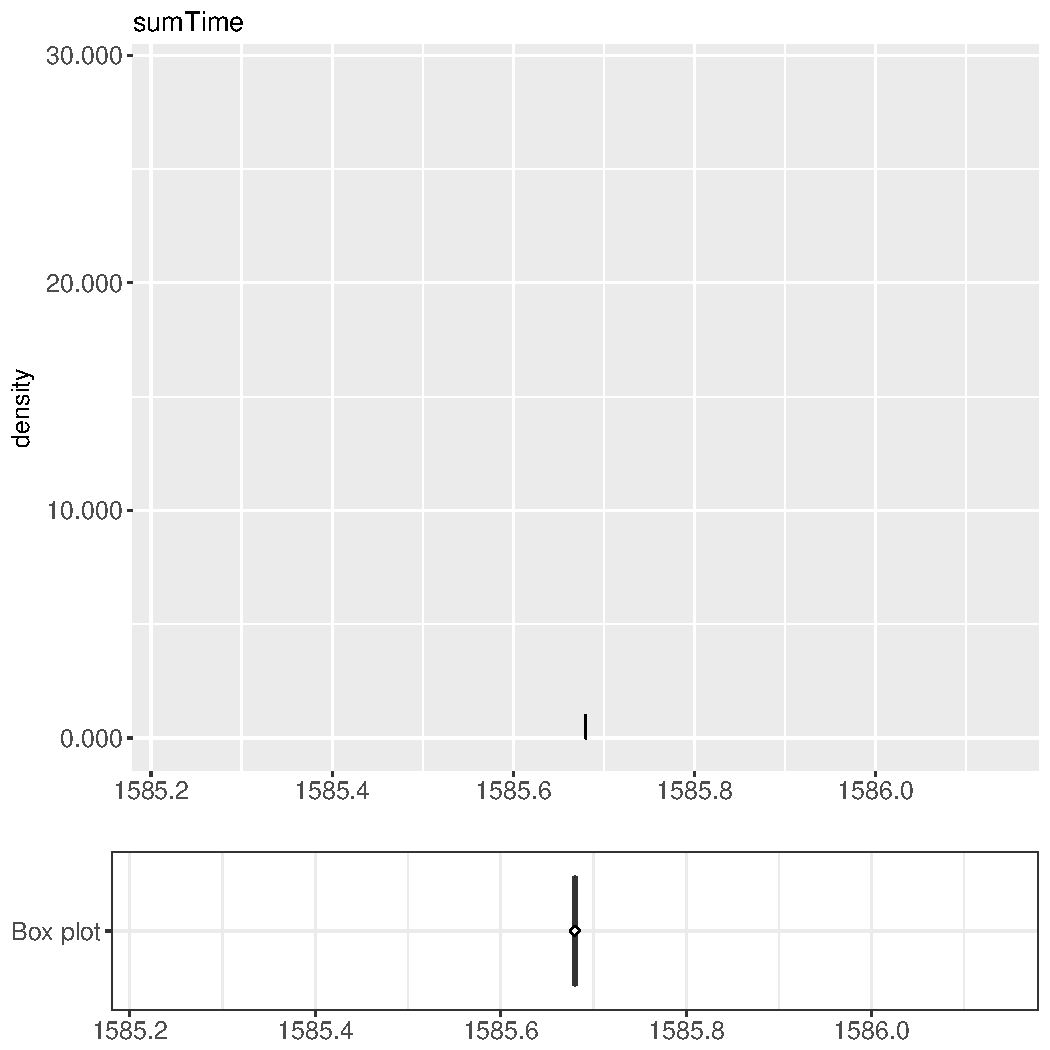
\includegraphics[width=\maxwidth]{figure/RH1_cashew_crime-1} 

\end{knitrout}
 \textbf{Total time for No cache}
\begin{knitrout}
\definecolor{shadecolor}{rgb}{0.969, 0.969, 0.969}\color{fgcolor}\begin{kframe}
\begin{verbatim}
## [1] "Sample size:  1"
##    Min. 1st Qu.  Median    Mean 3rd Qu.    Max. 
##    4311    4311    4311    4311    4311    4311
\end{verbatim}


{\ttfamily\noindent\bfseries\color{errorcolor}{\#\# Error in shapiro.test(subset(json\_data, treatment == "{}nocache"{} \& object == : sample size must be between 3 and 5000}}\end{kframe}
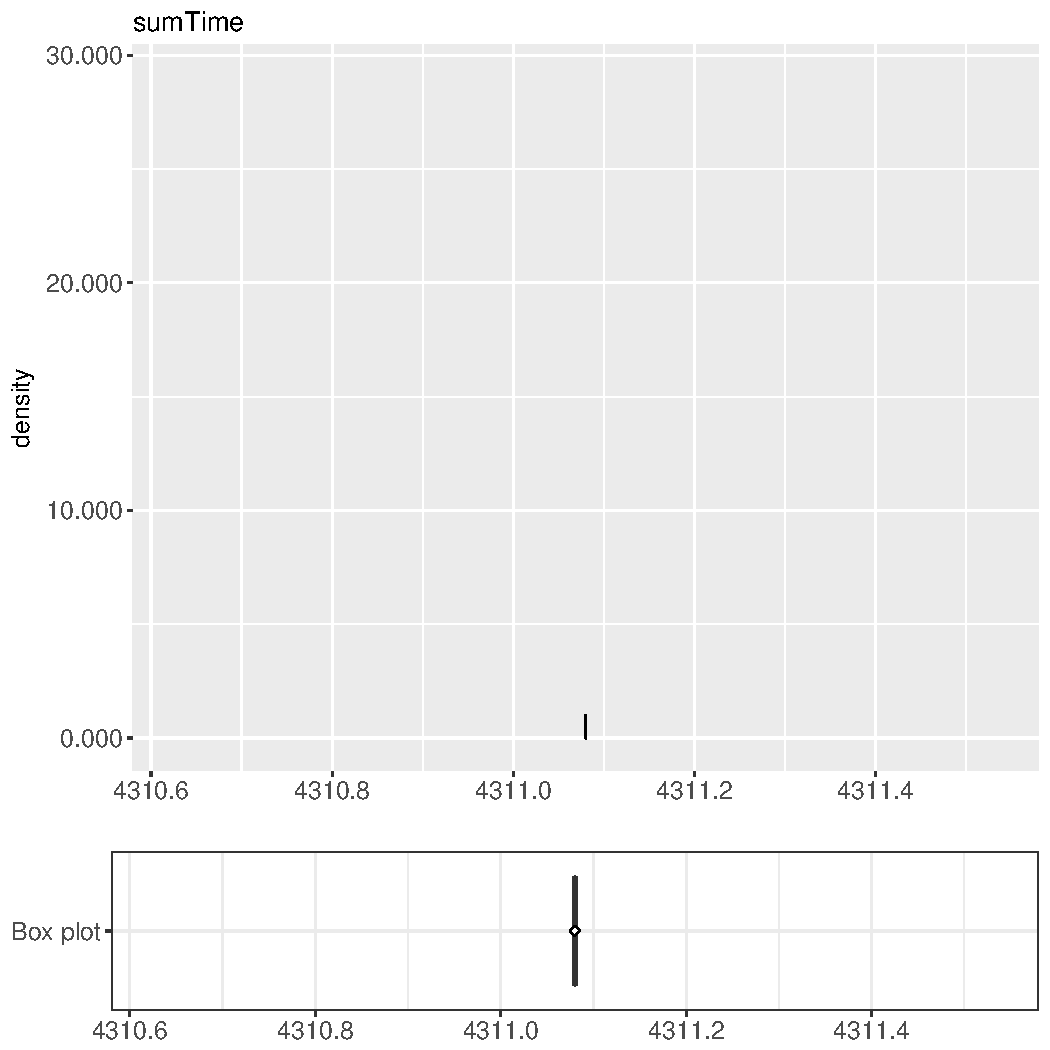
\includegraphics[width=\maxwidth]{figure/RH1_nocache_crime-1} 

\end{knitrout}
  
 \textbf{Comparison}
  
\begin{knitrout}
\definecolor{shadecolor}{rgb}{0.969, 0.969, 0.969}\color{fgcolor}
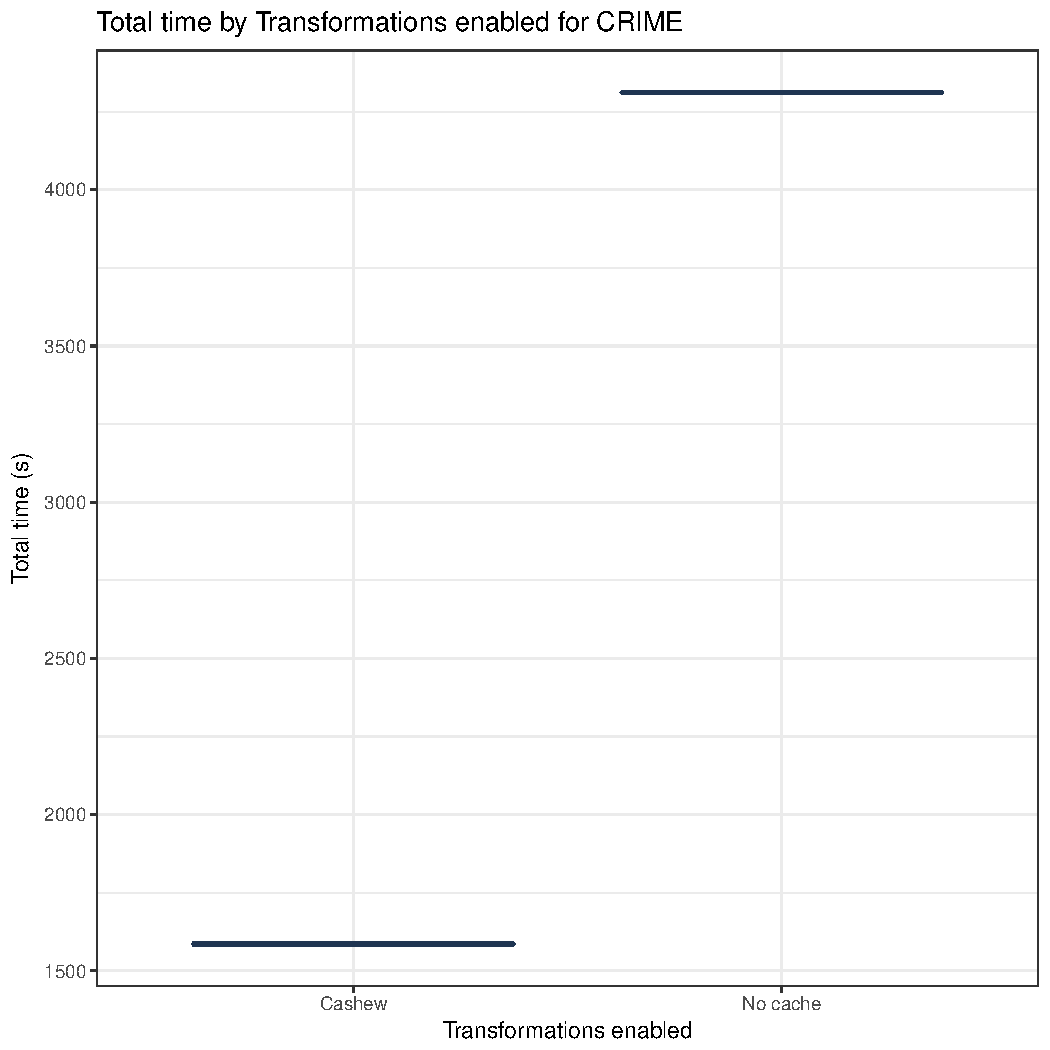
\includegraphics[width=\maxwidth]{figure/RH1_crime-1} 
\begin{kframe}

{\ttfamily\noindent\bfseries\color{errorcolor}{\#\# Error in eval(expr, envir, enclos): object 'shap\_cashew\_crime' not found}}\begin{verbatim}
## [1] ""
## [1] "Means comparison"
## [1] "Mean Total time for Cashew:  1585.68"
## [1] "Mean Total time for No cache:  4311.08"
## [1] "Absolute difference:  2725.4"
## Total time for No cache is  171.875788305333 % greater than 
## Total time for Cashew
\end{verbatim}
\end{kframe}
\end{knitrout}


 

	
	\subsubsection{RH1 Results: Total time Cashew = No cache}
	
	
	\begin{table}[H]
	\centering
	\caption{RH1 Results per Object}
	\begin{tabular}{ll}
	\textbf{Password1} & Inconclusive \\
	\textbf{Password2} & Inconclusive \\
	\textbf{Obscure} & Inconclusive \\
	\textbf{CRIME} & Inconclusive \\
	\end{tabular}
	\end{table}

	\begin{table}[H]
	\centering
	\caption{RH1 Results Summary}
	\begin{tabular}{ll}
	\textbf{Cashew \textless{} No cache:}& 0\% \\
	\textbf{Cashew \textgreater{} No cache:}& 0\%\\
	\textbf{Cashew:} & 0\%\\
	\textbf{No cache:} & 0\%\\
	\textbf{None:}& 0\%\\
	\textbf{Inconclusive:}& 100\%
			
	
	\end{tabular}
	\end{table}
	
	
	



\subsection{RH2: Total time for Cashew is equals than Total time for No Normalization}


 
\begin{knitrout}
\definecolor{shadecolor}{rgb}{0.969, 0.969, 0.969}\color{fgcolor}
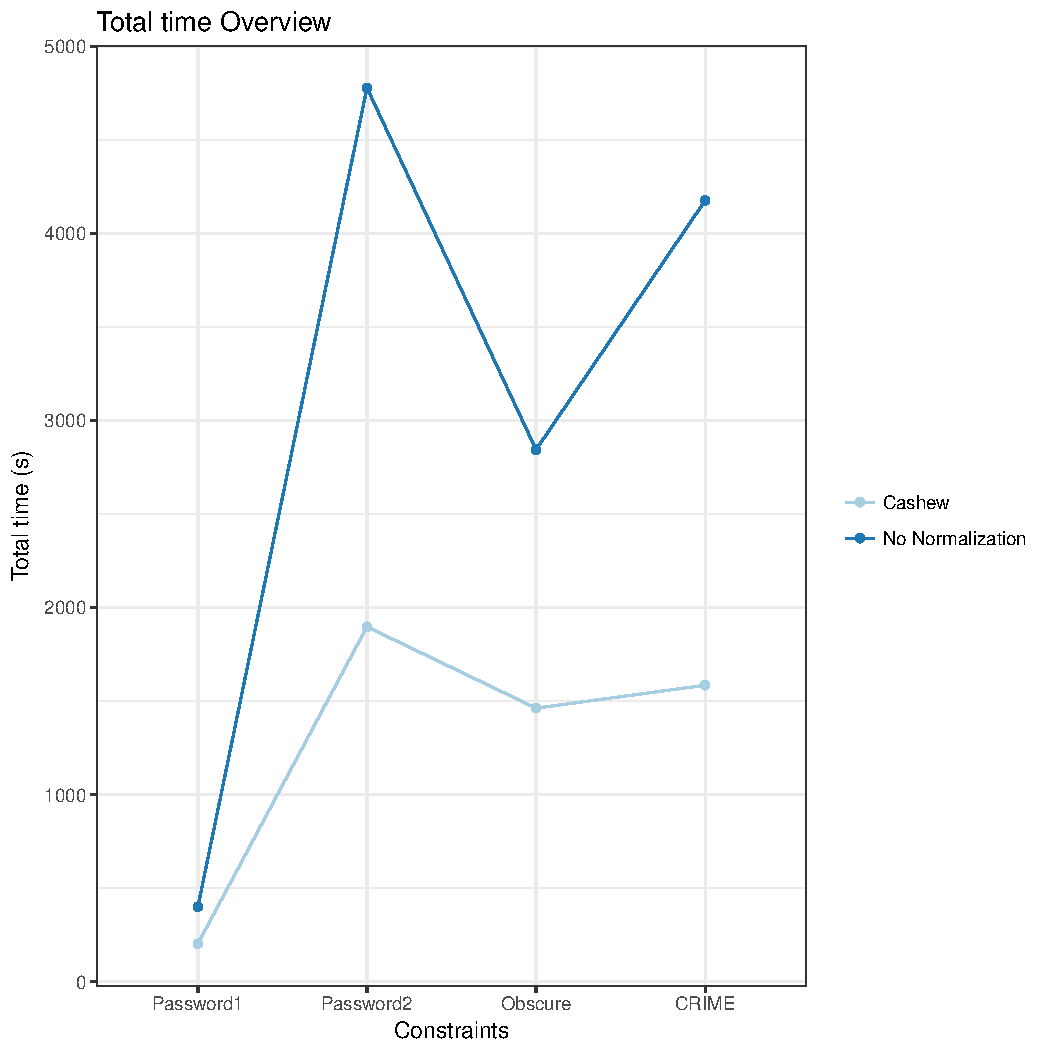
\includegraphics[width=\maxwidth]{figure/overview_RH2-1} 

\end{knitrout}
 	

\subsubsection{RH2.1: Object Password1}

 \textbf{Total time for Cashew}
\begin{knitrout}
\definecolor{shadecolor}{rgb}{0.969, 0.969, 0.969}\color{fgcolor}\begin{kframe}
\begin{verbatim}
## [1] "Sample size:  1"
##    Min. 1st Qu.  Median    Mean 3rd Qu.    Max. 
##   203.9   203.9   203.9   203.9   203.9   203.9
\end{verbatim}


{\ttfamily\noindent\bfseries\color{errorcolor}{\#\# Error in shapiro.test(subset(json\_data, treatment == "{}cashew"{} \& object == : sample size must be between 3 and 5000}}\end{kframe}
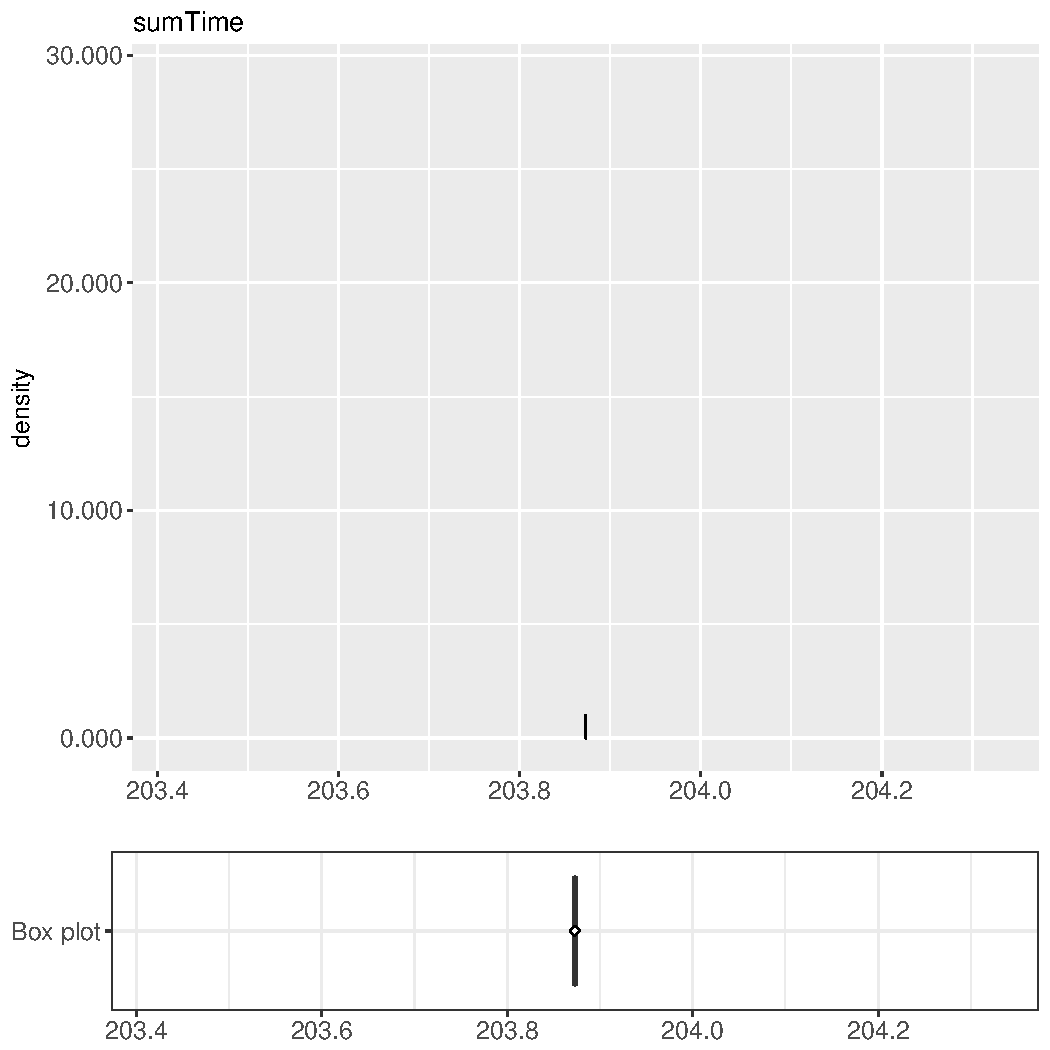
\includegraphics[width=\maxwidth]{figure/RH2_cashew_password-1} 

\end{knitrout}
 \textbf{Total time for No Normalization}
\begin{knitrout}
\definecolor{shadecolor}{rgb}{0.969, 0.969, 0.969}\color{fgcolor}\begin{kframe}
\begin{verbatim}
## [1] "Sample size:  1"
##    Min. 1st Qu.  Median    Mean 3rd Qu.    Max. 
##   401.7   401.7   401.7   401.7   401.7   401.7
\end{verbatim}


{\ttfamily\noindent\bfseries\color{errorcolor}{\#\# Error in shapiro.test(subset(json\_data, treatment == "{}trivialcaching"{} \& : sample size must be between 3 and 5000}}\end{kframe}
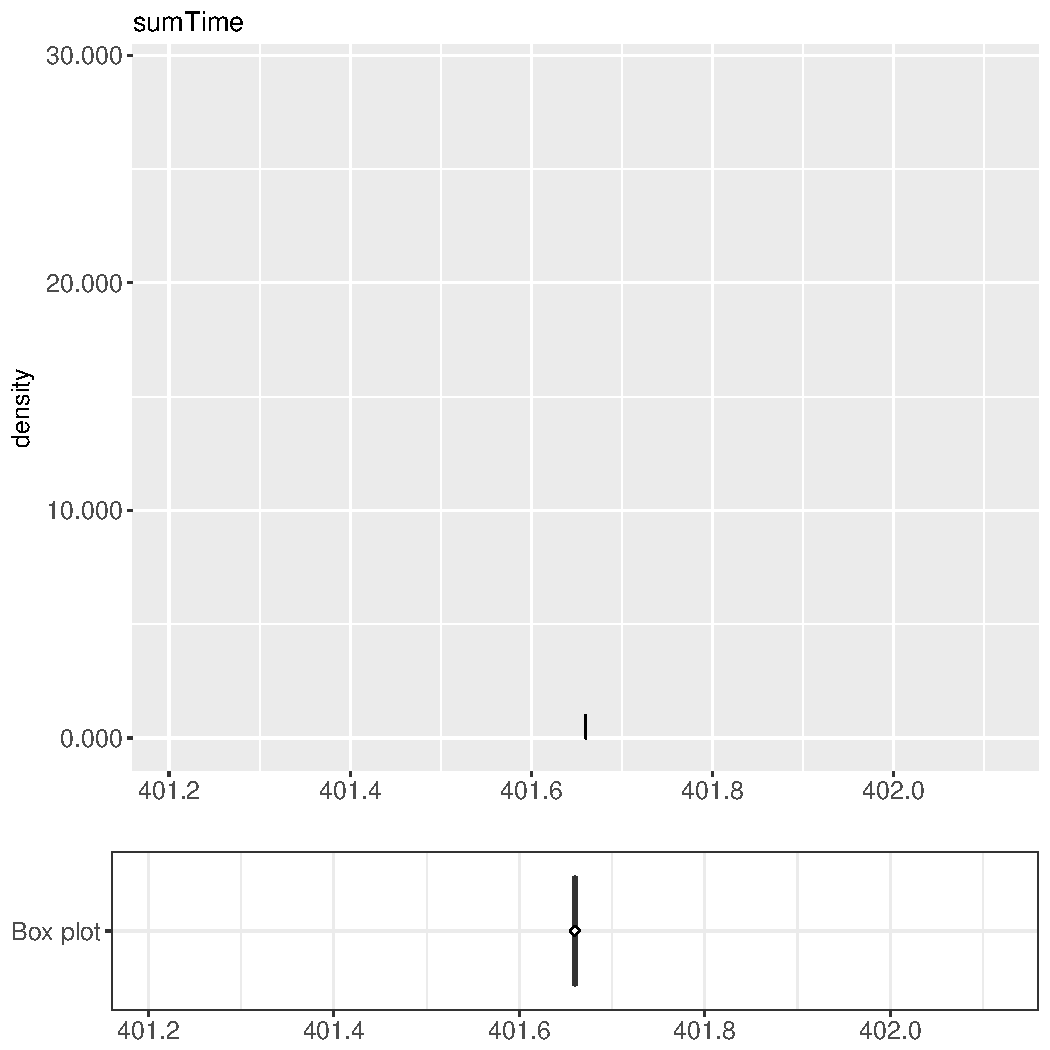
\includegraphics[width=\maxwidth]{figure/RH2_trivialcaching_password-1} 

\end{knitrout}
  
 \textbf{Comparison}
  
\begin{knitrout}
\definecolor{shadecolor}{rgb}{0.969, 0.969, 0.969}\color{fgcolor}
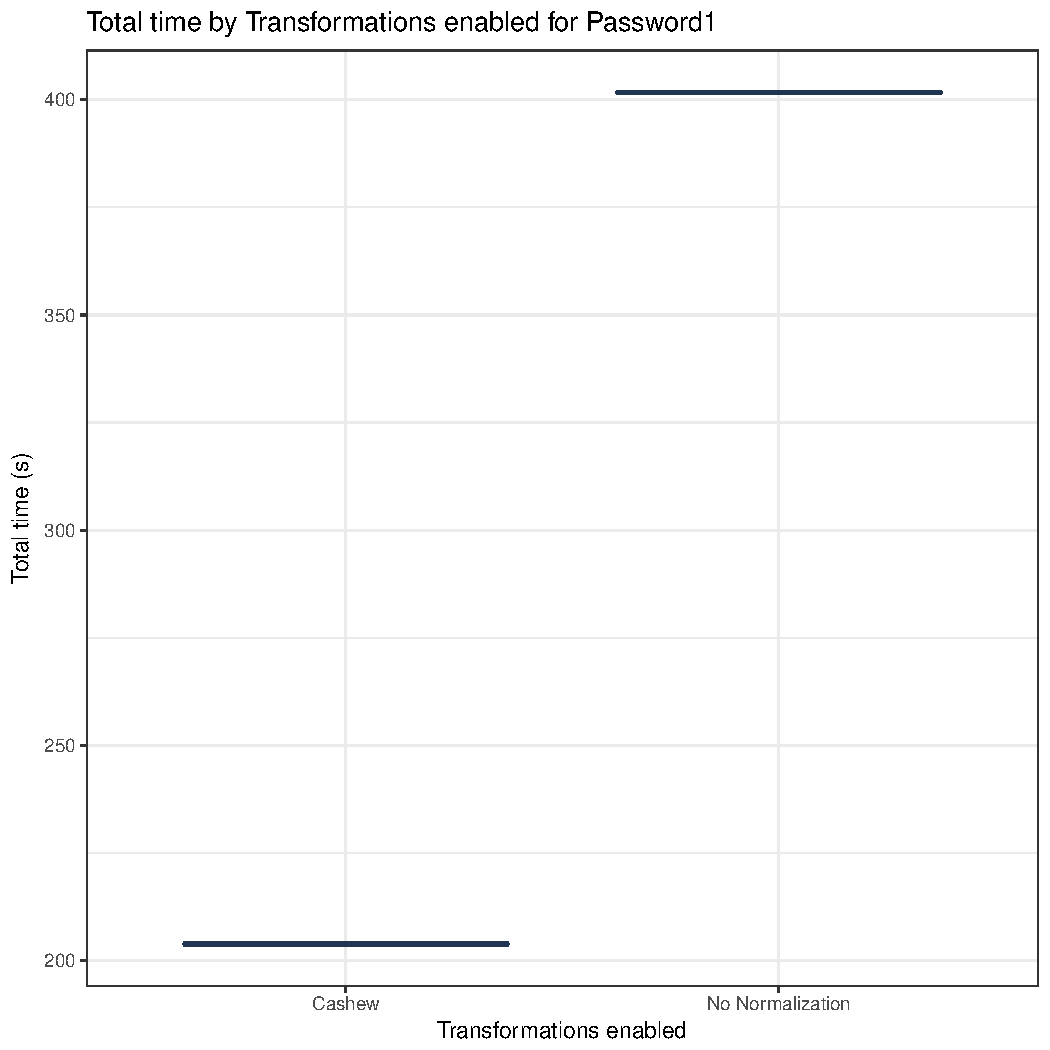
\includegraphics[width=\maxwidth]{figure/RH2_password-1} 
\begin{kframe}

{\ttfamily\noindent\bfseries\color{errorcolor}{\#\# Error in eval(expr, envir, enclos): object 'shap\_cashew\_password' not found}}\begin{verbatim}
## [1] ""
## [1] "Means comparison"
## [1] "Mean Total time for Cashew:  203.873"
## [1] "Mean Total time for No Normalization:  401.66"
## [1] "Absolute difference:  197.787"
## Total time for No Normalization is  97.0148082384622 % greater than 
## Total time for Cashew
\end{verbatim}
\end{kframe}
\end{knitrout}


\subsubsection{RH2.2: Object Password2}

 \textbf{Total time for Cashew}
\begin{knitrout}
\definecolor{shadecolor}{rgb}{0.969, 0.969, 0.969}\color{fgcolor}\begin{kframe}
\begin{verbatim}
## [1] "Sample size:  1"
##    Min. 1st Qu.  Median    Mean 3rd Qu.    Max. 
##    1898    1898    1898    1898    1898    1898
\end{verbatim}


{\ttfamily\noindent\bfseries\color{errorcolor}{\#\# Error in shapiro.test(subset(json\_data, treatment == "{}cashew"{} \& object == : sample size must be between 3 and 5000}}\end{kframe}
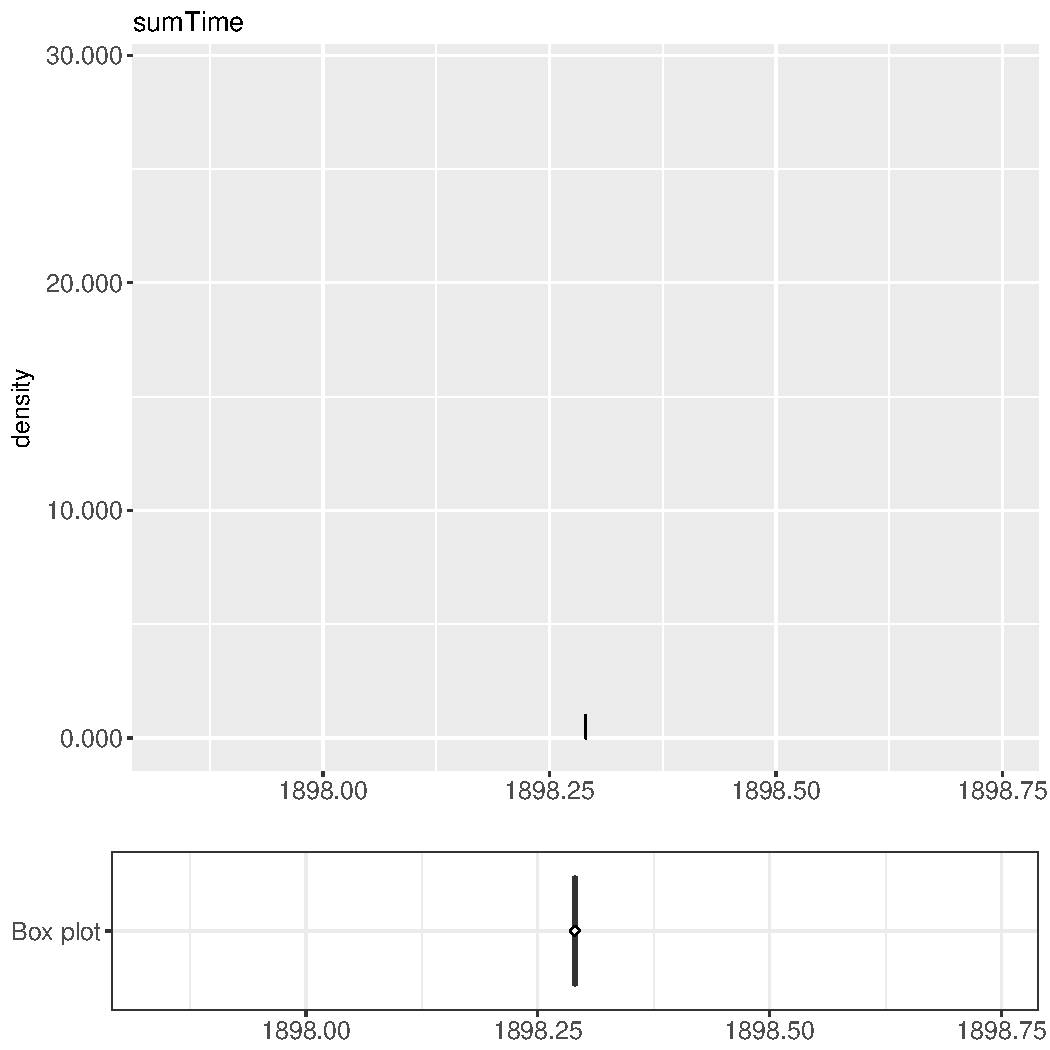
\includegraphics[width=\maxwidth]{figure/RH2_cashew_password2-1} 

\end{knitrout}
 \textbf{Total time for No Normalization}
\begin{knitrout}
\definecolor{shadecolor}{rgb}{0.969, 0.969, 0.969}\color{fgcolor}\begin{kframe}
\begin{verbatim}
## [1] "Sample size:  1"
##    Min. 1st Qu.  Median    Mean 3rd Qu.    Max. 
##    4779    4779    4779    4779    4779    4779
\end{verbatim}


{\ttfamily\noindent\bfseries\color{errorcolor}{\#\# Error in shapiro.test(subset(json\_data, treatment == "{}trivialcaching"{} \& : sample size must be between 3 and 5000}}\end{kframe}
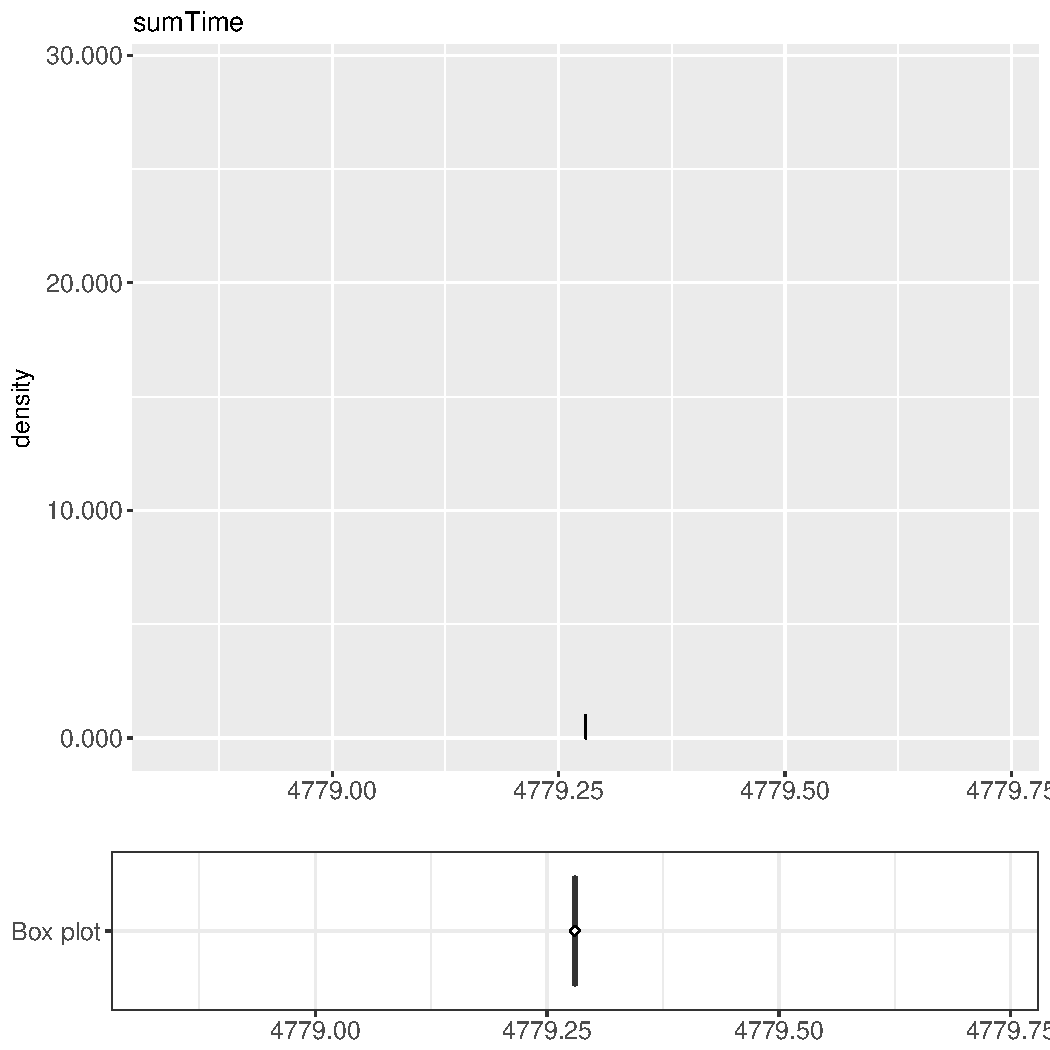
\includegraphics[width=\maxwidth]{figure/RH2_trivialcaching_password2-1} 

\end{knitrout}
  
 \textbf{Comparison}
  
\begin{knitrout}
\definecolor{shadecolor}{rgb}{0.969, 0.969, 0.969}\color{fgcolor}
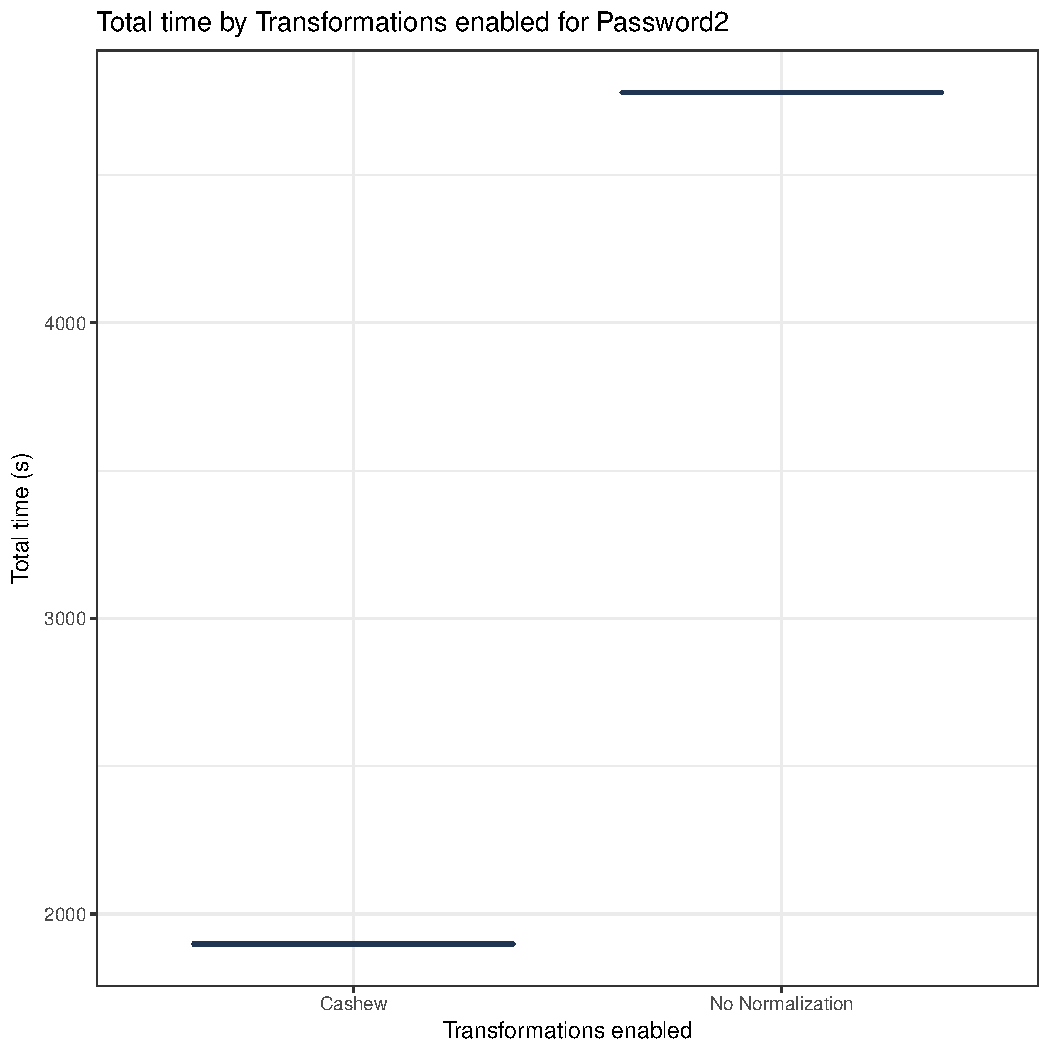
\includegraphics[width=\maxwidth]{figure/RH2_password2-1} 
\begin{kframe}

{\ttfamily\noindent\bfseries\color{errorcolor}{\#\# Error in eval(expr, envir, enclos): object 'shap\_cashew\_password2' not found}}\begin{verbatim}
## [1] ""
## [1] "Means comparison"
## [1] "Mean Total time for Cashew:  1898.29"
## [1] "Mean Total time for No Normalization:  4779.28"
## [1] "Absolute difference:  2880.99"
## Total time for No Normalization is  151.767643510739 % greater than 
## Total time for Cashew
\end{verbatim}
\end{kframe}
\end{knitrout}


\subsubsection{RH2.3: Object Obscure}

 \textbf{Total time for Cashew}
\begin{knitrout}
\definecolor{shadecolor}{rgb}{0.969, 0.969, 0.969}\color{fgcolor}\begin{kframe}
\begin{verbatim}
## [1] "Sample size:  1"
##    Min. 1st Qu.  Median    Mean 3rd Qu.    Max. 
##    1463    1463    1463    1463    1463    1463
\end{verbatim}


{\ttfamily\noindent\bfseries\color{errorcolor}{\#\# Error in shapiro.test(subset(json\_data, treatment == "{}cashew"{} \& object == : sample size must be between 3 and 5000}}\end{kframe}
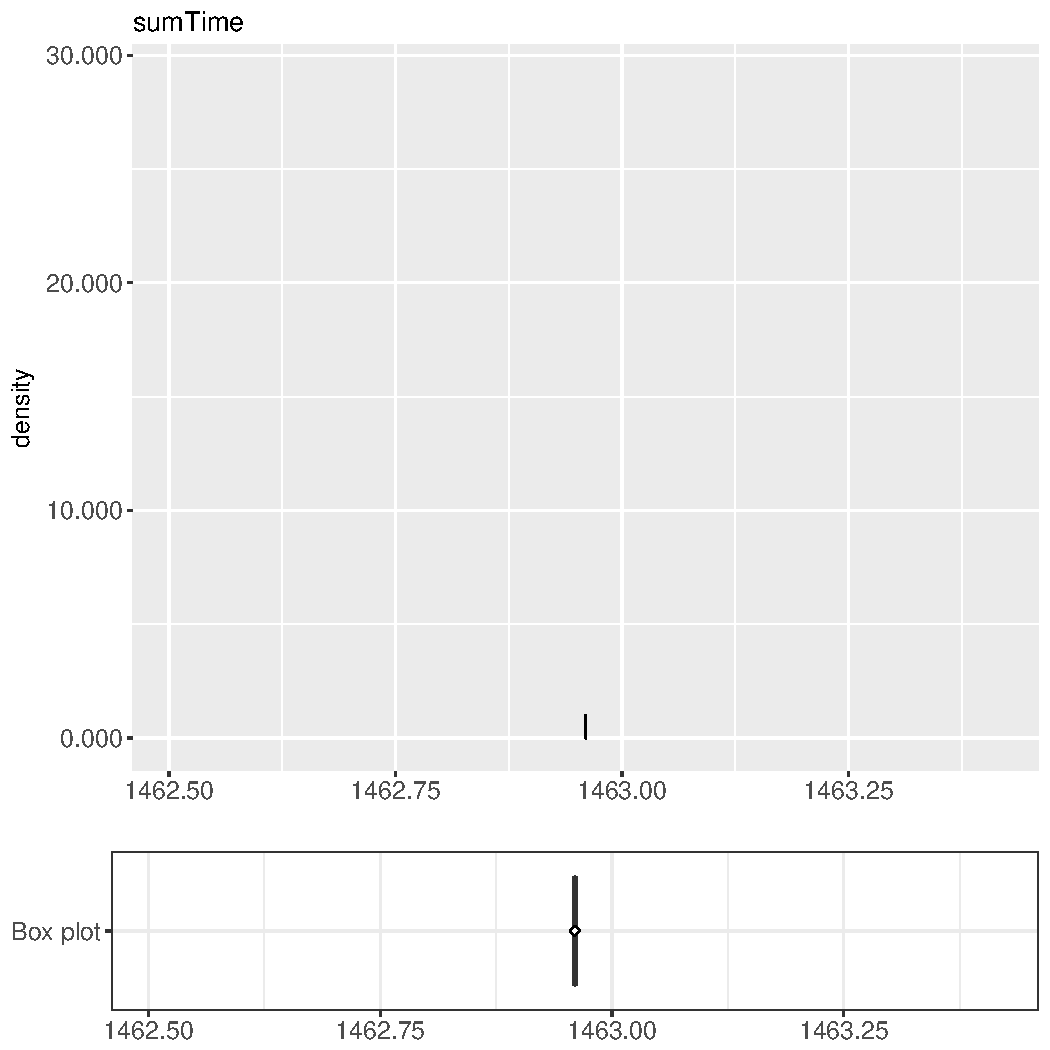
\includegraphics[width=\maxwidth]{figure/RH2_cashew_obscure-1} 

\end{knitrout}
 \textbf{Total time for No Normalization}
\begin{knitrout}
\definecolor{shadecolor}{rgb}{0.969, 0.969, 0.969}\color{fgcolor}\begin{kframe}
\begin{verbatim}
## [1] "Sample size:  1"
##    Min. 1st Qu.  Median    Mean 3rd Qu.    Max. 
##    2845    2845    2845    2845    2845    2845
\end{verbatim}


{\ttfamily\noindent\bfseries\color{errorcolor}{\#\# Error in shapiro.test(subset(json\_data, treatment == "{}trivialcaching"{} \& : sample size must be between 3 and 5000}}\end{kframe}
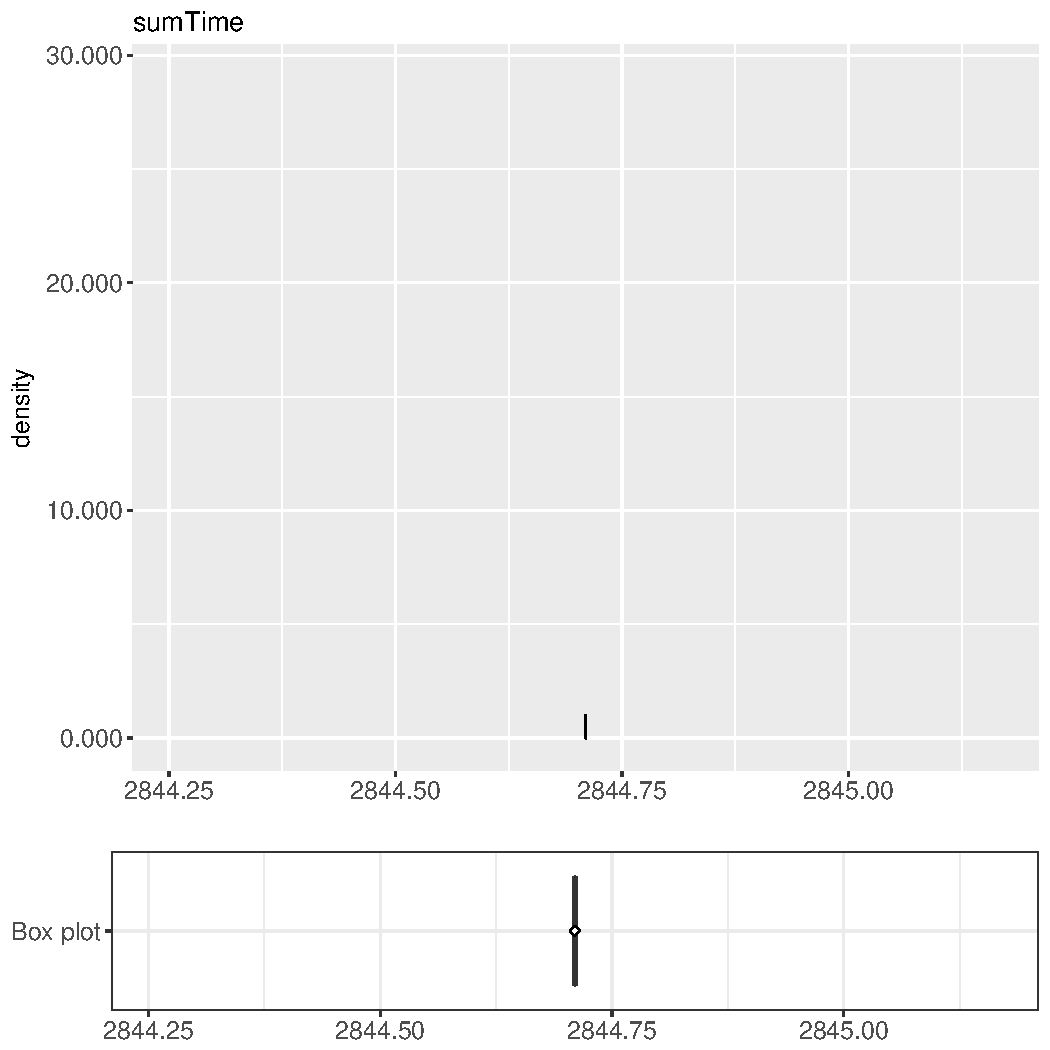
\includegraphics[width=\maxwidth]{figure/RH2_trivialcaching_obscure-1} 

\end{knitrout}
  
 \textbf{Comparison}
  
\begin{knitrout}
\definecolor{shadecolor}{rgb}{0.969, 0.969, 0.969}\color{fgcolor}
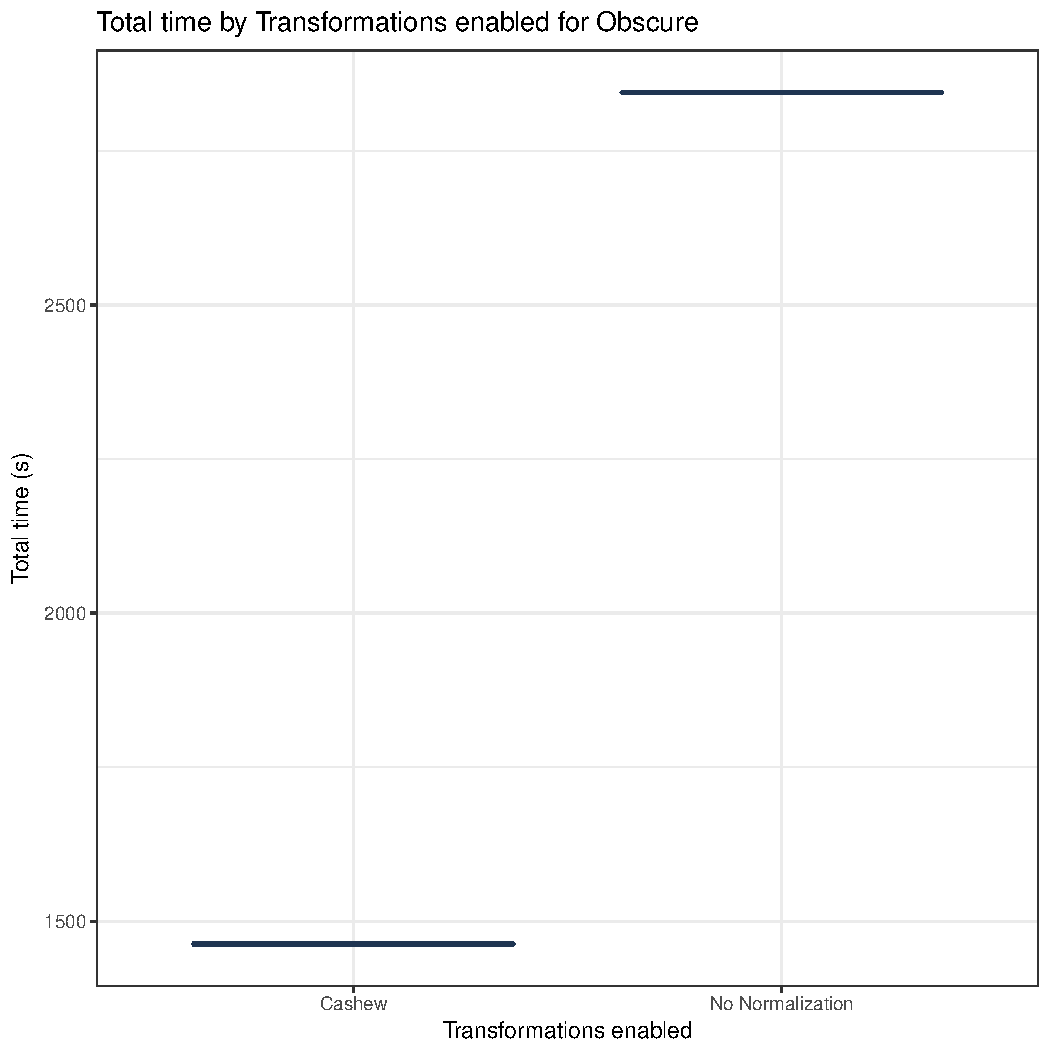
\includegraphics[width=\maxwidth]{figure/RH2_obscure-1} 
\begin{kframe}

{\ttfamily\noindent\bfseries\color{errorcolor}{\#\# Error in eval(expr, envir, enclos): object 'shap\_cashew\_obscure' not found}}\begin{verbatim}
## [1] ""
## [1] "Means comparison"
## [1] "Mean Total time for Cashew:  1462.96"
## [1] "Mean Total time for No Normalization:  2844.71"
## [1] "Absolute difference:  1381.75"
## Total time for No Normalization is  94.4489254661782 % greater than 
## Total time for Cashew
\end{verbatim}
\end{kframe}
\end{knitrout}


\subsubsection{RH2.4: Object CRIME}

 \textbf{Total time for Cashew}
\begin{knitrout}
\definecolor{shadecolor}{rgb}{0.969, 0.969, 0.969}\color{fgcolor}\begin{kframe}
\begin{verbatim}
## [1] "Sample size:  1"
##    Min. 1st Qu.  Median    Mean 3rd Qu.    Max. 
##    1586    1586    1586    1586    1586    1586
\end{verbatim}


{\ttfamily\noindent\bfseries\color{errorcolor}{\#\# Error in shapiro.test(subset(json\_data, treatment == "{}cashew"{} \& object == : sample size must be between 3 and 5000}}\end{kframe}
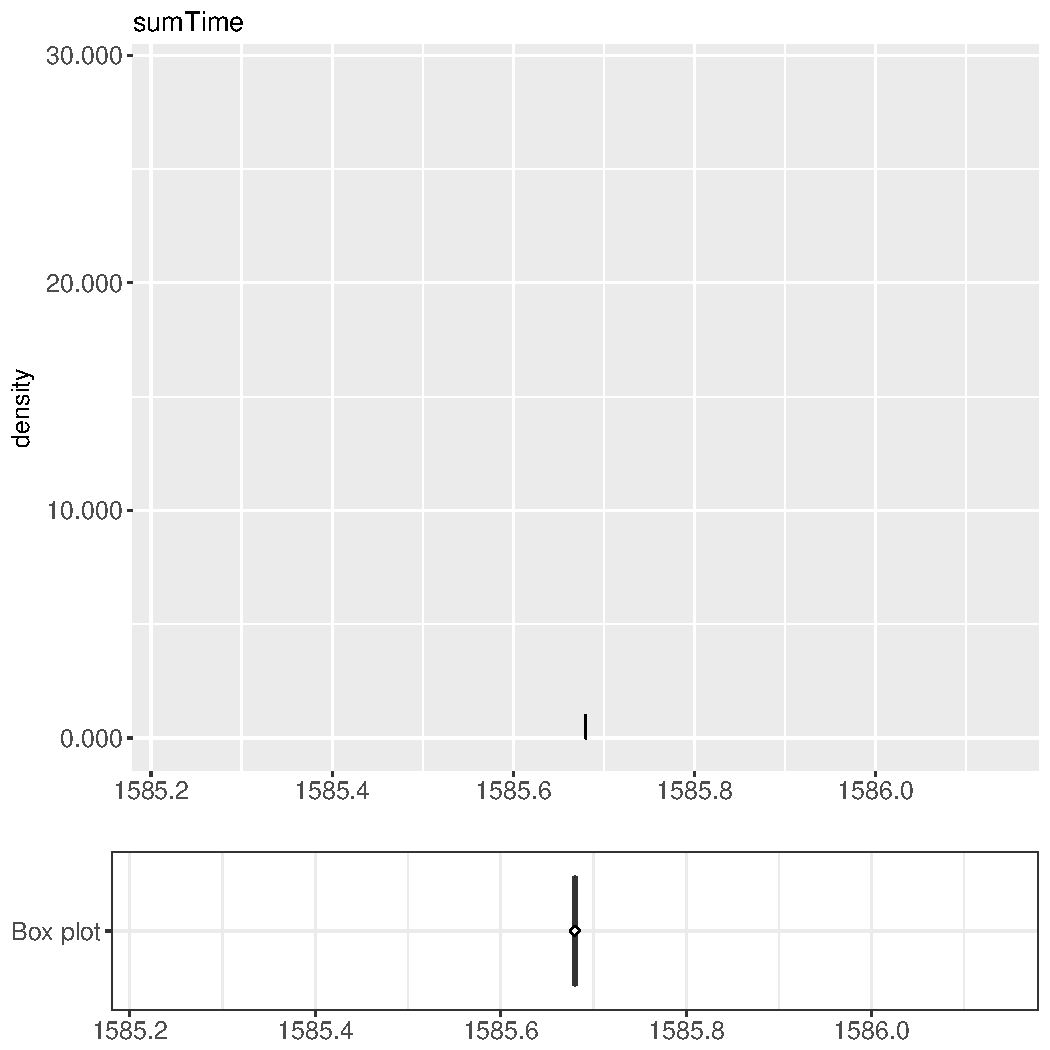
\includegraphics[width=\maxwidth]{figure/RH2_cashew_crime-1} 

\end{knitrout}
 \textbf{Total time for No Normalization}
\begin{knitrout}
\definecolor{shadecolor}{rgb}{0.969, 0.969, 0.969}\color{fgcolor}\begin{kframe}
\begin{verbatim}
## [1] "Sample size:  1"
##    Min. 1st Qu.  Median    Mean 3rd Qu.    Max. 
##    4177    4177    4177    4177    4177    4177
\end{verbatim}


{\ttfamily\noindent\bfseries\color{errorcolor}{\#\# Error in shapiro.test(subset(json\_data, treatment == "{}trivialcaching"{} \& : sample size must be between 3 and 5000}}\end{kframe}
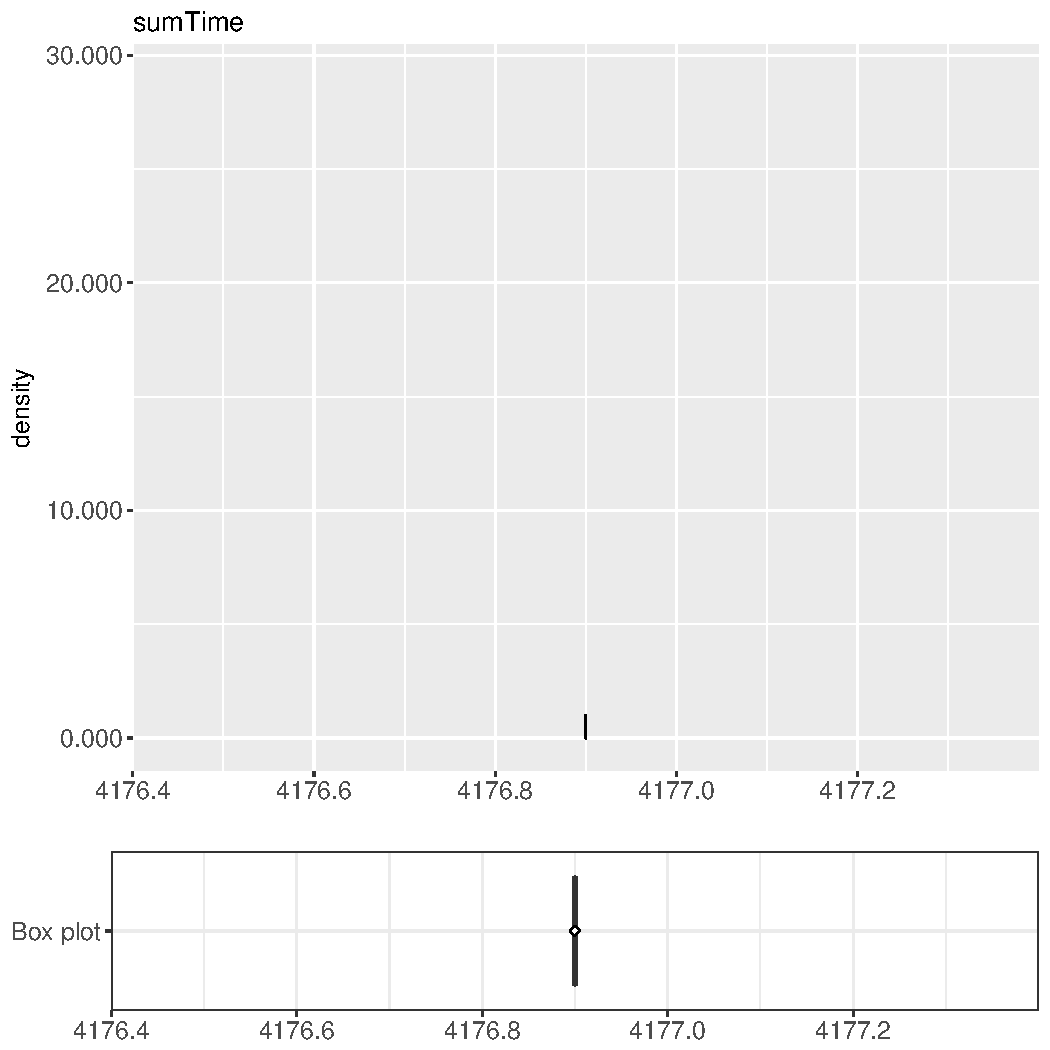
\includegraphics[width=\maxwidth]{figure/RH2_trivialcaching_crime-1} 

\end{knitrout}
  
 \textbf{Comparison}
  
\begin{knitrout}
\definecolor{shadecolor}{rgb}{0.969, 0.969, 0.969}\color{fgcolor}
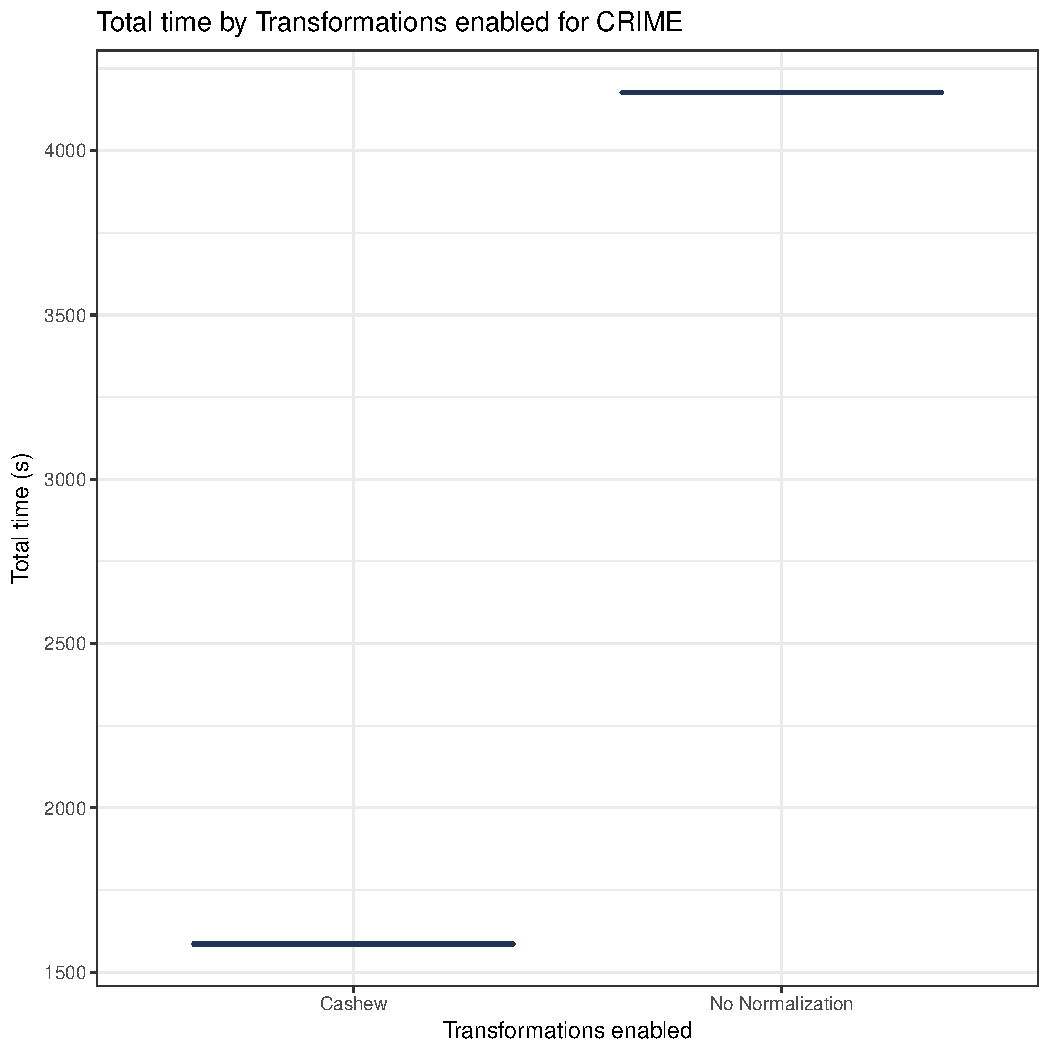
\includegraphics[width=\maxwidth]{figure/RH2_crime-1} 
\begin{kframe}

{\ttfamily\noindent\bfseries\color{errorcolor}{\#\# Error in eval(expr, envir, enclos): object 'shap\_cashew\_crime' not found}}\begin{verbatim}
## [1] ""
## [1] "Means comparison"
## [1] "Mean Total time for Cashew:  1585.68"
## [1] "Mean Total time for No Normalization:  4176.9"
## [1] "Absolute difference:  2591.22"
## Total time for No Normalization is  163.413803541698 % greater than 
## Total time for Cashew
\end{verbatim}
\end{kframe}
\end{knitrout}


 

	
	\subsubsection{RH2 Results: Total time Cashew = No Normalization}
	
	
	\begin{table}[H]
	\centering
	\caption{RH2 Results per Object}
	\begin{tabular}{ll}
	\textbf{Password1} & Inconclusive \\
	\textbf{Password2} & Inconclusive \\
	\textbf{Obscure} & Inconclusive \\
	\textbf{CRIME} & Inconclusive \\
	\end{tabular}
	\end{table}

	\begin{table}[H]
	\centering
	\caption{RH2 Results Summary}
	\begin{tabular}{ll}
	\textbf{Cashew \textless{} No Normalization:}& 0\% \\
	\textbf{Cashew \textgreater{} No Normalization:}& 0\%\\
	\textbf{Cashew:} & 0\%\\
	\textbf{No Normalization:} & 0\%\\
	\textbf{None:}& 0\%\\
	\textbf{Inconclusive:}& 100\%
			
	
	\end{tabular}
	\end{table}
	
	
	



\subsection{RH3: Number of hits for Cashew is equals than Number of hits for No Normalization}


 
\begin{knitrout}
\definecolor{shadecolor}{rgb}{0.969, 0.969, 0.969}\color{fgcolor}
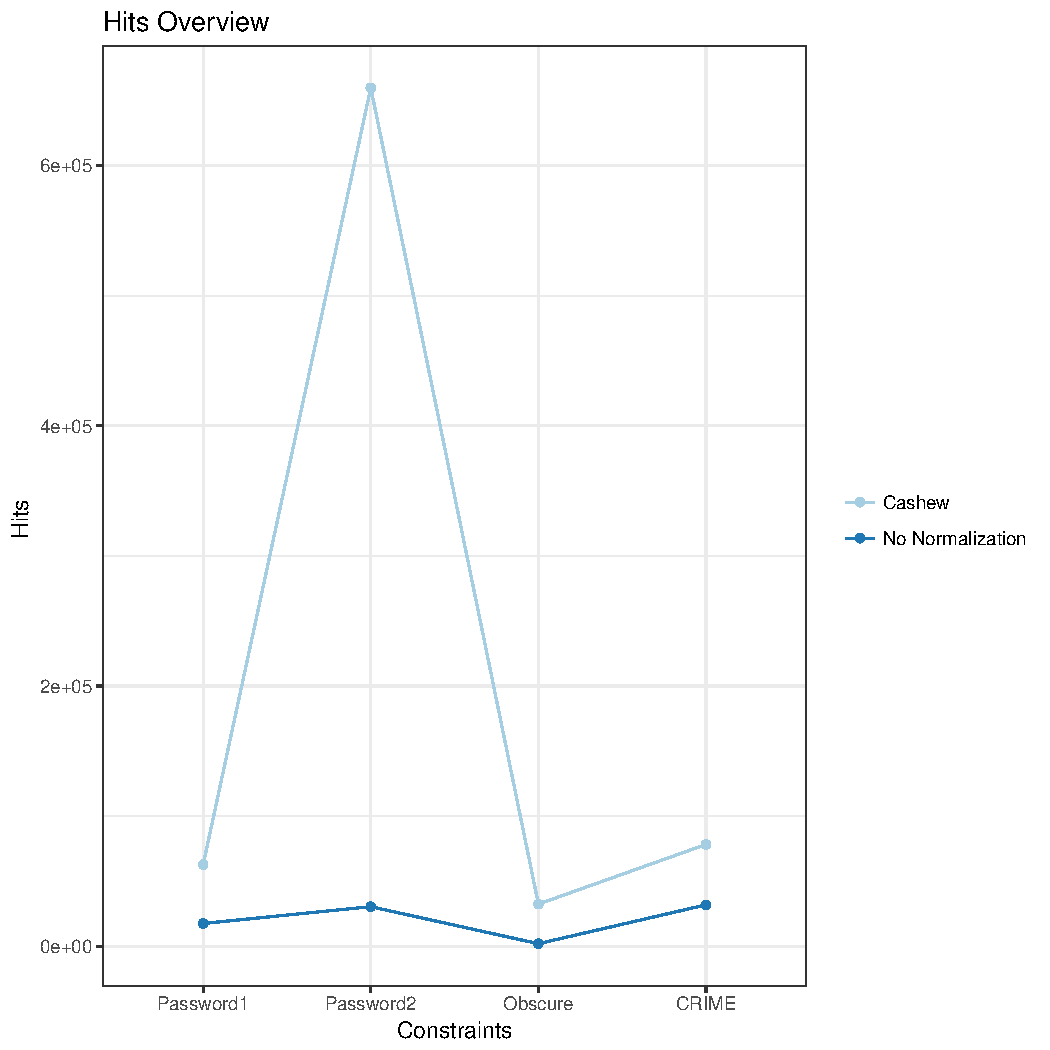
\includegraphics[width=\maxwidth]{figure/overview_RH3-1} 

\end{knitrout}
 	

\subsubsection{RH3.1: Object Password1}

 \textbf{Hits for Cashew}
\begin{knitrout}
\definecolor{shadecolor}{rgb}{0.969, 0.969, 0.969}\color{fgcolor}\begin{kframe}
\begin{verbatim}
## [1] "Sample size:  1"
##    Min. 1st Qu.  Median    Mean 3rd Qu.    Max. 
##   62800   62800   62800   62800   62800   62800
\end{verbatim}


{\ttfamily\noindent\bfseries\color{errorcolor}{\#\# Error in shapiro.test(subset(json\_data, treatment == "{}cashew"{} \& object == : sample size must be between 3 and 5000}}\end{kframe}
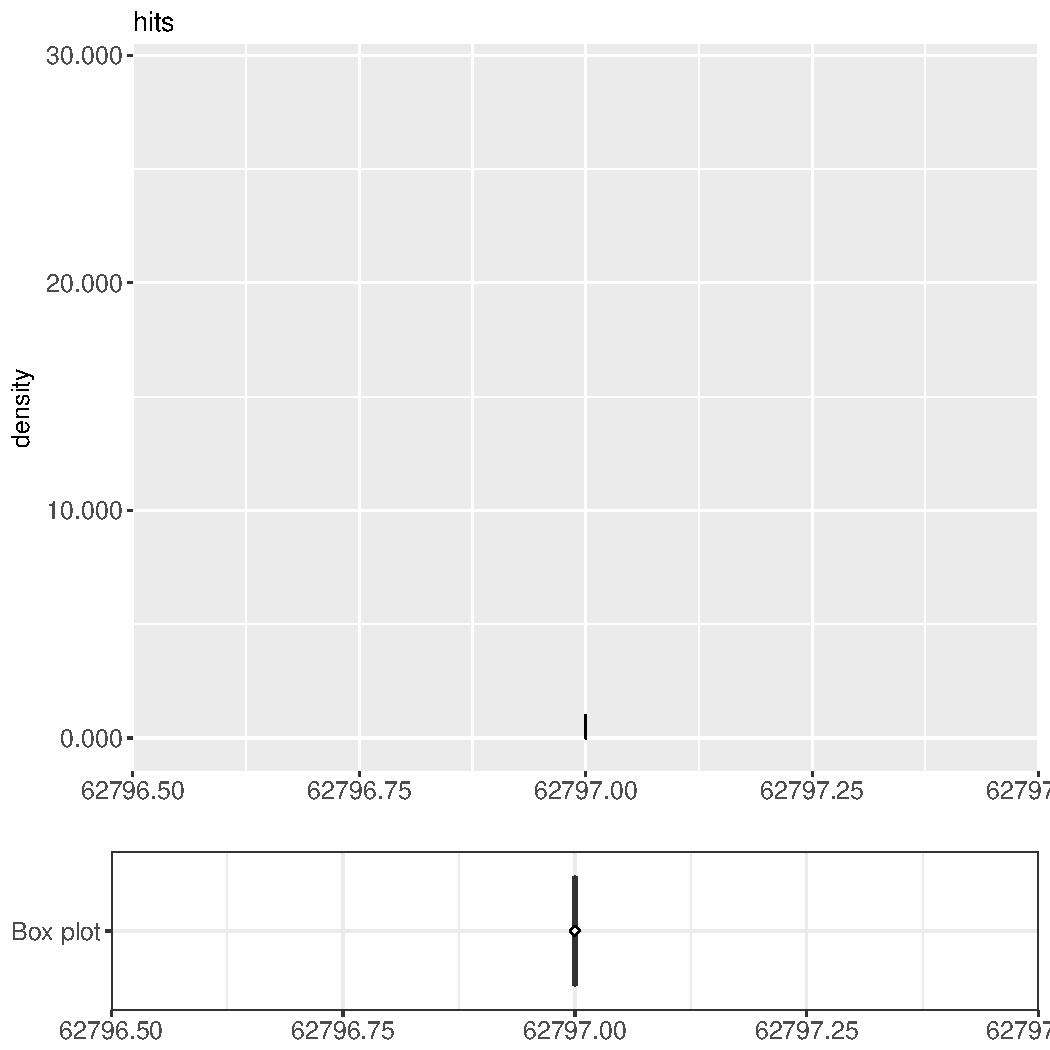
\includegraphics[width=\maxwidth]{figure/RH3_cashew_password-1} 

\end{knitrout}
 \textbf{Hits for No Normalization}
\begin{knitrout}
\definecolor{shadecolor}{rgb}{0.969, 0.969, 0.969}\color{fgcolor}\begin{kframe}
\begin{verbatim}
## [1] "Sample size:  1"
##    Min. 1st Qu.  Median    Mean 3rd Qu.    Max. 
##   17550   17550   17550   17550   17550   17550
\end{verbatim}


{\ttfamily\noindent\bfseries\color{errorcolor}{\#\# Error in shapiro.test(subset(json\_data, treatment == "{}trivialcaching"{} \& : sample size must be between 3 and 5000}}\end{kframe}
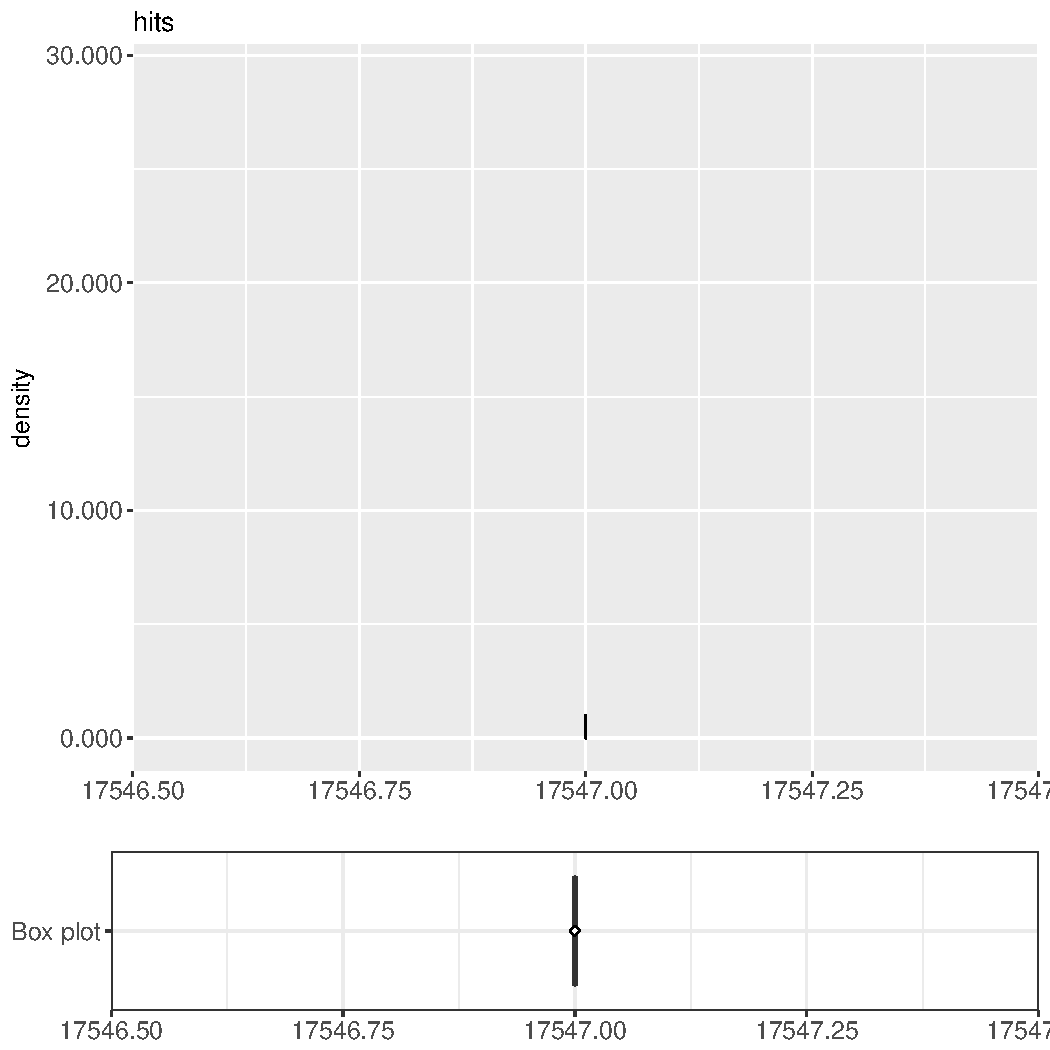
\includegraphics[width=\maxwidth]{figure/RH3_trivialcaching_password-1} 

\end{knitrout}
  
 \textbf{Comparison}
  
\begin{knitrout}
\definecolor{shadecolor}{rgb}{0.969, 0.969, 0.969}\color{fgcolor}
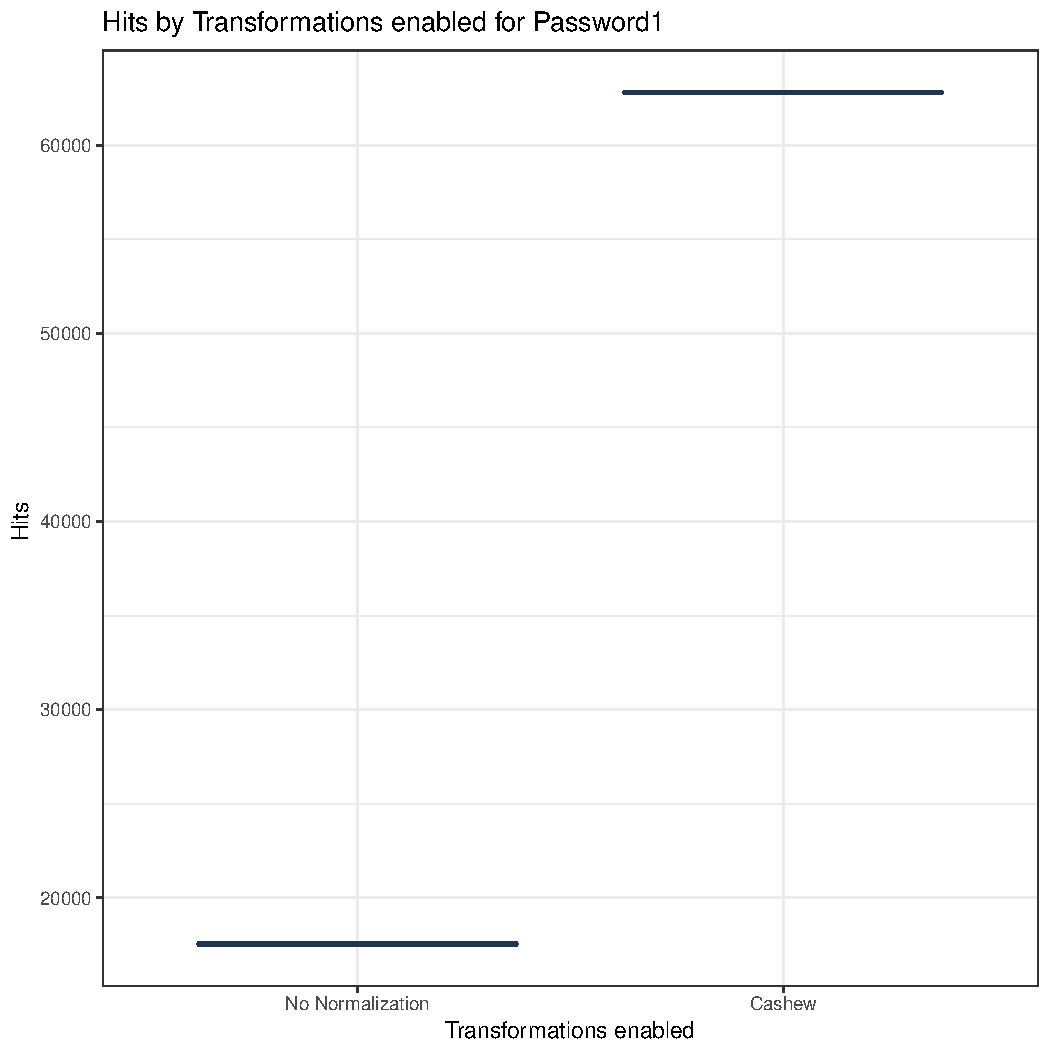
\includegraphics[width=\maxwidth]{figure/RH3_password-1} 
\begin{kframe}

{\ttfamily\noindent\bfseries\color{errorcolor}{\#\# Error in eval(expr, envir, enclos): object 'shap\_cashew\_password' not found}}\begin{verbatim}
## [1] ""
## [1] "Means comparison"
## [1] "Mean Hits for Cashew:  62797"
## [1] "Mean Hits for No Normalization:  17547"
## [1] "Absolute difference:  45250"
## Hits for Cashew is  257.878839687696 % greater than 
##  Hits for No Normalization
\end{verbatim}
\end{kframe}
\end{knitrout}


\subsubsection{RH3.2: Object Password2}

 \textbf{Hits for Cashew}
\begin{knitrout}
\definecolor{shadecolor}{rgb}{0.969, 0.969, 0.969}\color{fgcolor}\begin{kframe}
\begin{verbatim}
## [1] "Sample size:  1"
##    Min. 1st Qu.  Median    Mean 3rd Qu.    Max. 
##  659800  659800  659800  659800  659800  659800
\end{verbatim}


{\ttfamily\noindent\bfseries\color{errorcolor}{\#\# Error in shapiro.test(subset(json\_data, treatment == "{}cashew"{} \& object == : sample size must be between 3 and 5000}}\end{kframe}
\includegraphics[width=\maxwidth]{figure/RH3_cashew_password2-1} 

\end{knitrout}
 \textbf{Hits for No Normalization}
\begin{knitrout}
\definecolor{shadecolor}{rgb}{0.969, 0.969, 0.969}\color{fgcolor}\begin{kframe}
\begin{verbatim}
## [1] "Sample size:  1"
##    Min. 1st Qu.  Median    Mean 3rd Qu.    Max. 
##   30450   30450   30450   30450   30450   30450
\end{verbatim}


{\ttfamily\noindent\bfseries\color{errorcolor}{\#\# Error in shapiro.test(subset(json\_data, treatment == "{}trivialcaching"{} \& : sample size must be between 3 and 5000}}\end{kframe}
\includegraphics[width=\maxwidth]{figure/RH3_trivialcaching_password2-1} 

\end{knitrout}
  
 \textbf{Comparison}
  
\begin{knitrout}
\definecolor{shadecolor}{rgb}{0.969, 0.969, 0.969}\color{fgcolor}
\includegraphics[width=\maxwidth]{figure/RH3_password2-1} 
\begin{kframe}

{\ttfamily\noindent\bfseries\color{errorcolor}{\#\# Error in eval(expr, envir, enclos): object 'shap\_cashew\_password2' not found}}\begin{verbatim}
## [1] ""
## [1] "Means comparison"
## [1] "Mean Hits for Cashew:  659804"
## [1] "Mean Hits for No Normalization:  30448"
## [1] "Absolute difference:  629356"
## Hits for Cashew is  2066.98633736206 % greater than 
##  Hits for No Normalization
\end{verbatim}
\end{kframe}
\end{knitrout}


\subsubsection{RH3.3: Object Obscure}

 \textbf{Hits for Cashew}
\begin{knitrout}
\definecolor{shadecolor}{rgb}{0.969, 0.969, 0.969}\color{fgcolor}\begin{kframe}
\begin{verbatim}
## [1] "Sample size:  1"
##    Min. 1st Qu.  Median    Mean 3rd Qu.    Max. 
##   32440   32440   32440   32440   32440   32440
\end{verbatim}


{\ttfamily\noindent\bfseries\color{errorcolor}{\#\# Error in shapiro.test(subset(json\_data, treatment == "{}cashew"{} \& object == : sample size must be between 3 and 5000}}\end{kframe}
\includegraphics[width=\maxwidth]{figure/RH3_cashew_obscure-1} 

\end{knitrout}
 \textbf{Hits for No Normalization}
\begin{knitrout}
\definecolor{shadecolor}{rgb}{0.969, 0.969, 0.969}\color{fgcolor}\begin{kframe}
\begin{verbatim}
## [1] "Sample size:  1"
##    Min. 1st Qu.  Median    Mean 3rd Qu.    Max. 
##    1999    1999    1999    1999    1999    1999
\end{verbatim}


{\ttfamily\noindent\bfseries\color{errorcolor}{\#\# Error in shapiro.test(subset(json\_data, treatment == "{}trivialcaching"{} \& : sample size must be between 3 and 5000}}\end{kframe}
\includegraphics[width=\maxwidth]{figure/RH3_trivialcaching_obscure-1} 

\end{knitrout}
  
 \textbf{Comparison}
  
\begin{knitrout}
\definecolor{shadecolor}{rgb}{0.969, 0.969, 0.969}\color{fgcolor}
\includegraphics[width=\maxwidth]{figure/RH3_obscure-1} 
\begin{kframe}

{\ttfamily\noindent\bfseries\color{errorcolor}{\#\# Error in eval(expr, envir, enclos): object 'shap\_cashew\_obscure' not found}}\begin{verbatim}
## [1] ""
## [1] "Means comparison"
## [1] "Mean Hits for Cashew:  32443"
## [1] "Mean Hits for No Normalization:  1999"
## [1] "Absolute difference:  30444"
## Hits for Cashew is  1522.96148074037 % greater than 
##  Hits for No Normalization
\end{verbatim}
\end{kframe}
\end{knitrout}


\subsubsection{RH3.4: Object CRIME}

 \textbf{Hits for Cashew}
\begin{knitrout}
\definecolor{shadecolor}{rgb}{0.969, 0.969, 0.969}\color{fgcolor}\begin{kframe}
\begin{verbatim}
## [1] "Sample size:  1"
##    Min. 1st Qu.  Median    Mean 3rd Qu.    Max. 
##   78290   78290   78290   78290   78290   78290
\end{verbatim}


{\ttfamily\noindent\bfseries\color{errorcolor}{\#\# Error in shapiro.test(subset(json\_data, treatment == "{}cashew"{} \& object == : sample size must be between 3 and 5000}}\end{kframe}
\includegraphics[width=\maxwidth]{figure/RH3_cashew_crime-1} 

\end{knitrout}
 \textbf{Hits for No Normalization}
\begin{knitrout}
\definecolor{shadecolor}{rgb}{0.969, 0.969, 0.969}\color{fgcolor}\begin{kframe}
\begin{verbatim}
## [1] "Sample size:  1"
##    Min. 1st Qu.  Median    Mean 3rd Qu.    Max. 
##   31880   31880   31880   31880   31880   31880
\end{verbatim}


{\ttfamily\noindent\bfseries\color{errorcolor}{\#\# Error in shapiro.test(subset(json\_data, treatment == "{}trivialcaching"{} \& : sample size must be between 3 and 5000}}\end{kframe}
\includegraphics[width=\maxwidth]{figure/RH3_trivialcaching_crime-1} 

\end{knitrout}
  
 \textbf{Comparison}
  
\begin{knitrout}
\definecolor{shadecolor}{rgb}{0.969, 0.969, 0.969}\color{fgcolor}
\includegraphics[width=\maxwidth]{figure/RH3_crime-1} 
\begin{kframe}

{\ttfamily\noindent\bfseries\color{errorcolor}{\#\# Error in eval(expr, envir, enclos): object 'shap\_cashew\_crime' not found}}\begin{verbatim}
## [1] ""
## [1] "Means comparison"
## [1] "Mean Hits for Cashew:  78289"
## [1] "Mean Hits for No Normalization:  31884"
## [1] "Absolute difference:  46405"
## Hits for Cashew is  145.543219169489 % greater than 
##  Hits for No Normalization
\end{verbatim}
\end{kframe}
\end{knitrout}


 

	
	\subsubsection{RH3 Results: Hits Cashew = No Normalization}
	
	
	\begin{table}[H]
	\centering
	\caption{RH3 Results per Object}
	\begin{tabular}{ll}
	\textbf{Password1} & Inconclusive \\
	\textbf{Password2} & Inconclusive \\
	\textbf{Obscure} & Inconclusive \\
	\textbf{CRIME} & Inconclusive \\
	\end{tabular}
	\end{table}

	\begin{table}[H]
	\centering
	\caption{RH3 Results Summary}
	\begin{tabular}{ll}
	\textbf{Cashew \textless{} No Normalization:}& 0\% \\
	\textbf{Cashew \textgreater{} No Normalization:}& 0\%\\
	\textbf{Cashew:} & 0\%\\
	\textbf{No Normalization:} & 0\%\\
	\textbf{None:}& 0\%\\
	\textbf{Inconclusive:}& 100\%
			
	
	\end{tabular}
	\end{table}
	
	
	



\subsection{RH4: Number of misses for Cashew is equals than Number of misses for No Normalization}


 
\begin{knitrout}
\definecolor{shadecolor}{rgb}{0.969, 0.969, 0.969}\color{fgcolor}
\includegraphics[width=\maxwidth]{figure/overview_RH4-1} 

\end{knitrout}
 	

\subsubsection{RH4.1: Object Password1}

 \textbf{Misses for Cashew}
\begin{knitrout}
\definecolor{shadecolor}{rgb}{0.969, 0.969, 0.969}\color{fgcolor}\begin{kframe}
\begin{verbatim}
## [1] "Sample size:  1"
##    Min. 1st Qu.  Median    Mean 3rd Qu.    Max. 
##   10920   10920   10920   10920   10920   10920
\end{verbatim}


{\ttfamily\noindent\bfseries\color{errorcolor}{\#\# Error in shapiro.test(subset(json\_data, treatment == "{}cashew"{} \& object == : sample size must be between 3 and 5000}}\end{kframe}
\includegraphics[width=\maxwidth]{figure/RH4_cashew_password-1} 

\end{knitrout}
 \textbf{Misses for No Normalization}
\begin{knitrout}
\definecolor{shadecolor}{rgb}{0.969, 0.969, 0.969}\color{fgcolor}\begin{kframe}
\begin{verbatim}
## [1] "Sample size:  1"
##    Min. 1st Qu.  Median    Mean 3rd Qu.    Max. 
##   56170   56170   56170   56170   56170   56170
\end{verbatim}


{\ttfamily\noindent\bfseries\color{errorcolor}{\#\# Error in shapiro.test(subset(json\_data, treatment == "{}trivialcaching"{} \& : sample size must be between 3 and 5000}}\end{kframe}
\includegraphics[width=\maxwidth]{figure/RH4_trivialcaching_password-1} 

\end{knitrout}
  
 \textbf{Comparison}
  
\begin{knitrout}
\definecolor{shadecolor}{rgb}{0.969, 0.969, 0.969}\color{fgcolor}
\includegraphics[width=\maxwidth]{figure/RH4_password-1} 
\begin{kframe}

{\ttfamily\noindent\bfseries\color{errorcolor}{\#\# Error in eval(expr, envir, enclos): object 'shap\_cashew\_password' not found}}\begin{verbatim}
## [1] ""
## [1] "Means comparison"
## [1] "Mean Misses for Cashew:  10923"
## [1] "Mean Misses for No Normalization:  56173"
## [1] "Absolute difference:  45250"
## Misses for No Normalization is  414.263480728737 % greater than 
## Misses for Cashew
\end{verbatim}
\end{kframe}
\end{knitrout}


\subsubsection{RH4.2: Object Password2}

 \textbf{Misses for Cashew}
\begin{knitrout}
\definecolor{shadecolor}{rgb}{0.969, 0.969, 0.969}\color{fgcolor}\begin{kframe}
\begin{verbatim}
## [1] "Sample size:  1"
##    Min. 1st Qu.  Median    Mean 3rd Qu.    Max. 
##  195500  195500  195500  195500  195500  195500
\end{verbatim}


{\ttfamily\noindent\bfseries\color{errorcolor}{\#\# Error in shapiro.test(subset(json\_data, treatment == "{}cashew"{} \& object == : sample size must be between 3 and 5000}}\end{kframe}
\includegraphics[width=\maxwidth]{figure/RH4_cashew_password2-1} 

\end{knitrout}
 \textbf{Misses for No Normalization}
\begin{knitrout}
\definecolor{shadecolor}{rgb}{0.969, 0.969, 0.969}\color{fgcolor}\begin{kframe}
\begin{verbatim}
## [1] "Sample size:  1"
##    Min. 1st Qu.  Median    Mean 3rd Qu.    Max. 
##  824800  824800  824800  824800  824800  824800
\end{verbatim}


{\ttfamily\noindent\bfseries\color{errorcolor}{\#\# Error in shapiro.test(subset(json\_data, treatment == "{}trivialcaching"{} \& : sample size must be between 3 and 5000}}\end{kframe}
\includegraphics[width=\maxwidth]{figure/RH4_trivialcaching_password2-1} 

\end{knitrout}
  
 \textbf{Comparison}
  
\begin{knitrout}
\definecolor{shadecolor}{rgb}{0.969, 0.969, 0.969}\color{fgcolor}
\includegraphics[width=\maxwidth]{figure/RH4_password2-1} 
\begin{kframe}

{\ttfamily\noindent\bfseries\color{errorcolor}{\#\# Error in eval(expr, envir, enclos): object 'shap\_cashew\_password2' not found}}\begin{verbatim}
## [1] ""
## [1] "Means comparison"
## [1] "Mean Misses for Cashew:  195476"
## [1] "Mean Misses for No Normalization:  824832"
## [1] "Absolute difference:  629356"
## Misses for No Normalization is  321.960752215106 % greater than 
## Misses for Cashew
\end{verbatim}
\end{kframe}
\end{knitrout}


\subsubsection{RH4.3: Object Obscure}

 \textbf{Misses for Cashew}
\begin{knitrout}
\definecolor{shadecolor}{rgb}{0.969, 0.969, 0.969}\color{fgcolor}\begin{kframe}
\begin{verbatim}
## [1] "Sample size:  1"
##    Min. 1st Qu.  Median    Mean 3rd Qu.    Max. 
##   28560   28560   28560   28560   28560   28560
\end{verbatim}


{\ttfamily\noindent\bfseries\color{errorcolor}{\#\# Error in shapiro.test(subset(json\_data, treatment == "{}cashew"{} \& object == : sample size must be between 3 and 5000}}\end{kframe}
\includegraphics[width=\maxwidth]{figure/RH4_cashew_obscure-1} 

\end{knitrout}
 \textbf{Misses for No Normalization}
\begin{knitrout}
\definecolor{shadecolor}{rgb}{0.969, 0.969, 0.969}\color{fgcolor}\begin{kframe}
\begin{verbatim}
## [1] "Sample size:  1"
##    Min. 1st Qu.  Median    Mean 3rd Qu.    Max. 
##   59000   59000   59000   59000   59000   59000
\end{verbatim}


{\ttfamily\noindent\bfseries\color{errorcolor}{\#\# Error in shapiro.test(subset(json\_data, treatment == "{}trivialcaching"{} \& : sample size must be between 3 and 5000}}\end{kframe}
\includegraphics[width=\maxwidth]{figure/RH4_trivialcaching_obscure-1} 

\end{knitrout}
  
 \textbf{Comparison}
  
\begin{knitrout}
\definecolor{shadecolor}{rgb}{0.969, 0.969, 0.969}\color{fgcolor}
\includegraphics[width=\maxwidth]{figure/RH4_obscure-1} 
\begin{kframe}

{\ttfamily\noindent\bfseries\color{errorcolor}{\#\# Error in eval(expr, envir, enclos): object 'shap\_cashew\_obscure' not found}}\begin{verbatim}
## [1] ""
## [1] "Means comparison"
## [1] "Mean Misses for Cashew:  28555"
## [1] "Mean Misses for No Normalization:  58999"
## [1] "Absolute difference:  30444"
## Misses for No Normalization is  106.615303799685 % greater than 
## Misses for Cashew
\end{verbatim}
\end{kframe}
\end{knitrout}


\subsubsection{RH4.4: Object CRIME}

 \textbf{Misses for Cashew}
\begin{knitrout}
\definecolor{shadecolor}{rgb}{0.969, 0.969, 0.969}\color{fgcolor}\begin{kframe}
\begin{verbatim}
## [1] "Sample size:  1"
##    Min. 1st Qu.  Median    Mean 3rd Qu.    Max. 
##   37720   37720   37720   37720   37720   37720
\end{verbatim}


{\ttfamily\noindent\bfseries\color{errorcolor}{\#\# Error in shapiro.test(subset(json\_data, treatment == "{}cashew"{} \& object == : sample size must be between 3 and 5000}}\end{kframe}
\includegraphics[width=\maxwidth]{figure/RH4_cashew_crime-1} 

\end{knitrout}
 \textbf{Misses for No Normalization}
\begin{knitrout}
\definecolor{shadecolor}{rgb}{0.969, 0.969, 0.969}\color{fgcolor}\begin{kframe}
\begin{verbatim}
## [1] "Sample size:  1"
##    Min. 1st Qu.  Median    Mean 3rd Qu.    Max. 
##   84130   84130   84130   84130   84130   84130
\end{verbatim}


{\ttfamily\noindent\bfseries\color{errorcolor}{\#\# Error in shapiro.test(subset(json\_data, treatment == "{}trivialcaching"{} \& : sample size must be between 3 and 5000}}\end{kframe}
\includegraphics[width=\maxwidth]{figure/RH4_trivialcaching_crime-1} 

\end{knitrout}
  
 \textbf{Comparison}
  
\begin{knitrout}
\definecolor{shadecolor}{rgb}{0.969, 0.969, 0.969}\color{fgcolor}
\includegraphics[width=\maxwidth]{figure/RH4_crime-1} 
\begin{kframe}

{\ttfamily\noindent\bfseries\color{errorcolor}{\#\# Error in eval(expr, envir, enclos): object 'shap\_cashew\_crime' not found}}\begin{verbatim}
## [1] ""
## [1] "Means comparison"
## [1] "Mean Misses for Cashew:  37722"
## [1] "Mean Misses for No Normalization:  84127"
## [1] "Absolute difference:  46405"
## Misses for No Normalization is  123.018397751975 % greater than 
## Misses for Cashew
\end{verbatim}
\end{kframe}
\end{knitrout}


 

	
	\subsubsection{RH4 Results: Misses Cashew = No Normalization}
	
	
	\begin{table}[H]
	\centering
	\caption{RH4 Results per Object}
	\begin{tabular}{ll}
	\textbf{Password1} & Inconclusive \\
	\textbf{Password2} & Inconclusive \\
	\textbf{Obscure} & Inconclusive \\
	\textbf{CRIME} & Inconclusive \\
	\end{tabular}
	\end{table}

	\begin{table}[H]
	\centering
	\caption{RH4 Results Summary}
	\begin{tabular}{ll}
	\textbf{Cashew \textless{} No Normalization:}& 0\% \\
	\textbf{Cashew \textgreater{} No Normalization:}& 0\%\\
	\textbf{Cashew:} & 0\%\\
	\textbf{No Normalization:} & 0\%\\
	\textbf{None:}& 0\%\\
	\textbf{Inconclusive:}& 100\%
			
	
	\end{tabular}
	\end{table}
	
	
	



\subsection{RH5: Hits/Misses ratio for Cashew is equals than Hits/Misses ratio for No Normalization}


 
\begin{knitrout}
\definecolor{shadecolor}{rgb}{0.969, 0.969, 0.969}\color{fgcolor}
\includegraphics[width=\maxwidth]{figure/overview_RH5-1} 

\end{knitrout}
 	

\subsubsection{RH5.1: Object Password1}

 \textbf{Hits/Misses ratio for Cashew}
\begin{knitrout}
\definecolor{shadecolor}{rgb}{0.969, 0.969, 0.969}\color{fgcolor}\begin{kframe}
\begin{verbatim}
## [1] "Sample size:  1"
##    Min. 1st Qu.  Median    Mean 3rd Qu.    Max. 
##   5.749   5.749   5.749   5.749   5.749   5.749
\end{verbatim}


{\ttfamily\noindent\bfseries\color{errorcolor}{\#\# Error in shapiro.test(subset(json\_data, treatment == "{}cashew"{} \& object == : sample size must be between 3 and 5000}}\end{kframe}
\includegraphics[width=\maxwidth]{figure/RH5_cashew_password-1} 

\end{knitrout}
 \textbf{Hits/Misses ratio for No Normalization}
\begin{knitrout}
\definecolor{shadecolor}{rgb}{0.969, 0.969, 0.969}\color{fgcolor}\begin{kframe}
\begin{verbatim}
## [1] "Sample size:  1"
##    Min. 1st Qu.  Median    Mean 3rd Qu.    Max. 
##  0.3124  0.3124  0.3124  0.3124  0.3124  0.3124
\end{verbatim}


{\ttfamily\noindent\bfseries\color{errorcolor}{\#\# Error in shapiro.test(subset(json\_data, treatment == "{}trivialcaching"{} \& : sample size must be between 3 and 5000}}\end{kframe}
\includegraphics[width=\maxwidth]{figure/RH5_trivialcaching_password-1} 

\end{knitrout}
  
 \textbf{Comparison}
  
\begin{knitrout}
\definecolor{shadecolor}{rgb}{0.969, 0.969, 0.969}\color{fgcolor}
\includegraphics[width=\maxwidth]{figure/RH5_password-1} 
\begin{kframe}

{\ttfamily\noindent\bfseries\color{errorcolor}{\#\# Error in eval(expr, envir, enclos): object 'shap\_cashew\_password' not found}}\begin{verbatim}
## [1] ""
## [1] "Means comparison"
## [1] "Mean Hits/Misses ratio for Cashew:  5.74906"
## [1] "Mean Hits/Misses ratio for No Normalization:  0.312374"
## [1] "Absolute difference:  5.436686"
## Hits/Misses ratio for Cashew is  1740.44126591842 % greater than 
##  Hits/Misses ratio for No Normalization
\end{verbatim}
\end{kframe}
\end{knitrout}


\subsubsection{RH5.2: Object Password2}

 \textbf{Hits/Misses ratio for Cashew}
\begin{knitrout}
\definecolor{shadecolor}{rgb}{0.969, 0.969, 0.969}\color{fgcolor}\begin{kframe}
\begin{verbatim}
## [1] "Sample size:  1"
##    Min. 1st Qu.  Median    Mean 3rd Qu.    Max. 
##   3.375   3.375   3.375   3.375   3.375   3.375
\end{verbatim}


{\ttfamily\noindent\bfseries\color{errorcolor}{\#\# Error in shapiro.test(subset(json\_data, treatment == "{}cashew"{} \& object == : sample size must be between 3 and 5000}}\end{kframe}
\includegraphics[width=\maxwidth]{figure/RH5_cashew_password2-1} 

\end{knitrout}
 \textbf{Hits/Misses ratio for No Normalization}
\begin{knitrout}
\definecolor{shadecolor}{rgb}{0.969, 0.969, 0.969}\color{fgcolor}\begin{kframe}
\begin{verbatim}
## [1] "Sample size:  1"
##    Min. 1st Qu.  Median    Mean 3rd Qu.    Max. 
## 0.03691 0.03691 0.03691 0.03691 0.03691 0.03691
\end{verbatim}


{\ttfamily\noindent\bfseries\color{errorcolor}{\#\# Error in shapiro.test(subset(json\_data, treatment == "{}trivialcaching"{} \& : sample size must be between 3 and 5000}}\end{kframe}
\includegraphics[width=\maxwidth]{figure/RH5_trivialcaching_password2-1} 

\end{knitrout}
  
 \textbf{Comparison}
  
\begin{knitrout}
\definecolor{shadecolor}{rgb}{0.969, 0.969, 0.969}\color{fgcolor}
\includegraphics[width=\maxwidth]{figure/RH5_password2-1} 
\begin{kframe}

{\ttfamily\noindent\bfseries\color{errorcolor}{\#\# Error in eval(expr, envir, enclos): object 'shap\_cashew\_password2' not found}}\begin{verbatim}
## [1] ""
## [1] "Means comparison"
## [1] "Mean Hits/Misses ratio for Cashew:  3.37537"
## [1] "Mean Hits/Misses ratio for No Normalization:  0.0369142"
## [1] "Absolute difference:  3.3384558"
## Hits/Misses ratio for Cashew is  9043.82541135931 % greater than 
##  Hits/Misses ratio for No Normalization
\end{verbatim}
\end{kframe}
\end{knitrout}


\subsubsection{RH5.3: Object Obscure}

 \textbf{Hits/Misses ratio for Cashew}
\begin{knitrout}
\definecolor{shadecolor}{rgb}{0.969, 0.969, 0.969}\color{fgcolor}\begin{kframe}
\begin{verbatim}
## [1] "Sample size:  1"
##    Min. 1st Qu.  Median    Mean 3rd Qu.    Max. 
##   1.136   1.136   1.136   1.136   1.136   1.136
\end{verbatim}


{\ttfamily\noindent\bfseries\color{errorcolor}{\#\# Error in shapiro.test(subset(json\_data, treatment == "{}cashew"{} \& object == : sample size must be between 3 and 5000}}\end{kframe}
\includegraphics[width=\maxwidth]{figure/RH5_cashew_obscure-1} 

\end{knitrout}
 \textbf{Hits/Misses ratio for No Normalization}
\begin{knitrout}
\definecolor{shadecolor}{rgb}{0.969, 0.969, 0.969}\color{fgcolor}\begin{kframe}
\begin{verbatim}
## [1] "Sample size:  1"
##    Min. 1st Qu.  Median    Mean 3rd Qu.    Max. 
## 0.03388 0.03388 0.03388 0.03388 0.03388 0.03388
\end{verbatim}


{\ttfamily\noindent\bfseries\color{errorcolor}{\#\# Error in shapiro.test(subset(json\_data, treatment == "{}trivialcaching"{} \& : sample size must be between 3 and 5000}}\end{kframe}
\includegraphics[width=\maxwidth]{figure/RH5_trivialcaching_obscure-1} 

\end{knitrout}
  
 \textbf{Comparison}
  
\begin{knitrout}
\definecolor{shadecolor}{rgb}{0.969, 0.969, 0.969}\color{fgcolor}
\includegraphics[width=\maxwidth]{figure/RH5_obscure-1} 
\begin{kframe}

{\ttfamily\noindent\bfseries\color{errorcolor}{\#\# Error in eval(expr, envir, enclos): object 'shap\_cashew\_obscure' not found}}\begin{verbatim}
## [1] ""
## [1] "Means comparison"
## [1] "Mean Hits/Misses ratio for Cashew:  1.13616"
## [1] "Mean Hits/Misses ratio for No Normalization:  0.0338819"
## [1] "Absolute difference:  1.1022781"
## Hits/Misses ratio for Cashew is  3253.29482703154 % greater than 
##  Hits/Misses ratio for No Normalization
\end{verbatim}
\end{kframe}
\end{knitrout}


\subsubsection{RH5.4: Object CRIME}

 \textbf{Hits/Misses ratio for Cashew}
\begin{knitrout}
\definecolor{shadecolor}{rgb}{0.969, 0.969, 0.969}\color{fgcolor}\begin{kframe}
\begin{verbatim}
## [1] "Sample size:  1"
##    Min. 1st Qu.  Median    Mean 3rd Qu.    Max. 
##   2.075   2.075   2.075   2.075   2.075   2.075
\end{verbatim}


{\ttfamily\noindent\bfseries\color{errorcolor}{\#\# Error in shapiro.test(subset(json\_data, treatment == "{}cashew"{} \& object == : sample size must be between 3 and 5000}}\end{kframe}
\includegraphics[width=\maxwidth]{figure/RH5_cashew_crime-1} 

\end{knitrout}
 \textbf{Hits/Misses ratio for No Normalization}
\begin{knitrout}
\definecolor{shadecolor}{rgb}{0.969, 0.969, 0.969}\color{fgcolor}\begin{kframe}
\begin{verbatim}
## [1] "Sample size:  1"
##    Min. 1st Qu.  Median    Mean 3rd Qu.    Max. 
##   0.379   0.379   0.379   0.379   0.379   0.379
\end{verbatim}


{\ttfamily\noindent\bfseries\color{errorcolor}{\#\# Error in shapiro.test(subset(json\_data, treatment == "{}trivialcaching"{} \& : sample size must be between 3 and 5000}}\end{kframe}
\includegraphics[width=\maxwidth]{figure/RH5_trivialcaching_crime-1} 

\end{knitrout}
  
 \textbf{Comparison}
  
\begin{knitrout}
\definecolor{shadecolor}{rgb}{0.969, 0.969, 0.969}\color{fgcolor}
\includegraphics[width=\maxwidth]{figure/RH5_crime-1} 
\begin{kframe}

{\ttfamily\noindent\bfseries\color{errorcolor}{\#\# Error in eval(expr, envir, enclos): object 'shap\_cashew\_crime' not found}}\begin{verbatim}
## [1] ""
## [1] "Means comparison"
## [1] "Mean Hits/Misses ratio for Cashew:  2.07542"
## [1] "Mean Hits/Misses ratio for No Normalization:  0.378998"
## [1] "Absolute difference:  1.696422"
## Hits/Misses ratio for Cashew is  447.607111383174 % greater than 
##  Hits/Misses ratio for No Normalization
\end{verbatim}
\end{kframe}
\end{knitrout}


 

	
	\subsubsection{RH5 Results: Hits/Misses ratio Cashew = No Normalization}
	
	
	\begin{table}[H]
	\centering
	\caption{RH5 Results per Object}
	\begin{tabular}{ll}
	\textbf{Password1} & Inconclusive \\
	\textbf{Password2} & Inconclusive \\
	\textbf{Obscure} & Inconclusive \\
	\textbf{CRIME} & Inconclusive \\
	\end{tabular}
	\end{table}

	\begin{table}[H]
	\centering
	\caption{RH5 Results Summary}
	\begin{tabular}{ll}
	\textbf{Cashew \textless{} No Normalization:}& 0\% \\
	\textbf{Cashew \textgreater{} No Normalization:}& 0\%\\
	\textbf{Cashew:} & 0\%\\
	\textbf{No Normalization:} & 0\%\\
	\textbf{None:}& 0\%\\
	\textbf{Inconclusive:}& 100\%
			
	
	\end{tabular}
	\end{table}
	
	
	



\section{Result Summary}
\subsection{Research Hypotheses}


	
	\subsubsection{RH1 Results: Total time Cashew = No cache}
	
	
	\begin{table}[H]
	\centering
	\caption{RH1 Results per Object}
	\begin{tabular}{ll}
	\textbf{Password1} & Inconclusive \\
	\textbf{Password2} & Inconclusive \\
	\textbf{Obscure} & Inconclusive \\
	\textbf{CRIME} & Inconclusive \\
	\end{tabular}
	\end{table}

	\begin{table}[H]
	\centering
	\caption{RH1 Results Summary}
	\begin{tabular}{ll}
	\textbf{Cashew \textless{} No cache:}& 0\% \\
	\textbf{Cashew \textgreater{} No cache:}& 0\%\\
	\textbf{Cashew:} & 0\%\\
	\textbf{No cache:} & 0\%\\
	\textbf{None:}& 0\%\\
	\textbf{Inconclusive:}& 100\%
			
	
	\end{tabular}
	\end{table}
	
	
	

	
	\subsubsection{RH2 Results: Total time Cashew = No Normalization}
	
	
	\begin{table}[H]
	\centering
	\caption{RH2 Results per Object}
	\begin{tabular}{ll}
	\textbf{Password1} & Inconclusive \\
	\textbf{Password2} & Inconclusive \\
	\textbf{Obscure} & Inconclusive \\
	\textbf{CRIME} & Inconclusive \\
	\end{tabular}
	\end{table}

	\begin{table}[H]
	\centering
	\caption{RH2 Results Summary}
	\begin{tabular}{ll}
	\textbf{Cashew \textless{} No Normalization:}& 0\% \\
	\textbf{Cashew \textgreater{} No Normalization:}& 0\%\\
	\textbf{Cashew:} & 0\%\\
	\textbf{No Normalization:} & 0\%\\
	\textbf{None:}& 0\%\\
	\textbf{Inconclusive:}& 100\%
			
	
	\end{tabular}
	\end{table}
	
	
	

	
	\subsubsection{RH3 Results: Hits Cashew = No Normalization}
	
	
	\begin{table}[H]
	\centering
	\caption{RH3 Results per Object}
	\begin{tabular}{ll}
	\textbf{Password1} & Inconclusive \\
	\textbf{Password2} & Inconclusive \\
	\textbf{Obscure} & Inconclusive \\
	\textbf{CRIME} & Inconclusive \\
	\end{tabular}
	\end{table}

	\begin{table}[H]
	\centering
	\caption{RH3 Results Summary}
	\begin{tabular}{ll}
	\textbf{Cashew \textless{} No Normalization:}& 0\% \\
	\textbf{Cashew \textgreater{} No Normalization:}& 0\%\\
	\textbf{Cashew:} & 0\%\\
	\textbf{No Normalization:} & 0\%\\
	\textbf{None:}& 0\%\\
	\textbf{Inconclusive:}& 100\%
			
	
	\end{tabular}
	\end{table}
	
	
	

	
	\subsubsection{RH4 Results: Misses Cashew = No Normalization}
	
	
	\begin{table}[H]
	\centering
	\caption{RH4 Results per Object}
	\begin{tabular}{ll}
	\textbf{Password1} & Inconclusive \\
	\textbf{Password2} & Inconclusive \\
	\textbf{Obscure} & Inconclusive \\
	\textbf{CRIME} & Inconclusive \\
	\end{tabular}
	\end{table}

	\begin{table}[H]
	\centering
	\caption{RH4 Results Summary}
	\begin{tabular}{ll}
	\textbf{Cashew \textless{} No Normalization:}& 0\% \\
	\textbf{Cashew \textgreater{} No Normalization:}& 0\%\\
	\textbf{Cashew:} & 0\%\\
	\textbf{No Normalization:} & 0\%\\
	\textbf{None:}& 0\%\\
	\textbf{Inconclusive:}& 100\%
			
	
	\end{tabular}
	\end{table}
	
	
	

	
	\subsubsection{RH5 Results: Hits/Misses ratio Cashew = No Normalization}
	
	
	\begin{table}[H]
	\centering
	\caption{RH5 Results per Object}
	\begin{tabular}{ll}
	\textbf{Password1} & Inconclusive \\
	\textbf{Password2} & Inconclusive \\
	\textbf{Obscure} & Inconclusive \\
	\textbf{CRIME} & Inconclusive \\
	\end{tabular}
	\end{table}

	\begin{table}[H]
	\centering
	\caption{RH5 Results Summary}
	\begin{tabular}{ll}
	\textbf{Cashew \textless{} No Normalization:}& 0\% \\
	\textbf{Cashew \textgreater{} No Normalization:}& 0\%\\
	\textbf{Cashew:} & 0\%\\
	\textbf{No Normalization:} & 0\%\\
	\textbf{None:}& 0\%\\
	\textbf{Inconclusive:}& 100\%
			
	
	\end{tabular}
	\end{table}
	
	
	
		


	
\clearpage
\appendix
\section{Session Information}
\begin{knitrout}
\definecolor{shadecolor}{rgb}{0.969, 0.969, 0.969}\color{fgcolor}\begin{kframe}
\begin{verbatim}
## R version 3.3.1 (2016-06-21)
## Platform: x86_64-pc-linux-gnu (64-bit)
## Running under: Ubuntu 16.10
## 
## locale:
##  [1] LC_CTYPE=pt_BR.UTF-8       LC_NUMERIC=C              
##  [3] LC_TIME=pt_BR.UTF-8        LC_COLLATE=en_US.UTF-8    
##  [5] LC_MONETARY=pt_BR.UTF-8    LC_MESSAGES=en_US.UTF-8   
##  [7] LC_PAPER=pt_BR.UTF-8       LC_NAME=C                 
##  [9] LC_ADDRESS=C               LC_TELEPHONE=C            
## [11] LC_MEASUREMENT=pt_BR.UTF-8 LC_IDENTIFICATION=C       
## 
## attached base packages:
## [1] stats     graphics  grDevices utils     datasets  methods   base     
## 
## other attached packages:
## [1] plyr_1.8.4       jsonlite_1.5     ggplot2_2.2.1    reproducer_0.1.8
## [5] knitr_1.17      
## 
## loaded via a namespace (and not attached):
##  [1] Rcpp_0.12.16       digest_0.6.12      grid_3.3.1        
##  [4] gtable_0.2.0       magrittr_1.5       evaluate_0.10     
##  [7] scales_0.4.1       rlang_0.2.0        stringi_1.1.5     
## [10] lazyeval_0.2.0     labeling_0.3       RColorBrewer_1.1-2
## [13] tools_3.3.1        stringr_1.2.0      munsell_0.4.3     
## [16] colorspace_1.3-2   gridExtra_2.2.1    tibble_1.3.1
\end{verbatim}
\end{kframe}
\end{knitrout}

\end{document}
